\documentclass[11pt,a4paper]{article}

\usepackage{fullpage}
\usepackage{hyperref}
\usepackage{graphicx}
\usepackage{listings}
\usepackage{fancyhdr}
\usepackage{caption}
\usepackage{multirow}
\usepackage{verbatim}
\usepackage{float}
\usepackage{makecell}
\usepackage{hhline}
\usepackage[usenames, dvipsnames]{color}
\usepackage{subcaption}
\usepackage[export]{adjustbox}
\pagestyle{fancy}
\fancyhf{}
\usepackage{color}
\renewcommand{\headrulewidth}{0pt}
\renewcommand{\footrulewidth}{0pt}
\makeatletter
\newcommand{\verbatimfont}[1]{\renewcommand{\verbatim@font}{\ttfamily#1}}
\makeatother

\let\ti\textit
\let\tb\textbf
\let\tt\texttt

\fancypagestyle{firstpagefooter} {
	\lfoot{\tiny{Version: 17.11.2017}}
	\cfoot{}
	\rfoot{\thepage}
	
}

\lfoot{Name: Silvan Egli Legi: 11-926-425}
\rfoot{\thepage}

\begin{document}

\title{Advanced Systems Lab Report\\ \normalsize{Autumn Semester 2017}}
\author{Name: Silvan Egli Legi: 11-926-425}
\date{
	\vspace{4cm}
	\textbf{Grading} \\
	\vspace{0.5cm}
	\begin{tabular}{|c|c|}
		\hline  \textbf{Section} & \textbf{Points} \\
		\hline  1                &                 \\ 
		\hline  2                &                 \\ 
		\hline  3                &                 \\ 
		\hline  4                &                 \\ 
		\hline  5                &                 \\ 
		\hline  6                &                 \\ 
		\hline  7                &                 \\ 
		\hline \hline Total      &                 \\
		\hline 
	\end{tabular} 
}
\maketitle
\thispagestyle{firstpagefooter}


\section{System Overview (75 pts)}


\subsection{Architecture}\label{sub:architecture}

An overall abstraction of the system architecture is illustrated in Figure \ref{fig:system_arch}. Numbers in brackets (nr.) will be with respect to that illustration . The Middleware's (1) main entry point is it's main thread (3) which is implemented in the class MyMiddleware.java\footnote{\url{https://gitlab.ethz.ch/siegli/asl-fall17-project/blob/master/src/ch/ethz/asltest/siegli/MyMiddleware.java}}. The main thread maintains a ServerSocketChannel from the java.nio\footnote{\label{ft:nio}\url{https://docs.oracle.com/javase/7/docs/api/java/nio/package-summary.html}} package which listens for incoming packets on the operating system's network queue (2). This is achieved by using the java.nio.channels.Selector to which the ServerSocketChannel is registered. Once a network packet is entering the system, the main thread tries to parse it into a MemcachedTask.java\footnote{\url{https://gitlab.ethz.ch/siegli/asl-fall17-project/blob/master/src/ch/ethz/asltest/siegli/protocol/MemcachedTask.java}} representing a client request. This object contains all information on the request (e.g type of operation or number of keys) as well as the needed statistics measurements (e.g. timestamps). Furthermore, it has a reference to the java.nio.channels.SocketChannel on which the packet was received, allowing the Worker thread (5) to answer to the correct client after having processed the request. On both, the parsing of the requests and the statistics gathering will be elaborated more in subsections \ref{sub:req_parsing_buffers} and \ref{sub:stat}. After successful parsing the main thread adds the MemcachedTask into the middleware queue (4) which is an object of type java.util.concurrent.LinkedBlockingQueue. As we operate in a multithreaded environment we can therefore make use of the built-in thread-safeness. 


\begin{figure}
    \centering
    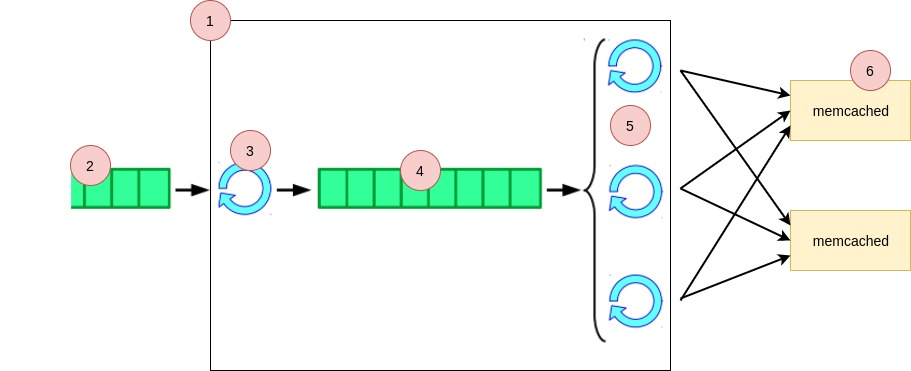
\includegraphics[width=0.8\textwidth ]{images/mw_architecture.jpg}
    \caption{Simplified System Architecture including the Middleware (1), Network Queue (2), Main Thread (3), Middleware Queue (4), Worker Pool (5) and the Memcached Servers (6).}
    \label{fig:system_arch}
\end{figure} 


At the other end of the queue a worker thread, being part of the worker pool (all nr. 5), dequeues the request. The worker threads are instances of the Worker.java\footnote{\url{https://gitlab.ethz.ch/siegli/asl-fall17-project/blob/master/src/ch/ethz/asltest/siegli/workers/Worker.java}} class and a subclass of the java.lang.Thread\footnote{\url{https://docs.oracle.com/javase/8/docs/api/java/lang/Thread.html}} class. They maintain a TCP connection (java.nio.channels.SocketChannel) to each memcached server (6). Depending on the request type (GET, MULTIGET, SET) and the operation mode (sharded/non-sharded) they forward the request to the corresponding server(s). The load balancing is taken care of by the main thread and will be explained in subsection \ref{sub:load_balancing} . Before fetching a new request from the middleware queue (4) again the worker thread waits for the response(s) of the server(s), parses them and send them back to the clients. The blocking behaviour of the middleware queue makes sure that a thread frees it's resources for other workers if there is no pending request in the queue. Also during the time a worker has to wait for the response of a memcached server it allows for being rescheduled as the SocketChannel is set to be blocking. 
\subsection{Timestamps}\label{sub:timestamps}

In order to measure the middleware the following timestamps will be used throughout the rest of the project. As mentioned before, each MemcachedTask class has a corresponding attribute. The number correspond to those of Figure \ref{fig:timestamps}.

\begin{enumerate}
\item $T_{startMiddleware}$  Timestamp of having created the MemcachedTask object.
\item $T_{startQueue}$  Timestamp after having enqueued the MemcachedTask object
\item $T_{stopQueue}$   Timestamp after having dequeued the MemcachedTask object
\item $T_{startServer}$  Timestamp after having forwarded the request to the server
\item $T_{stopServer}$  Timestamp after having received the response from the server. In the case of sharded MULTIGETS and WRITEs to multiple servers this means after having received all responses and also having parsed them.
\item $T_{stopMiddleware}$ Timestamp after having sent the response back to the client


\end{enumerate}

It holds that $T_{startMiddleware}$ $<$ $T_{startQueue}$ $<$ $T_{stopQueue}$ $<$ $T_{startServer}$ $<$ $T_{stopServer}$  \\$<$ $T_{stopMiddleware}$ where '$<$' is to be read as 'happened before in time'.\\

\begin{figure}
    \centering
    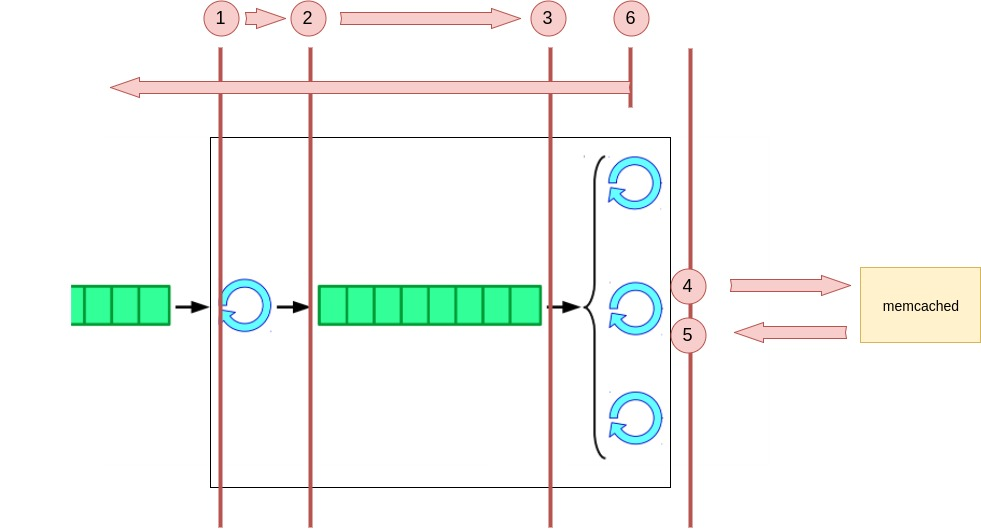
\includegraphics[width=0.8\textwidth ]{images/mw_timing.jpg}
    \caption{Timestamps used during the project}
    \label{fig:timestamps}
\end{figure}

From above timestamps we deduce the following definition. Whenever talking about middleware measurements we refer to these definitions.

\begin{itemize}
    \item Middleware Time \tb{(MWT)} or Response Time  =  $T_{stopMiddleware}$ - $T_{startMiddleware}$
    \item Queue Waiting Time \tb{(QWT)} =  $T_{stopQueue}$ - $T_{startQueue}$
    \item Service Time \tb{(ST)} =  $T_{stopServer}$ - $T_{startServer}$
\end{itemize}


\subsection{Request Parsing and Buffers}\label{sub:req_parsing_buffers}
As mentioned the messages are parsed by the main thread before being pushed to middleware queue. This implies that the parsing time should be kept as minimal as possible since it would prevent the main thread from accepting other network packets leading to an increasing network queue. Therefore, the RequestParser.java\footnote{\url{https://gitlab.ethz.ch/siegli/asl-fall17-project/blob/master/src/ch/ethz/asltest/siegli/protocol/RequestParser.java}} class avoids calls such as copying buffers and creating new Strings which would lead to an increased processing time and memory usage. The RequestParser rather directly operates on the java.nio.ByteBuffer into which the message was read initially and tries to reuse them in the following way.

\subsubsection*{Buffer Reuse}
Each RequestParser maintains an allocated ByteBuffer of 2 kBytes which is enough for a MULTIGET request with 10 keys and a WRITE request with 1kByte data. Upon accepting a new connection from a client, the middleware creates a new RequestParser object and stores the association to the client connection in a map. Like this we only allocate roughly 3 kBytes of memory per client once when a we accept a new connection. Whenever a new request from a client arrives the middleware will fetch the corresponding RequestParser which will then process it. After having parsed the message, the RequestParser stores the reference to it's Buffer in the newly created MemcachedTask object. This will later on be used by the worker thread which upon forwarding the request to the server will simply flip the buffer (i.e. make it readable) and write it's content into the SocketChannel(s) of the corresponding servers. An exception to this is the sharded-MULTIGET case where we split the original requests into smaller requests and write them into an additional buffer but also this one will be reused.\\

In order to process the answers from the servers, each Worker makes use of the functionality of it's ResponseParser.java\footnote{\url{https://gitlab.ethz.ch/siegli/asl-fall17-project/blob/master/src/ch/ethz/asltest/siegli/protocol/ResponseParser.java}} object. The ResponseParsers have three fixed allocated ByteBuffers dedicated to the three different request types (GET, MULTIGET, SET). While the response buffer for GET requests is fixed to 1.5 kBytes the MULTIGET buffer has a size of 15 kBytes. This is due to the fact that we use data values of 1 kByte size and therefore the chosen sizes are enough for a single GET and a MULTIGET having maximal 10 keys. The buffer for the SET response is only 512 Bytes large since we either expect an \ti{ERROR} or \ti{STORED} as a response. After finishing parsing the response the Worker forwards it by writing the bytes from the buffer into the SocketChannel of the client as pointed out in subsection \ref{sub:architecture}. The response parsing process will be explained a bit more in detail in subsection \ref{sub:resp_parsing}.\\

The above described implementation allows us to allocate the required buffer memory only once leading to a more stable memory usage pattern since frequent memory allocation and deallocation requests are avoided. 

\subsubsection*{Request Parsing}
In order to parse an incoming message a RequestParser proceeds as follows:

\begin{enumerate}
    \item Read the received bytes from the network queue into the request buffer.
    \item If a memcached commandline is complete (according to the protocol specifications \cite{memcached_protocol}) which means a \ti{return character} was received  proceed else go to 1.
    \item Define the message type by looking at the first three bytes (GET or SET) and counting the number of keys. If a get request has more than one key it gets parsed into a MULTIGET MemcachedTask.
    \item In the case of a GET or MULTIGET create a new MemcachedTask and return it.
    \item In the case of a SET parse the last number of the command telling the number of bytes of the data.
    \item If all data has been read, create a new MemcachedTask and return it. Otherwise go back to 1.
    
\end{enumerate}

Note that the above procedure also allows the requests being split over multiple network packets which is likely to happen in case of large SET requests. 



\subsection{Load Balancing}\label{sub:load_balancing}
If the middleware is connected to more than one memcached server, the requests have to be distributed evenly amongst them. For WRITE requests this means that they are replicated to all servers. For GET  and MULTIGET in non-sharded mode, the main thread assigns each MemcachedTask the id of the server (in a round robin manner) to which the request should be sent to by the worker threads. To convince ourselves that this achieves a fair sharing, the middleware was instrumented to count the number of requests sent to each server. First the three memcached servers were populated with a write-only and afterwards with a read-only payload. The result for the read-only payload with three memcached servers is shown in Figure \ref{fig:load_bal_mw}. One can see that in each aggregation window the servers received a fair share (33\%) of the total number of GET requests. Figure \ref{fig:load_bal_server} shows the output of sending a memcached \tt{stats} to each server after having run the above experiment. One can see that the WRITE requests are replicated to all servers (cmd\_set) and that each server received the same total amount of GET requests (cmd\_get). In case the middleware is set to sharding-mode the keys are distributed evenly to all servers and if the number of keys is not divisible by the number of servers the rest of the division is split to the servers starting with the first one. For example with 5 keys and 3 servers, server1 and server2 would get 2 keys and server3 one key.


\begin{figure}
    \centering
    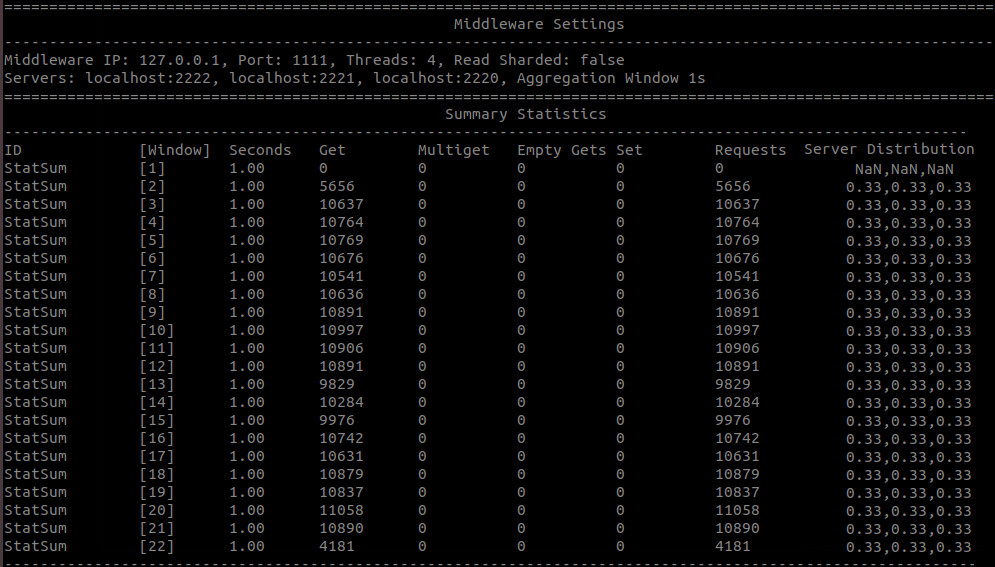
\includegraphics[width=0.8\textwidth ]{images/load_bal_mw_stat.jpg}
    \caption{Middleware output showing that the GET requests are distributed evenly (33\%) among the three memcached server.}
    \label{fig:load_bal_mw}
\end{figure}

\begin{figure}
    \centering
    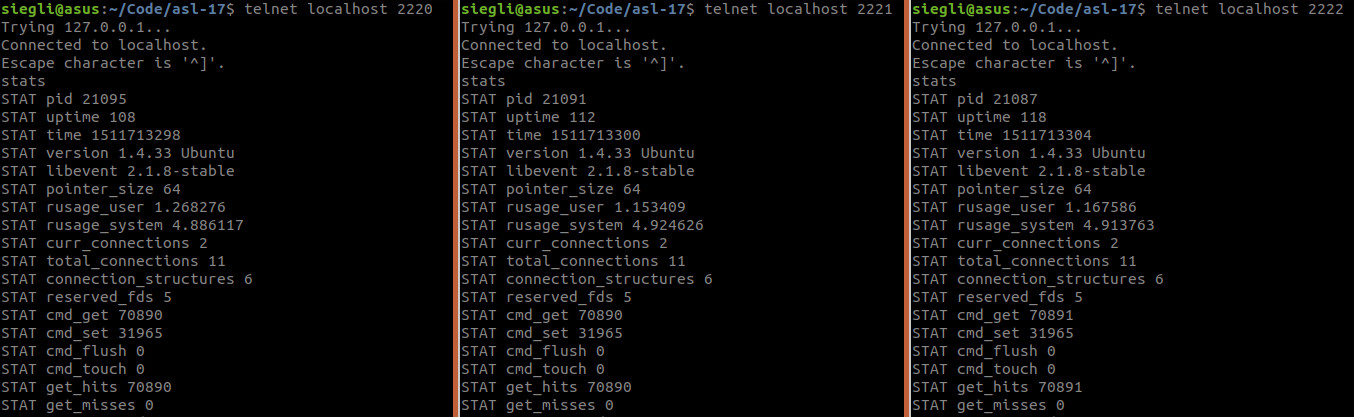
\includegraphics[width=\textwidth ]{images/load_bal_server_stat.jpg}
    \caption{Memcached output of sending a \tt{stats} to each server after sending a write-only payload followed by a read-only payload. One can see that the WRITE requests are replicated to all servers (cmd\_set) and that each server received the same total amount of GET requests (cmd\_get).}
    \label{fig:load_bal_server}
\end{figure}


\subsection{Response Parsing}\label{sub:resp_parsing}
After having sent the request to the server each Worker waits (blocking) for the response which will be read into a different buffer depending on the type of the request (see subsection \ref{sub:req_parsing_buffers}). If multiple servers are involved we first send the requests to all servers before starting with parsing the responses. The handling of the responses will now be explained a bit more in detail for all three request types individually. The described functionality is all implemented by the ResponseParser.java\footnote{\url{https://gitlab.ethz.ch/siegli/asl-fall17-project/blob/master/src/ch/ethz/asltest/siegli/protocol/ResponseParser.java}} class.


\subsubsection*{SET Requests}
For SET requests we either expect a \ti{STORED} or an \ti{ERROR} response from the memcached server. In the case of multiple servers we wait until having received all responses and then either forward \ti{STORED} if no error occurred or otherwise the last received error message back to the client.

\subsection*{GET Requests}
For (single) GET requests we proceed as follows:
\begin{enumerate}
    \item Read the received bytes into the buffer.
    \item \begin{itemize}
        \item If the response starts with \ti{VALUE} we increase the "nofPackets-counter" by one and parse the last digit of the current line which will tell the size of the response and therefore the buffer index of the next expected command line. If enough bytes have been read check if we received an \ti{END} at the expected place in the buffer otherwise go back to 1 and proceed until the response is complete (i.e. we received \ti{END}).
        \item If the response starts with \ti{END} this means the value could not be found in the cache.  
        \item If we receive \ti{ERROR} there was an error and we are also done.
    \end{itemize}
    \item Return the response to the client by writing the buffer bytes into the client's SocketChannel stored in the MemcachedTask.
\end{enumerate}

\subsubsection*{MULTIGET Requests}
In the \tb{non-sharded} case we proceed exactly as in the (single) GET case above. As we keep track of the number of received messages (i.e. number of \ti{VALUE} command lines) we know at the number of cache-misses and can set it in the MemcachedTask.
In the \tb{sharded} case the response parsing stays the same except that we parse the responses from the different servers in the order we sent the requests but still with the same procedure. A bit more care has to be taken in the case of receiving an error. If there is one or more errors from a server we return the last one received to the client.\\

The central function for parsing all different GET requests can be found in the ResponseParser class and is mainly implemented by \tt{readCheckAndCountGetResponses()}. Note that as with parsing the requests we also operate directly on the buffers here. This avoids unnecessary data copies and therefore processing time and memory consumption. Furthermore do above procedures ensure that we correctly parse responses split over multiple network packets which is very likely for MULTIGET responses which can be of size more than 10 kBytes. 

\subsection{Call Chain}\label{sub:reqProcessing}
To summarize the request processing, Listing \ref{lst:req_processing} shows a chronological sequence of the most important function calls involved in processing a SET request. For the other request types one can simply replace the functions with the corresponding request type names (e.g processGet -$>$ processSingleGet). An indentation means that the call is part of the previous method and upper case notation does not mean that a static procedure call is made but rather the function is implemented by that class.


\lstset{language=Java, caption={Most important function calls and components involved in processing a SET request.}, label={lst:req_processing}}
\begin{lstlisting}[frame=single]
MemcachedTask task = RequestParser.parseMessage(clientSocketChannel);
MyMiddleware.enqueue(task);
MemcachedTask task = Worker.dequeue();
Worker.processSet(task);
   Worker.sendMsgToServer(task);
   ResponseParser.parseSetResponse(task, serverSocketChannels);
   Worker.sendResponseBackToClient(task, ResponseParser.setBuffer);
\end{lstlisting}


\subsection{Collecting Statistics}\label{sub:stat}
In order to evaluate the middleware performance, each MemcachedTask object contains the timestamps as described in subsection \ref{sub:architecture} together with numbers such as queue length, number of requests and so on. In order to gather these statistics each worker maintains a list of Statistics.java\footnote{\url{https://gitlab.ethz.ch/siegli/asl-fall17-project/blob/master/src/ch/ethz/asltest/siegli/workers/Statistics.java}} objects (history). Each Statistics object contains the aggregated values collected within one aggregation window. The values are updated by the Worker by calling \tt{updateStatisitcs(MemcachedTask)} on it's current Statistics object after having processed a request. The averages are directly calculated online.
The StatisticsUpdaterTask.java\footnote{\url{https://gitlab.ethz.ch/siegli/asl-fall17-project/blob/master/src/ch/ethz/asltest/siegli/workers/StatisticUpdaterTask.java}} which is a subclass of the java.util.TimerTask\footnote{\url{https://docs.oracle.com/javase/8/docs/api/java/util/TimerTask.html}}
 periodically (every aggregation windows size) loops over all Workers and on each of them calls \tt{setNewStatisticsWindow()}. This method adds the Worker's current Statistics object to the history and creates a new current Statistics object. This method ensures that all the worker threads update their Statistics object "simultaneously" which is important if we summarize the values at the end. Having a look at the \ti{Seconds} column of the middleware output in Figure \ref{fig:load_bal_mw} gives us the confirmation that indeed these windows are always of the same size. By looking at the used memory size during an experiment run of 2 minutes we chose to set the aggregation window size to 1 second since no performance limiting increase could be observed.
 \\In order to summarize the values collected by each individual thread the Finalizer.java\footnote{\url{https://gitlab.ethz.ch/siegli/asl-fall17-project/blob/master/src/ch/ethz/asltest/siegli/workers/Finalizer.java}} class merges the different result when the middleware is shutdown by an interrupt. This is achieved by adding a shutdown hook\footnote{ https://docs.oracle.com/javase/8/docs/api/java/lang/Runtime.html\#addShutdownHook(java.lang.Thread)} to the java Runtime at middleware startup time. The Finalizer thread also prints the merged results to a log file.\\
 In addition to the so far mentioned measurements each Worker keeps track of the middleware response times over the whole middleware lifetime in the form of a histogram. It does so by allocating a fixed size array at start up where the index represents a 100 $\mu$s histogram slot and the corresponding value the number of measured response times in this slot. The last array entry contains the number of response times which were possibly larger than $100\mu s * number\_of\_array\_slots$. Choosing the array size is a trade off between memory usage and precision. It should therefore be set after having run the experiment for a short time giving some insights on the to be expected response times.

 
\subsection{Logging}
After starting the middleware the \ti{/logs} directory contains three files. While \ti{timing.log} contains all the data regarding the middleware measurements, \ti{info.log} and \ti{error.log} contain log entries used for information/debugging and error handling, respectively. The chosen logging strategy (as described in \ref{sub:stat}) has the big advantage that we do not use CPU cycles for i/o requests during runtime as we only log when the middleware is shut down.




\section{Baseline without Middleware (75 pts)}\label{sec:bl_without_mw}

To get a feeling for the performance of the memcached servers and the memtier clients we will run some baseline experiments. During all experiments we also logged other system relevant metrics using \tt{dstat}\footnote{\url{http://dag.wiee.rs/home-made/dstat/}} on every machine. In order to have a ground truth for the latency between two machines we used \tt{ping}.
Each experiment was conducted over 60 seconds. From the output of memtier, which are one second aggregated statistics measurements, we first eliminated the startup and cooldown phase (2 seconds each) and then took the average over the remaining windows. Afterwards we averaged the measured response times and summed up the number of transactions per second of all memtier instances. Finally, for summarizing the different runs we again take the average of the measurements and the average of the variances of the individual repetitions.
Before starting with the experiments we populate the memcached servers with a write-only payload in order that all possible keys mermtier-\{1-10000\} are present. This is done to avoid the impact of "empty-gets".

\subsection{One Server}

In a first experiment we used one memcached server and three load generating client machines to find out the behavior of the server depending on the number of clients.
The exact parameters can be found in the below table. From now on we will use the abbreviations w-o and r-o for write-only and read-only, respectively.

\begin{center}
	\scriptsize{
		\begin{tabular}{|l|c|}
			\hline Number of servers                & 1                        \\ 
			\hline Number of client machines        & 3                        \\ 
			\hline Instances of memtier per machine & 1                        \\ 
			\hline Threads per memtier instance     & 2                        \\
			\hline Virtual clients per thread       & [1 4 8 12 16 20 24 28 32]                  \\ 
			\hline Workload                         & Write-only and Read-only \\
			\hline Multi-Get behavior               & N/A                      \\
			\hline Multi-Get size                   & N/A                      \\
			\hline Number of middlewares            & N/A                      \\
			\hline Worker threads per middleware    & N/A                      \\
			\hline Repetitions                      & 3              \\ 
			\hline Duration [sec]                   & 60              \\ 
			\hline 
		\end{tabular}
	} 
\end{center}


\begin{figure}
\centering
\begin{subfigure}{.5\textwidth}
    \centering
    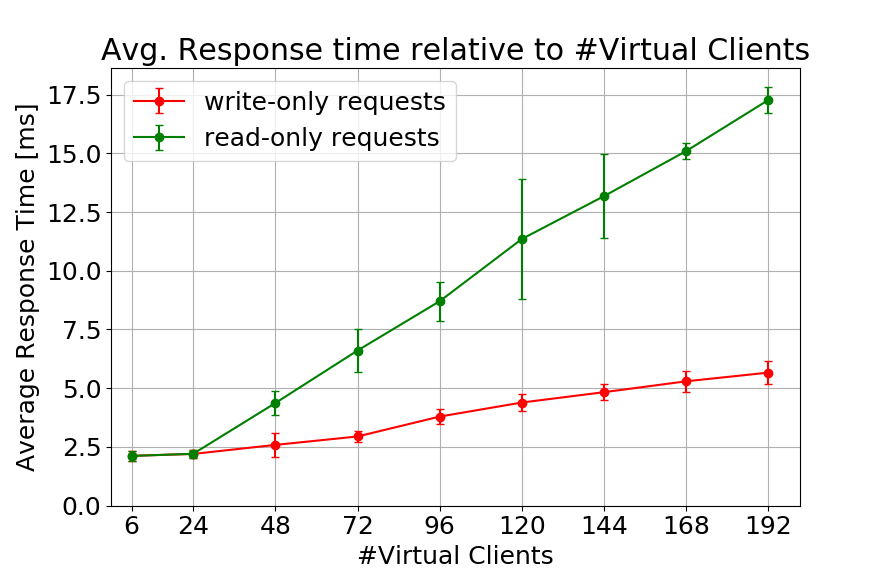
\includegraphics[width=0.8\textwidth ]{plots/baselineWithoutMw/rt_one_server_1.png}
    \caption{Average Response Time }
    \label{plt:bl:rt_one_server_1}
\end{subfigure}%
\begin{subfigure}{.5\textwidth}
    \centering
    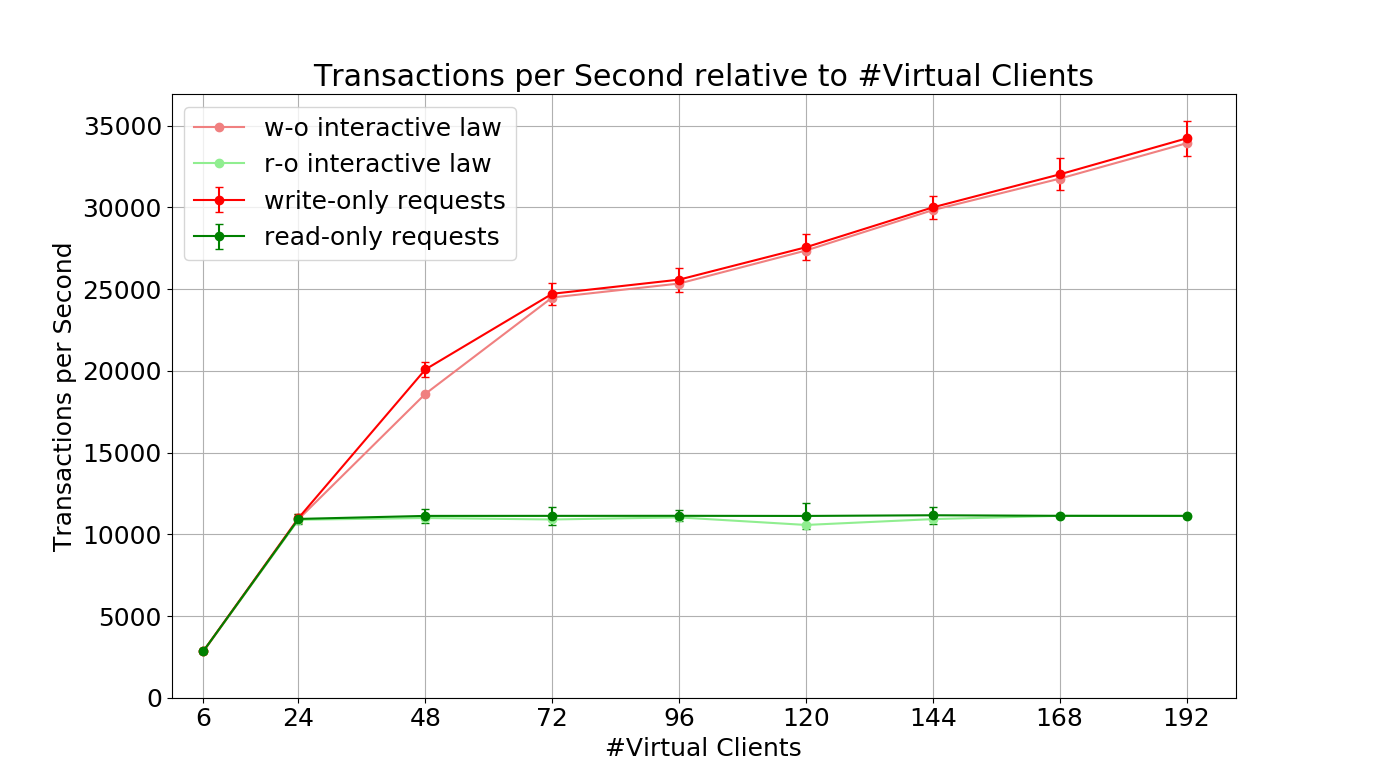
\includegraphics[width=\textwidth ]{plots/baselineWithoutMw/tp_one_server_1.png}
    \caption{Average Throughput and Interactive Law}
    \label{plt:bl:tp_one_server_1}

\end{subfigure}
\caption{Results for a write-only and read-only payload measured for one memcached server and different number of virtual clients. The errorbars show the standard deviations of the corresponding averages over 3 runs.}
\label{plt:bl:one_server_1}
\end{figure}





\subsubsection{Explanation}

The result of the experiment is shown in Figure \ref{plt:bl:one_server_1}. In the following we will discuss the main observation based on that figure.
When reasoning with available bandwidth we refer to the results of the bandwidth experiment in subsection \ref{sub:bw_measurements}.

\paragraph{Difference between w-o and r-o payload}
The first noticeable observation is the big difference between the w-o payloads (red) and the r-o payloads (green). When looking at the number of transactions per second (Figure \ref{plt:bl:tp_one_server_1}) we can see that there seems to be a hard limiting factor for the r-o payloads. When looking closer the throughput stops increasing for 11'000 read requests per second. As the data has a size of 1kB (get request payload) and we have some overhead for each request (packet header, request command line) this corresponds very closely to the calculated maximum outgoing (upstream) network bandwidth of 12.5 MB/s for the memcached server in subsection \ref{sub:bw_measurements}. As the incoming (downstream) bandwidth is much higher ($>$ 600 Mb/s) the set requests (w-o payload) are not affected by this limiting factor. By looking at the data used to generate the plots\footnote{\url{https://gitlab.ethz.ch/siegli/asl-fall17-project/tree/master/experiment_outputs/useful/baseline_without_mw/baseline_one_server_1/plot_data}} we see that the more precice maximal throughput is 11121 requests per second (rps). Together with the maximum available bandwidth of 12.5 MB we conclude that one request has an approximate size of $\frac{12.5 MBps}{11121rps} = 1.12 MBpr$ (pr=per request).
As the throughput is upper bounded and we increase the number of clients this means that due to the interactive law the response times should grow linearly as illustrated in Figure \ref{plt:bl:rt_one_server_1}. While the get requests are limited by bandwidth the set requests (w-o payloads) are not because they only involve request payloads being sent from the memtier clients to the memcached server. The throughput increases up 34'000 for 192 clients. However, there is a knee at 72 clients after which the slope starts decreasing. The reason for this might be the increasing number of connections/requests that the memcached server has to handle. This increases the overhead for context switching and synchronization which means the performance gain decreases. This can also very nicely be seen in the \tt{dstat} output file of the server\footnote{\url{https://gitlab.ethz.ch/siegli/asl-fall17-project/blob/master/experiment_outputs/useful/baseline_without_mw/baseline_one_server_1/dstat_server1.txt}}. When looking at the CPU idle time (showing how busy the machine is) we can see that for the w-o payloads it starts with 95\% for 6 clients and decreases down to 40\% for 192 clients clearly indicating that the server has more work to do. For the r-o payload there is no difference in CPU idle time between 6 and 192 clients as the bandwidth is limiting the speed of the server's responses and therefore the server does not get enough requests to get saturated. 


\paragraph{Correlation of throughput and response time}
The relation between the response time and the throughput is $TP = 1000 \times \frac{\#clients}{RT}$ according to the interactive law. We have to multiply with 1000 because of the time being measured in milliseconds and assume a (memtier-) client thinking time of zero. Based on the measured response times we calculated the to be expected throughput according to that formula and plotted the result together with the measured throughput in Figure \ref{plt:bl:tp_one_server_1}. The two lines nearly cover except from the w-o point for 48 clients and r-o point for 120 clients. The reason for this might be that for these points we had some bigger deviation of the measured response times between the different memtier instances as can be seen in Figure \ref{plt:bl:rt_one_server_1}.

\paragraph{Standard Deviations}
Looking at the response time plot we see some larger response time standard deviation for w-o, 48 clients. By inspecting the log files\footnote{\url{https://gitlab.ethz.ch/siegli/asl-fall17-project/blob/master/experiment_outputs/useful/baseline_without_mw/baseline_one_server_1.zip}} one can see that there was a higher response time in run 2. This can happen since we measure in the cloud and not in a closed environment and therefore have to deal with influences out of our control. This could for example mean that another VM running next to ours consumed more resources. For the r-o curve we have a large response time standard deviation for 120 and 144 clients. There looking at different runs was not enough and we had to differentiate between the different machines. Interestingly client3 received much faster responses than client2 for 120 and 144 clients over all three runs (more than the difference in network latency). Therefore, it can not be explained with temporal increase in load as before. A reason might be that due to the limiting bandwidth the network share was not allocated fairly between the three machines or the time of 60 seconds was at least not enough to converge to a fair distribution according to the TCP congestion control algorithm. 

\paragraph{Saturation}
While the system is naturally saturated with 24 clients for the r-o payloads (due to the bandwidth) there is no clear saturation point noticeable for the set request payload. Out of this we conducted another experiment with the numbers of clients ranging from 1 up to 64 per memtier thread (6 to 384 virtual clients in total). The result is shown in Figure \ref{plt:bl:one_server_2}. By looking at the throughput plot one can say that for the w-o payloads the system is saturated for 192 clients. There even seems to be an over-saturated phase (336) clients. By having a look at the \tt{dstat} file of the server\footnote{\url{https://gitlab.ethz.ch/siegli/asl-fall17-project/blob/master/experiment_outputs/useful/baseline_without_mw/baseline_one_server_2/dstat_server1.txt}} one can see that the the CPU idle times shrink down to 0\% after crossing the 192 clients mark indicating that the server is fully saturated. Besides these observations there is another big difference to the previous experiment namely the response time for clients in the range of 6 to 72. For 6 clients the average response time jumped from previously 2.1 ms to 0.5 seconds. This can only be explained by the fact that between the two experiments the machines were stopped and new started which means they can also be reallocated to different physical machines. A delay of 0.5 milliseconds is probably the case if all virtual machines are on the same physical machine. This small delay has a big impact on the throughput. In the case where previously 6 machines were not yet enough to produce enough traffic this is now possible and for the r-o payloads we already have a saturated system with 6 clients. With an increasing number of clients the impact of the network delay starts decreasing since the delay imposed by the memcached server starts taking overhand. Therefore after 72 clients the two experiments are again comparable.


\begin{figure}[H]
\centering
\begin{subfigure}{.5\textwidth}
    \centering
    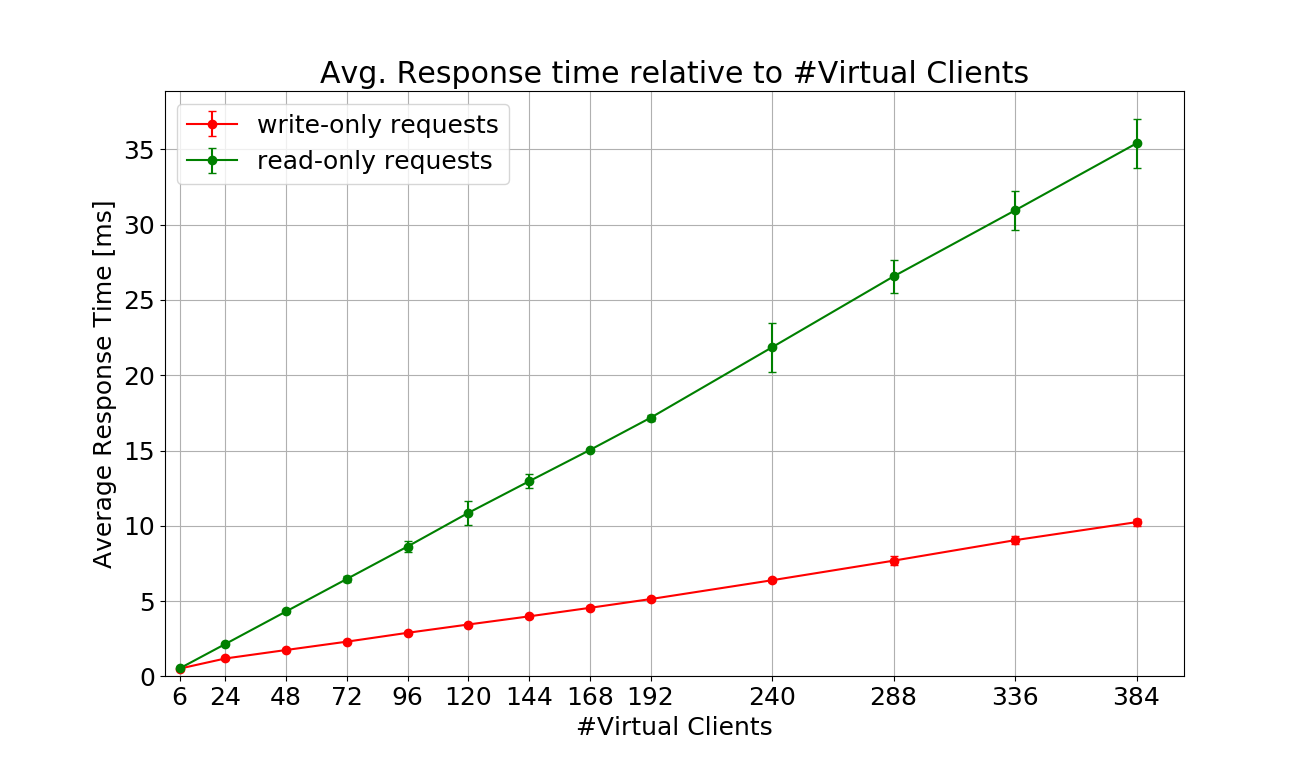
\includegraphics[width=\textwidth ]{plots/baselineWithoutMw/rt_one_server_2.png}
    \caption{Average Response Time }
    \label{plt:bl:rt_one_server_2}
\end{subfigure}%
\begin{subfigure}{.5\textwidth}
    \centering
    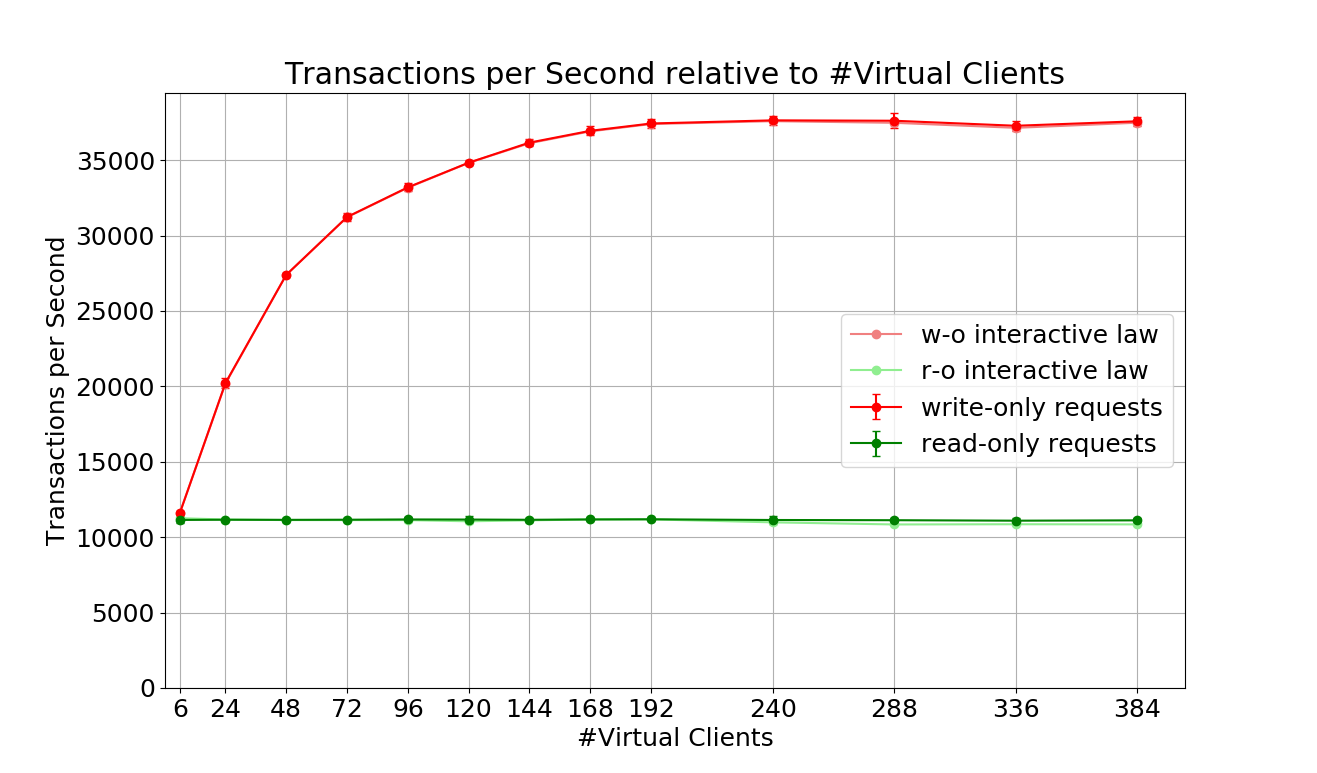
\includegraphics[width=\textwidth ]{plots/baselineWithoutMw/tp_one_server_2.png}
    \caption{Average Throughput and Interactive Law}
    \label{plt:bl:tp_one_server_2}

\end{subfigure}
\caption{Results for a write-only and read-only payload measured for one memcached server and different number of virtual clients. The errorbars show the standard deviations of the corresponding averages. The number of clients was increased to up to 64 per memtier thread.}
\label{plt:bl:one_server_2}
\end{figure}





\subsection{Two Servers}

In a second experiment we wanted to analyze the behavior of a memtier client by adding a second memcached server and only using one load generating machine. Th client machine runs two memtier instances where each instance is connected to one server. Since last time we were not sure whether we hit the sweet spot with 32 clients we directly used an extended range for the number of virtual clients per thread. The exact experiment parameters are again listed in the table below.


\begin{center}
	\scriptsize{
		\begin{tabular}{|l|c|}
			\hline Number of servers                & 2                        \\ 
			\hline Number of client machines        & 1                        \\ 
			\hline Instances of memtier per machine & 2                        \\ 
			\hline Threads per memtier instance     & 1                        \\
			\hline Virtual clients per thread       & [1 4 8 12 16 20 24 28 32 40 48 56 64]                  \\ 
			\hline Workload                         & Write-only and Read-only \\
			\hline Multi-Get behavior               & N/A                      \\
			\hline Multi-Get size                   & N/A                      \\
			\hline Number of middlewares            & N/A                      \\
			\hline Worker threads per middleware    & N/A                      \\
			\hline Repetitions                      & 3                 \\ 
			\hline Duration [sec]                      & 60              \\ 
			\hline 
		\end{tabular}
	} 
\end{center}

\subsubsection{Explanation}
Figure \ref{plt:bl:one_client} shows the results of the above experiment. We ommitted the results for 104 and 128 clients since there was no significant difference to 96 clients. We also left one data point out, namely the r-o, 12 clients(per thread) in run 1 for instance 1. The reason was a response time of over 500 milliseconds in one of the aggregation windows, leading to a big deviation. Since the other runs and the other instance looked very different we claim that it has nothing to do with our experiment and can therefore be treated as an outlier. We see that compared to before the two different payloads look very similar this time. This migth come from the fact that we have an available bandwidth of 200 Mb/s for both since we have one memtier machine and two memcached client. Moreover, at first sight it does not look like the bandwidth is the limiting factor since there is no sharp cut but this will be analyzed in more detail soon. Now that we can compare the two payloads we can say that there is no difference between a set and a get request for this setup in terms of processing time. Or at least the difference in how the load generator and the memcached server handle the two different request types is not noticeable as the processing time difference is likely to be overwhelmed by the delay imposed by the network. From the plot we can see that the system reaches a saturation state for 56 clients as from there on the response time only starts increasing but the throughput does not change significantly.

 In order to reason more precisely about the saturation of w-o payload the let's have a look at the throughput data used to generate the plots which can be found here\footnote{\url{https://gitlab.ethz.ch/siegli/asl-fall17-project/tree/master/experiment_outputs/useful/baseline_without_mw/baseline_one_client/plot_data}} We only show the numbers up to 56 clients and the values for the w-o payloads since afterwards the system is saturated.
\verbatimfont{\small}%
\begin{verbatim}
Throughput [1k requests/sec] for a w-o payload and for two 
memcached servers and one memtier client machine.

       2         8         16        24        32         40         48         56    
     989      3844       7515     10857     13912      16538      19995      21716    


\end{verbatim}

From the previous subsection we know that one request has an approximate size of 1.12 MB. So our maximal throughput (see table) of 21716 rps corresponds to a throughput of \ti{1.12 MB/request $\times$  21716 requests/second $\approx$ 24.3 MB/s}. As we have measured in subsection \ref{sub:bw_measurements} the outgoing bandwidth for a memtier machine is 25 MB/s. This means that we probably reached the maximum outgoing bandwidth limit of a memtier client machine and that neither the memtier client nor the memcached server came to their limits. This can also be seen in the \tt{dstat}\footnote{\url{https://gitlab.ethz.ch/siegli/asl-fall17-project/tree/master/experiment_outputs/useful/baseline_without_mw/baseline_one_client}} files of the machines which again show the outgoing bandwidth limits for the client (~24 MB/s) and for the servers (~12 MB/s). Furthermore by looking at the CPU idle times we see that neither the memtier machine (77\%) nor the servers (92\%) are a limiting factor for 32 clients. Compared to last time the client is however, more busy since we have only one load generating machine for two servers. Note that while for the w-o payloads the bandwidth of the client (200 Mb/s) is the limiting factor for the r-o payload the bandwidth of the servers (2$\times$100 Mb/s) is the barrier. As a short summary we have seen that one memtier machine is able to generate enough set and get requests to saturate it's own outgoing bandwidth as well as the one of two memcached servers, respectively.

\begin{figure}
\centering
\begin{subfigure}{.5\textwidth}
    \centering
    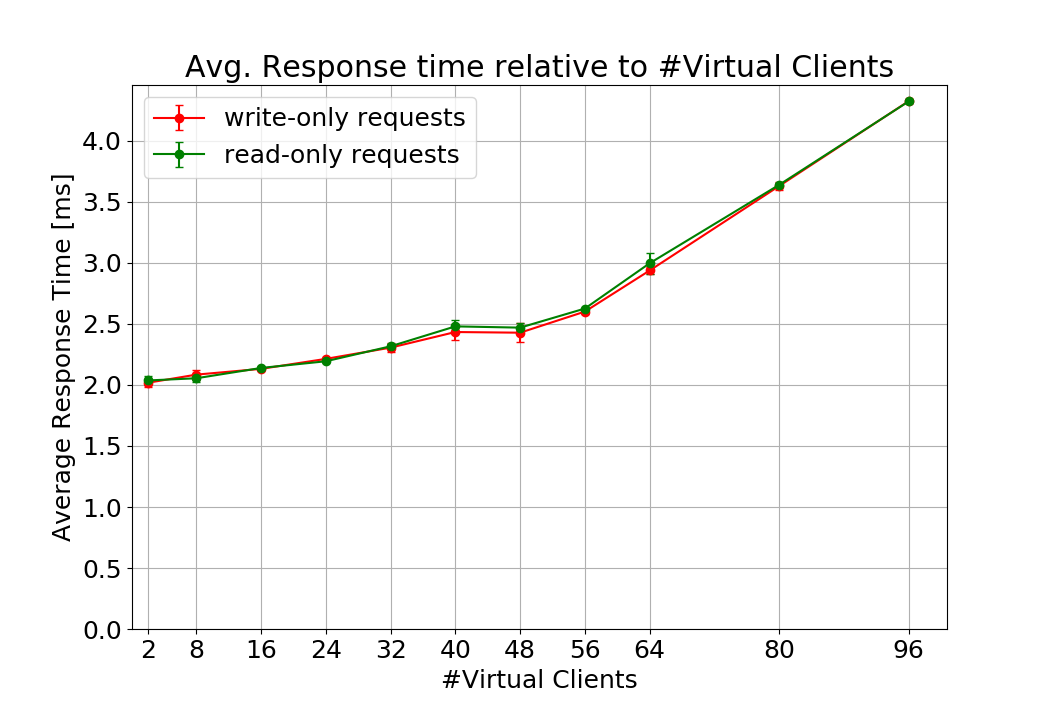
\includegraphics[width=\textwidth ]{plots/baselineWithoutMw/rt_one_client.png}
    \caption{Average Response Time }
    \label{plt:bl:rt_one_client}
\end{subfigure}%
\begin{subfigure}{.5\textwidth}
    \centering
    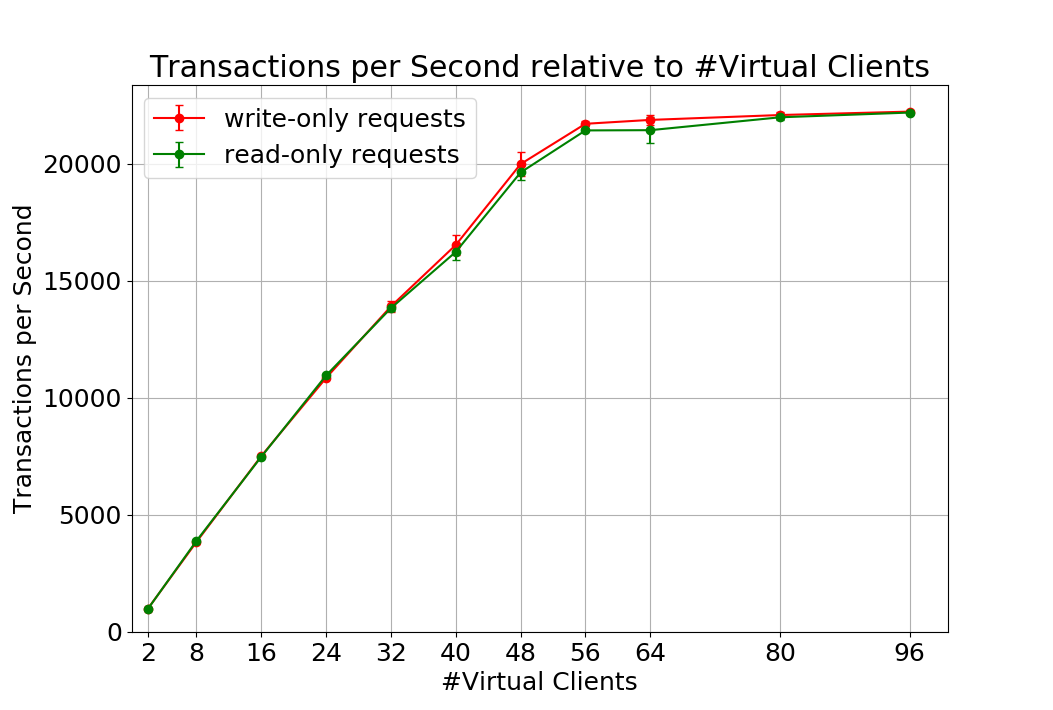
\includegraphics[width=\textwidth ]{plots/baselineWithoutMw/tp_one_client.png}
    \caption{Average Throughput}
    \label{plt:bl:tp_one_client}

\end{subfigure}
\caption{Results for a write-only and read-only payload measured for TWO memcached servers and ONE memtier client machine with different number of virtual clients. The errorbars show the standard deviations of the corresponding averages.}
\label{plt:bl:one_client}
\end{figure}




\subsection{Summary}\label{sub:bl_without_summary}

\begin{center}
	{Maximum throughput of different VMs.}
	\begin{tabular}{|l|p{2cm}|p{2cm}|p{4cm}|}
		\hline                        & Read-only workload & Write-only workload & Configuration gives max. throughput \\ 
		\hline One memcached server   &        11155         &         37426            &      6/24 clients depending on  network delay and 192 clients for w-o                         \\ 
		\hline One load generating VM &        21433            &         21716     &              56 clients                       \\ 
		\hline 
	\end{tabular}
\end{center}

From the first experiment we know that for a read-only payload a memcached server (or better it's VM) is bound to roughly 11k requests per second due to it's outgoing bandwidth limit of 12.5 MB/s. This means that with 3 memcached VM's we can never expect to see a r-o payload that exceeds 37.5 MB/s or roughly 33k rps. This can for example very well be seen by comparing the first with the second experiment. There we see that for the r-o payload the throughput roughly doubles as we double the number of memcached machines. The limitations for the w-o payloads either (depending on the setup) come from the outgoing bandwidth of the memtier machines or from the memcached server's resource limitations. First could be observed in the experiment with two servers. There we measured a maximum throughput of 25 MB/s or roughly 22k rps for one memtier machine. This means we should never expect to see a w-o throughput of more than 75 MB/s or 66k rps for 3 client machines. The throughput bottleneck arising from the memcached server's resource limitations was observed in the first experiment where we saw that for roughly 37k rps the server starts getting overloaded. This means when only using one server this is an upper limit. However, adding a second server would already be enough because we can only use 3 memtier machines which could not produce enough requests since $3\times22k < 2\times37k$. We also conclude that using 64 clients per memtier machine are sufficient to produce enough load to saturate the bottlenecks  but this also depends on the delay of the network between the different machines.\\
Above findings are summarized in the table below. For the memtier machines we do not know the exact limitations of a r-o workload since we probably would not have enough memcached machines. We certainly know that it can generate more than 22k rps from the last experiment and since the machine was pretty idle deduce that it should also be enough for 3 memcached servers (i.e 33k rps) \\

\begin{table}
    \centering
    \begin{tabular}{|p{4cm}|p{2cm}|p{2cm}||p{6cm}|}
		\hline                        & Write-only workload & Read-only workload  & Reasons (BW = bandwidth)  \\ 
		\hline 1 memtier machine can generate   &        22k       &            $>$ 33k & memtier BW / memcached BW        \\ 
		\hline 1 memcached machine can handle &        37k            &         11k        & memcached system resources (CPU,RAM,..) / memcached BW     \\ 
		\hline 
	\end{tabular}
    \caption{Maximum throughput in transactions per second that we can expect from a corresponding machine.}

\end{table}
	


\subsection{Bandwidth Measurements}\label{sub:bw_measurements}
Since it seems to be a crucial parameter we analyzed the available bandwidth between the memtier client (Basic A2 : 2 vcpus, 3.5 GB memory) and the memcached server (Basic A1 : 1 vcpu, 1.75 GB memory) machines. For this we used the freely available tool \tt{iperf}\footnote{\url{https://iperf.fr/}}. \\
First we ran the iperf server on the server machine (\tt{iperf -s}) and connected to it from one client machine (\tt{iperf -c IPserver1 -t 30}) for 30 seconds. From the result shown in Figure \ref{fig:bl:iperf_cl_server} we can conclude that the outgoing bandwidth of a memtier machine is bound to 200 Mb/s or 25 MB/s.
In a next step we connected one iperf client on every memtier machine to the iperf server on the memcached machine. The result looked very similar to the previous one except that the received bandwith on the server was 600 Mb/s showing that the inbound bandwith of the memcached server is at least 600 Mb/s.
In a last step we tested the outgoing bandwith of the memcached machine. For this we flipped the setup of the first experiment such that the iperf server was running on the memtier machine and the iperf client on the memcached machine. The result in Figure \ref{fig:bl:iperf_server_cl} shows that the outgoing bandwith for a memcached machine is limited to 100 Mb/s or 12.5 MB/s. The summary of available bandwidths is listed in Table \ref{tbl:bl_bw_overview}.\\

\begin{table}[H]
\begin{center}
	\begin{tabular}{|c|c|c|}
		\hline            & memtier machine & memcached machine \\ 
		\hline \tb{Outgoing Bandwidth} &     200 Mbit/s               & 100 Mbit/s\\ 
		\hline Incoming Bandwidth &    (sufficiently enough)            & $>$ 600 Mbit/s\\ 
		\hline 
	\end{tabular}
\end{center}
\caption{Overview of available bandwidth between a memcached and a memtier machine.}
\label{tbl:bl_bw_overview}
\end{table}

As for the memtier and memcached machines we also analyzed the available bandwidth for the middleware machines (Basic A4 : 8 vcpus, 14 GB memory). The resulting numbers were much higher (up to 700 Mbps) and therefore the bandwidth of the middlewares should never be the bottleneck.
Generally we only expect bandwidth limitations to arise from outgoing (upstream) limitations due to the limits calculated in this subsection and in \ref{sub:bl_without_summary}.

\verbatimfont{\tiny}%
\begin{figure}
\centering
\begin{subfigure}[t]{.5\textwidth}
  
    \begin{verbatim}
siegli@aslvm1:~$ iperf -c server1 -t 30 -i 5
------------------------------------------------------------
Client connecting to server1, TCP port 5001
TCP window size: 45.0 KByte (default)
------------------------------------------------------------
[  3] local 10.0.0.9 port 51038 connected with 10.0.0.8 port 5001
[ ID] Interval       Transfer     Bandwidth
[  3]  0.0- 5.0 sec   121 MBytes   203 Mbits/sec
[  3]  5.0-10.0 sec   120 MBytes   200 Mbits/sec
[  3] 10.0-15.0 sec   120 MBytes   202 Mbits/sec
[  3] 15.0-20.0 sec   120 MBytes   200 Mbits/sec
[  3] 20.0-25.0 sec   118 MBytes   198 Mbits/sec
[  3] 25.0-30.0 sec   120 MBytes   201 Mbits/sec
[  3]  0.0-30.1 sec   719 MBytes   201 Mbits/sec

    \end{verbatim}
\end{subfigure}%
\begin{subfigure}[t]{.5\textwidth}
 
    \begin{verbatim}
siegli@aslvm6:~$ iperf -s
------------------------------------------------------------
Server listening on TCP port 5001
TCP window size: 85.3 KByte (default)
------------------------------------------------------------
[  4] local 10.0.0.8 port 5001 connected with 10.0.0.9 port 51038
[ ID] Interval       Transfer     Bandwidth
[  4]  0.0-30.1 sec   719 MBytes   200 Mbits/sec   

    \end{verbatim}
\end{subfigure}
\caption{Output of iperf for an iperf server on a memcached (right) and a connecting iperf client on a memtier machine (left). It shows that outgoing bandwidth for a memtier machine is limited to 200 Mb/s.}
\label{fig:bl:iperf_cl_server}
\end{figure}

\verbatimfont{\tiny}%
\begin{figure}[H]
\centering
\begin{subfigure}[t]{.5\textwidth}
  
    \begin{verbatim}
siegli@aslvm1:~$ iperf -s
------------------------------------------------------------
Server listening on TCP port 5001
TCP window size: 85.3 KByte (default)
------------------------------------------------------------
[  4] local 10.0.0.9 port 5001 connected with 10.0.0.8 port 42802
[ ID] Interval       Transfer     Bandwidth
[  4]  0.0-30.2 sec   359 MBytes  99.8 Mbits/sec


\end{verbatim}
\end{subfigure}%
\begin{subfigure}[t]{.5\textwidth}
 
    \begin{verbatim}
siegli@aslvm6:~$ iperf -c client1 -i 5 -t 30
------------------------------------------------------------
Client connecting to client1, TCP port 5001
TCP window size: 45.0 KByte (default)
------------------------------------------------------------
[  3] local 10.0.0.8 port 42802 connected with 10.0.0.9 port 5001
[ ID] Interval       Transfer     Bandwidth
[  3]  0.0- 5.0 sec  61.0 MBytes   102 Mbits/sec
[  3]  5.0-10.0 sec  59.8 MBytes   100 Mbits/sec
[  3] 10.0-15.0 sec  59.2 MBytes  99.4 Mbits/sec
[  3] 15.0-20.0 sec  59.5 MBytes  99.8 Mbits/sec
[  3] 20.0-25.0 sec  59.6 MBytes   100 Mbits/sec
[  3] 25.0-30.0 sec  59.6 MBytes   100 Mbits/sec
[  3]  0.0-30.0 sec   359 MBytes   100 Mbits/sec

\end{verbatim}
\end{subfigure}
\caption{Output of iperf for an iperf server on a memtier (left) and a connecting iperf client on a memcached machine (right). It shows that the outgoing bandwidth for a memcached machine is limited to 100 Mb/s.}
\label{fig:bl:iperf_server_cl}
\end{figure}



\section{Baseline with Middleware (90 pts)}\label{sec:bl_with_mw}

With the following experiments in this section we want to analyze the performance overhead introduced by our middleware (MW). The main parameters are the number of clients, number of threads (in MW) and number of MW's. For analyzing the results on the client we proceeded as described at the beginning of section \ref{sec:bl_without_mw}. For the statistical analysis of the middleware we made use of the measurements taken within the middleware. These are aggregated into windows of 1 second. From this "window-trace" we eliminated the startup/cooldown phase of 2 seconds each (decided after having had a look at a trace) and then took the averages together with the corresponding standard deviations. For aggregating multiple middleware instances or averaging over multiple runs we again take the previously calculated averages and average or sum the results (e.g sum nof requests and avg. the service times). For the new standard deviations we take the square root of the averaged variances (squared standard deviations) from before just as we did for the clients in the previous section.


\subsection{One Middleware}\label{sub:one_mw}

We started by connecting one load generating machine to one MW which in turn was connected to one memcached server. The detailed parameters can be found in the table below.

\begin{center}
	\scriptsize{
		\begin{tabular}{|l|c|}
			\hline Number of servers                & 1                        \\ 
			\hline Number of client machines        & 1                        \\ 
			\hline Instances of memtier per machine & 1                        \\ 
			\hline Threads per memtier instance     & 2                        \\
			\hline Virtual clients per thread       & [1 4 8 12 16 20 24 28 32]                  \\ 
			\hline Workload                         & Write-only and Read-only \\
			\hline Multi-Get behavior               & N/A                      \\
			\hline Multi-Get size                   & N/A                      \\
			\hline Number of middlewares            & 1                        \\
			\hline Worker threads per middleware    & [8 16 32 64]                  \\
			\hline Repetitions                      & 3                \\ 
		\hline Duration [sec]                      & 60              \\ 

			\hline 
		\end{tabular}
	} 
\end{center}

\paragraph{Hypothesis: } A first sanity check is to look at the performance boundaries. From the previous subsection we should not expect more than 22k rps for a w-o payload from one memtier machine and more than 11k for a r-o payload from one memcached machine. Furthermore, we expect a smaller throughput for smaller number of worker threads because we will reduce the number of parallel (TCP) connections to the server for certain settings (e.g. 8 worker threads (= 8 connections) compared to e.g. 32 connections from the client).

\subsubsection{Explanation}\label{subsub:expl_one_mw}

Figure \ref{plt:bl:one_mw} seems to verify our hypothesis. We can see that the response times stay constant and the throughput increases linearly up to 16 clients (8 workers), 32 clients (16 workers) and 48 clients in the r-o case for 32 and 64 workers. For 8 and 16 workers the results of the two different payloads look identical. For 32 and 64 workers we can see that in the r-o case throughput stagnates at 56 clients whereas for the w-o payload it keeps increasing. With the following explanations we try to reason about the just made observations.

\paragraph{Number of Workers and Latencies} We recall that each worker represents a TCP connection from the middleware to the server. Furthermore we deal with a closed system meaning that a client waits for the response of the server before submitting a new request. The upper throughput limit is defined by the number of workers and the network latencies between the middleware and the server. In our experiment we have an approximate RTT from the middleware to the server of 2 ms as can be seen in the logged service time of the middleware\footnote{\url{https://gitlab.ethz.ch/siegli/asl-fall17-project/blob/master/experiment_outputs/useful/baseline_with_mw/baseline_one_mw/one-mw-plot-data.txt}}, in the \tt{ping}-file of the middleware\footnote{\url{https://gitlab.ethz.ch/siegli/asl-fall17-project/blob/master/experiment_outputs/useful/baseline_with_mw/baseline_one_mw/ping_mw1.txt}} or also in the graph for the response times. Due to this, with 8 workers as an example, we should not expect to see a higher throughput than $\frac{8 requests}{2ms} = 4000 rps$. For the same reason we then would expect to see 8000 rps (16 workers), 16000 rps (32 workers) and 32000 rps (64 workers) as upper limits. As we see in Figures \ref{plt:bl:rt_ro_one_mw} and \ref{plt:bl:rt_wo_one_mw} this already does not quite hold for 16 workers where throughput stops at 7700 rps. This might come from the fact that with an increasing number of threads the overhead for context switches and synchronization (they all share the same middleware queue and network interface) increase. By comparing 8 with 16 workers for 48 clients in the \tt{dstat} file of the middleware\footnote{\url{https://gitlab.ethz.ch/siegli/asl-fall17-project/blob/master/experiment_outputs/useful/baseline_with_mw/baseline_one_mw/dstat_mw1.txt}} we can see that we indeed have twice as many interrupts and context-switches and that also the load on the system doubles from 0.5 for 8 workers to 1 for 16 workers. The limits for 32 and 64 workers will be explained later on as they arise from other facts. \\

Another important observation is that the workers can not reach their maximal throughput before they get enough requests from the clients. Stated differently, if a worker has sent the response back to the client but there is no new request in the queue he has to wait. When only considering the middleware and the server as our system, this waiting time corresponds to the \ti{client thinking time} in the interactive law. As long as the number of clients is smaller than the number of workers, the workers always have to wait and the thinking time roughly corresponds to the latency between the client and the middleware. In the case where we reach the maximal throughput this thinking time drops to zero as there is always a request in the queue. For the point where the throughput starts dropping it is crucial how fast the memtier client can respond which is mainly defined by the aforementioned latency or (RTT = 2$\times$ latency). In our experiment the RTT was around 2.3 ms which can be seen in the \tt{ping}-file of the client\footnote{\url{https://gitlab.ethz.ch/siegli/asl-fall17-project/blob/master/experiment_outputs/useful/baseline_with_mw/baseline_one_mw/ping_client1.txt}} or can be calculated by subtracting the MWT from the measured response time on the client which can be found here\footnote{\url{https://gitlab.ethz.ch/siegli/asl-fall17-project/blob/master/experiment_outputs/useful/baseline_with_mw/baseline_one_mw/one-mw-plot-data.txt}}. A nice indicator for the stagnation of the throughput is a sudden increase of QWT and QL. As can be seen in the following MW summary excerpt for 8 workers and a w-o payload. We see that from 16 to 24 clients, which corresponds to the flattening TP curve, the QWT increases by a factor of 10 and then continues to increase. Besides that the service time remains constant which means that for increasing number of clients the response time is getting more and more determined by the increasing QWT. From these facts we conclude that the system is saturated. The same holds for 16 workers. 
\verbatimfont{\small}%
\begin{verbatim}
Clients        2          8          16          24          32          40         48          
-------
TP           458       1854        3666        3908        3915        3955       3943   
QWT[us]    51.67      77.28      180.39     1878.16     3928.15     5890.00    7922.12
ST          2.00       2.00        1.97        2.02        2.02        2.00       2.01
MWT         2.07       2.09        2.16        3.91        5.97        7.92       9.95
\end{verbatim}

In order to see the impact of these two latencies we conducted another experiment. This time we measured a RTT of 2.5 ms between the MW and the server (compared to previously 2 ms) and a very fast RTT of 0.5 ms between the client and the MW (previously 2.3 ms). Figure \ref{plt:bl:one_mw_comparison} compares the previous experiment with the new one for 8 and 16 threads. 
We see that indeed we do not reach the same maximum throughput due to the increased RTT between the middleware and the server. On the other hand we reach the maximum throughput roughly 8 clients earlier which comes from the very short latency between client and middleware. 

\paragraph{Payload Type}
While the throughput limits make sense for 8 and 16 workers we see that the system is saturated much earlier than expected for 32 and 64 clients in the r-o case. The reason for this is again the bandwidth limit of 12 MB/s (11k rps) of the server. We also see that the curves for the w-o and r-o payloads look very similar indicating that as seen for the clients in section \ref{sec:bl_without_mw} also for the middleware there is no big performance difference. In the w-o case the throughput for 32 and 64 clients still rises as expected and throughput keeps growing. From this we conclude that currently we do not reach the limits of the MW in these cases due to insufficient load but hope to see them in the upcoming experiments

\begin{figure}
\centering
\begin{subfigure}{.5\textwidth}
    \centering
    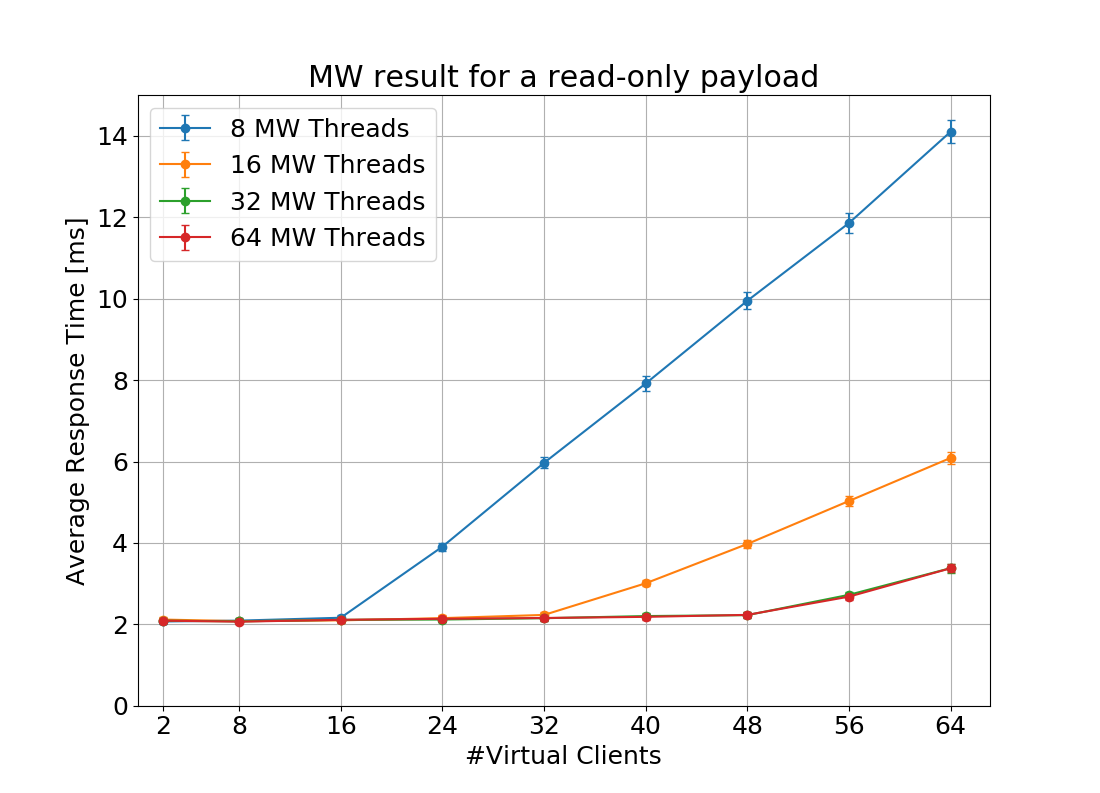
\includegraphics[width=\textwidth ]{plots/baselineWithMw/rt_ro_one_mw.png}
    \caption{Average Response Time for r-o Payload }
    \label{plt:bl:rt_ro_one_mw}
\end{subfigure}%
\begin{subfigure}{.5\textwidth}
    \centering
    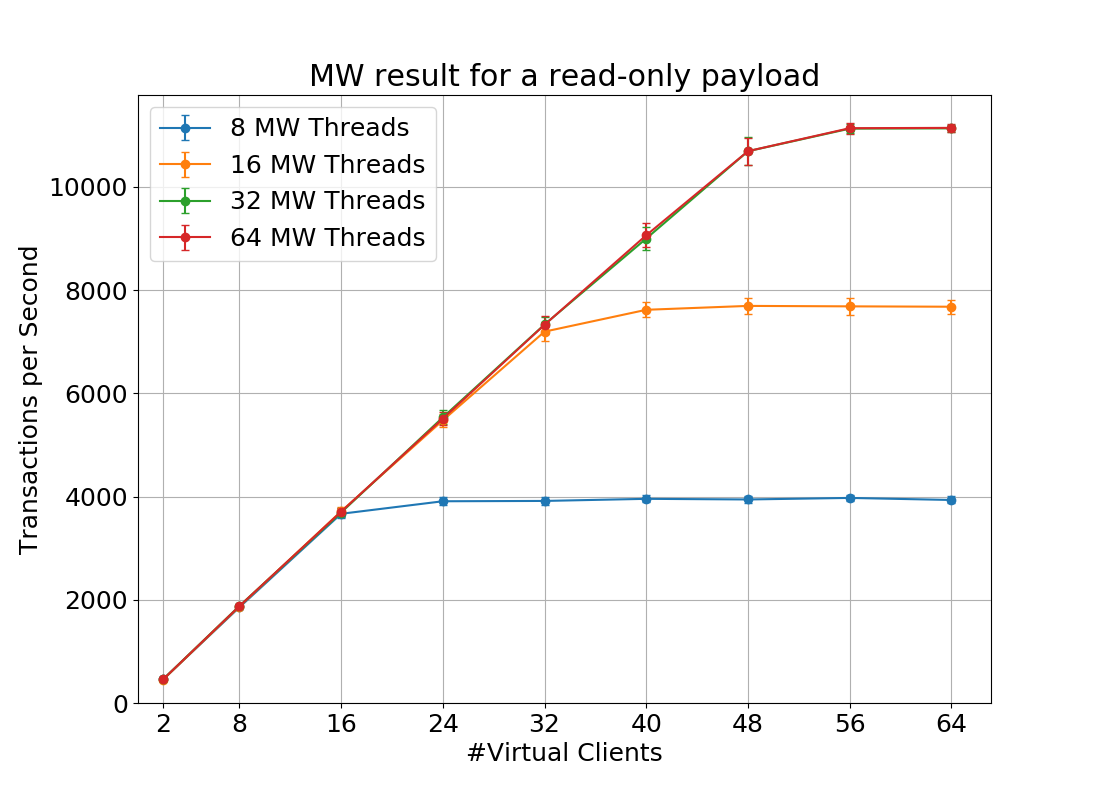
\includegraphics[width=\textwidth ]{plots/baselineWithMw/tp_ro_one_mw.png}
    \caption{Average Throughput for r-o Payload}
    \label{plt:bl:tp_ro_one_mw}

\end{subfigure}
\begin{subfigure}{.5\textwidth}
    \centering
    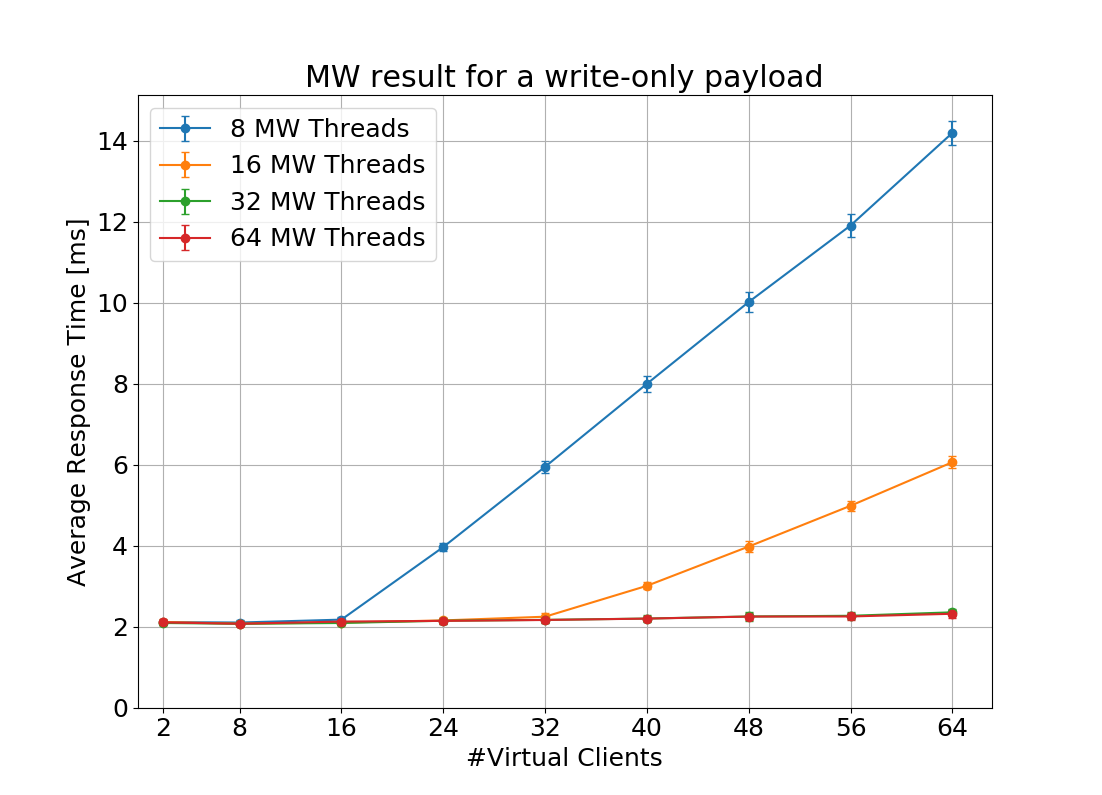
\includegraphics[width=\textwidth ]{plots/baselineWithMw/rt_wo_one_mw.png}
    \caption{Average Response Time for w-o Payload }
    \label{plt:bl:rt_wo_one_mw}
\end{subfigure}%
\begin{subfigure}{.5\textwidth}
    \centering
    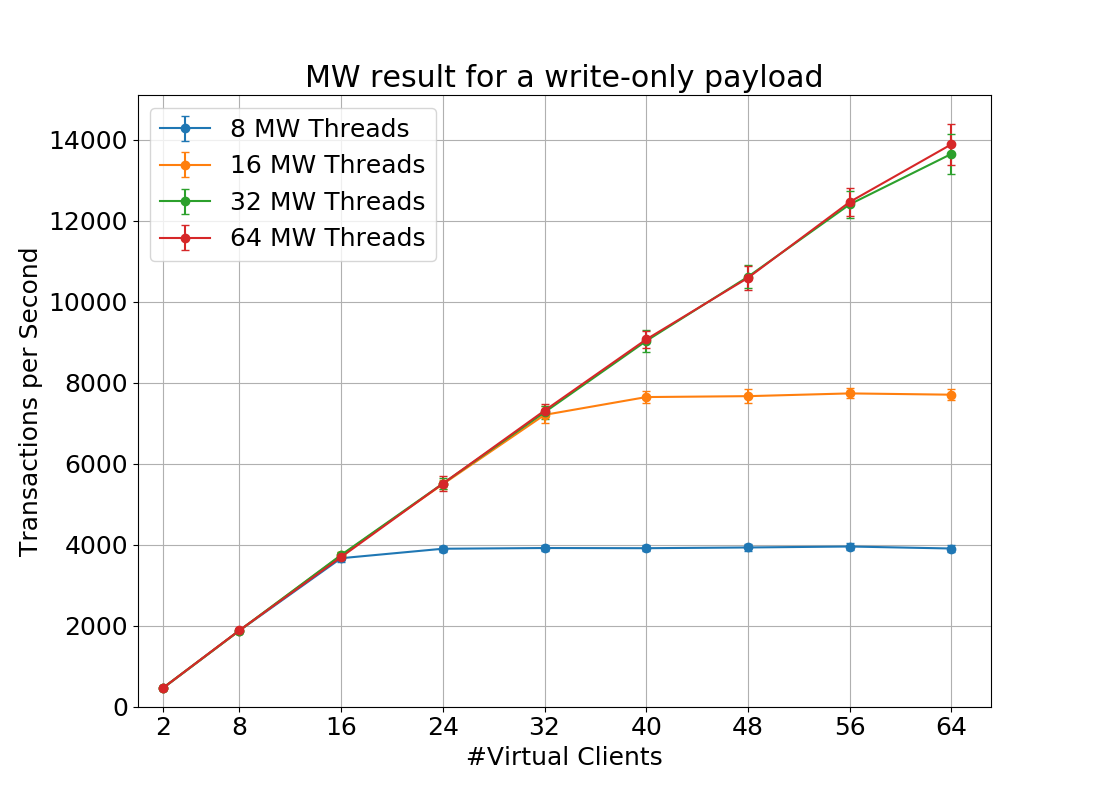
\includegraphics[width=\textwidth ]{plots/baselineWithMw/tp_wo_one_mw.png}
    \caption{Average Throughput for w-o Payload}
    \label{plt:bl:tp_wo_one_mw}

\end{subfigure}
\caption{Results for a write-only and read-only payload as measured on one middleware connected to one memtier machine and one memcached server.}
\label{plt:bl:one_mw}
\end{figure}

\begin{figure}
\centering
\begin{subfigure}{.5\textwidth}
    \centering
    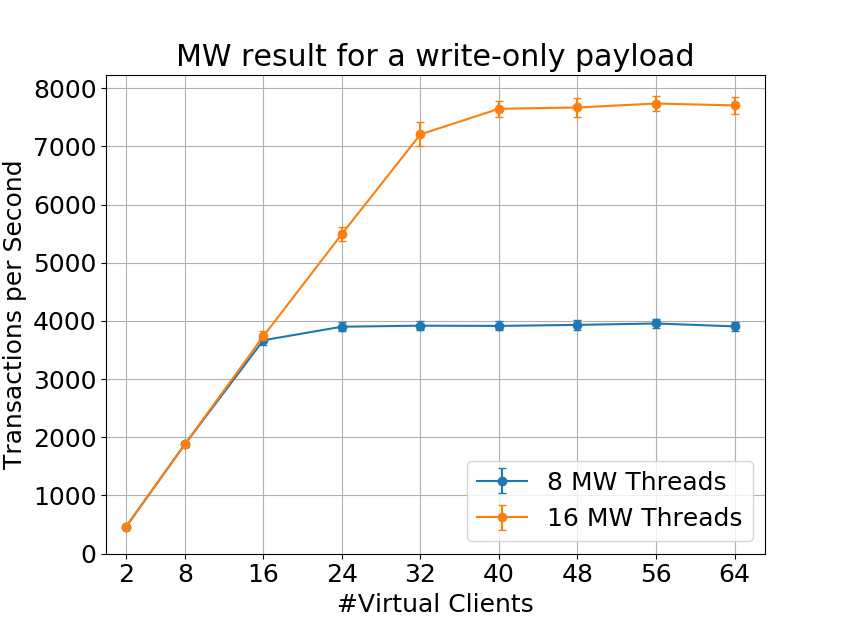
\includegraphics[width=\textwidth ]{plots/baselineWithMw/tp_start_comparison_slow.png}
    \caption{TP for 2.3 (CM) and 2.0 (MS) RTTs}
    \label{plt:bl:one_mw_comp_slow_client}
\end{subfigure}%
\begin{subfigure}{.5\textwidth}
    \centering
    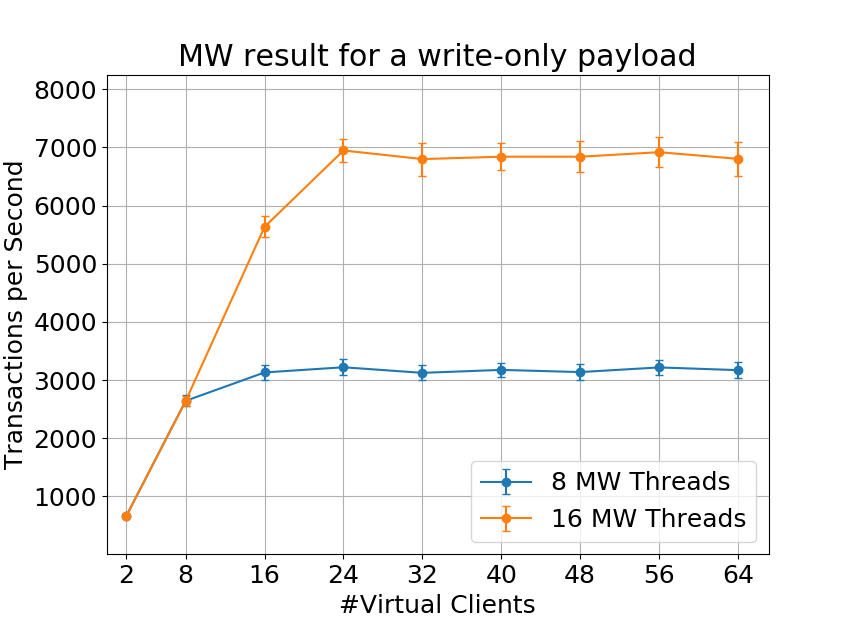
\includegraphics[width=\textwidth ]{plots/baselineWithMw/tp_start_comparison_fast.png}
    \caption{TP for 0.5 (CM) and 2.5 (MS) RTTs}
    \label{plt:bl:one_mw_comp_fast_client}

\end{subfigure}
\caption{Impact of different RTTs between client and middleware (CM) and the middleware and server (MS) on the throughput.}
\label{plt:bl:one_mw_comparison}
\end{figure}



\subsection{Two Middlewares}\label{sub:bl:two_mw}

Next we want to find out the effects of adding another middleware. Now one client is connected to each middleware by a dedicated instance and the middlewares are both connected to the same server. The parameters are again listed in the following table. Note that in order to compare to the previous experiment we did not stop the middlewares in between in order to avoid re-allocations. Furthermore, the additionally deployed MW seems to be on the same physical machine as the other MW due to the latency of 0.5 ms. This implies that it has nearly the same latencies to the server and the client as the other middleware which eases reasoning.

\begin{table}[!ht]
\begin{center}
	\scriptsize{
		\begin{tabular}{|l|c|}
			\hline Number of servers                & 1                        \\ 
			\hline Number of client machines        & 1                        \\ 
			\hline Instances of memtier per machine & 2                        \\ 
			\hline Threads per memtier instance     & 1                        \\
			\hline Virtual clients per thread       & [1 4 8 12 16 20 24 28 32]                  \\ 
			\hline Workload                         & Write-only and Read-only \\
			\hline Multi-Get behavior               & N/A                      \\
			\hline Multi-Get size                   & N/A                      \\
			\hline Number of middlewares            & 2                        \\
			\hline Worker threads per middleware    & [8 16 32 64]                  \\
			\hline Repetitions                      & 3               \\ 
			\hline Duration [sec]                      & 60              \\
			\hline 
		\end{tabular}
	} 
\end{center}
\end{table}

\paragraph{Hypothesis:} What we actually do in this experiment is splitting the same amount of clients as before over two middlewares which means we have twice as many workers as before. This means that if we now have for example 32 clients and 8 workers the throughput measured should be about twice as high as previously for 16 clients and 8 workers. This implies that our (maximal) throughputs at 64 clients is expected to be twice the throughput measured previously for 32 clients. This was 4k rps for 8 workers and 7.2k rps for 16, 32 and 64 workers. Doubling yields 8k rps for 8 workers and 14.4k rps for the others. Since with 14k rps we are again over the bandwidth limit of the server we expect the TP curves for 16, 32 and 64 workers to flatten at 11k rps for a r-o payload. Since last time for 16 workers the TP started dropping at 32 we would expect it to go up to 64 clients this time. Therefore we should not see any saturation for 16, 32 and 64 servers.
Another way to formulate it would be that the outcome of this experiment for 8 clients should look similar to the result with one MW and 16 clients (the same for 16 and 32 and so on).

\subsubsection{Explanation}
Figure \ref{plt:bl:two_mw} shows the results. From the summarized data\footnote{\url{https://gitlab.ethz.ch/siegli/asl-fall17-project/blob/master/experiment_outputs/useful/baseline_with_mw/baseline_two_mw/two-mw-plot-data.txt}} we can take away that indeed the two middlewares have very similar latency properties (ST of memcached servers and response times measured on client). As stated in the hypothesis we seem to reach the bandwidth limit of 11k rps for the r-o payload. Also do we not seem to achieve a saturated system for all number of workers but for 8 due to the reason explained in the hypothesis. However there is a slight indication that the TP starts decreasing for 32 workers at 64 clients which seems reasonable since it previously reached its TP limit at 7.5k rps. Moreover the TP for 8 workers does not completely go up to 8k rps as predicted but stops around 7.7k rps. As there is no real difference in response times measured on the client we claim that a possible reason is that we now have two instances of memtier with CT=1 each instead of one instance with CT=2. This might be less favorable for small numbers of VC. Another reason could be an increased number of connections for the server (16 instead of 8) as the curve for 8 workers is nearly identical to the curve for 16 clients from before. 


\begin{figure}[H]
\centering
\begin{subfigure}{.5\textwidth}
    \centering
    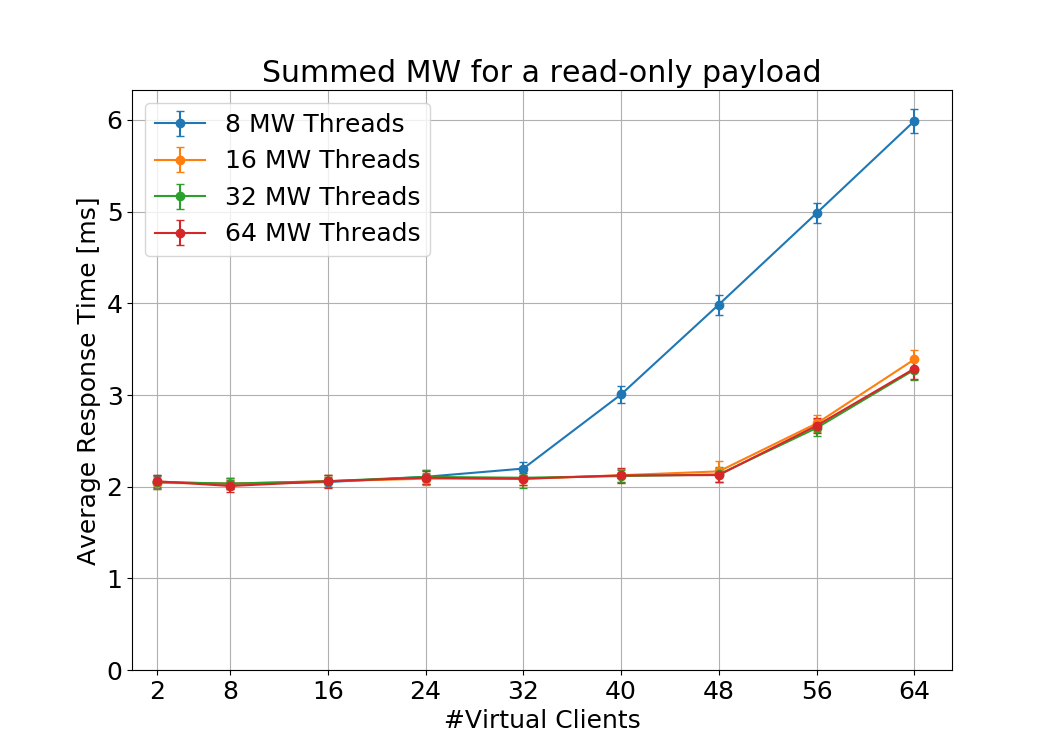
\includegraphics[width=\textwidth ]{plots/baselineWithMw/rt_ro_two_mw.png}
    \caption{Average Response Time for r-o Payload }
    \label{plt:bl:rt_ro_two_mw}
\end{subfigure}%
\begin{subfigure}{.5\textwidth}
    \centering
    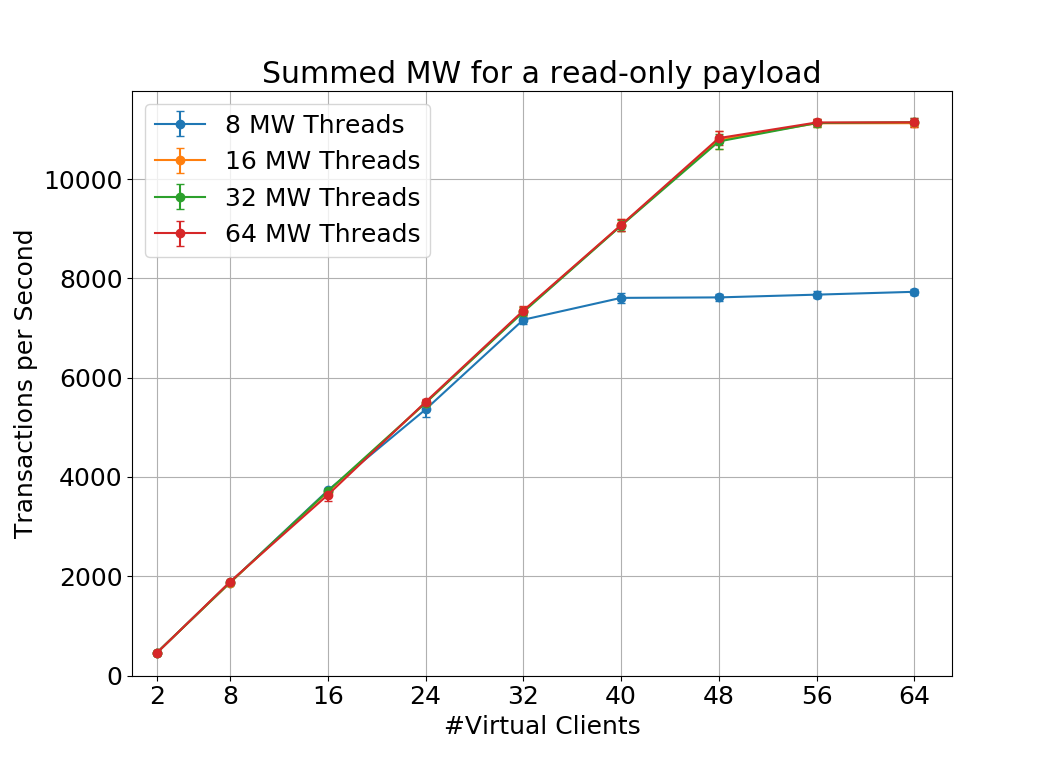
\includegraphics[width=\textwidth ]{plots/baselineWithMw/tp_ro_two_mw.png}
    \caption{Average Throughput for r-o Payload}
    \label{plt:bl:tp_ro_two_mw}

\end{subfigure}
\begin{subfigure}{.5\textwidth}
    \centering
    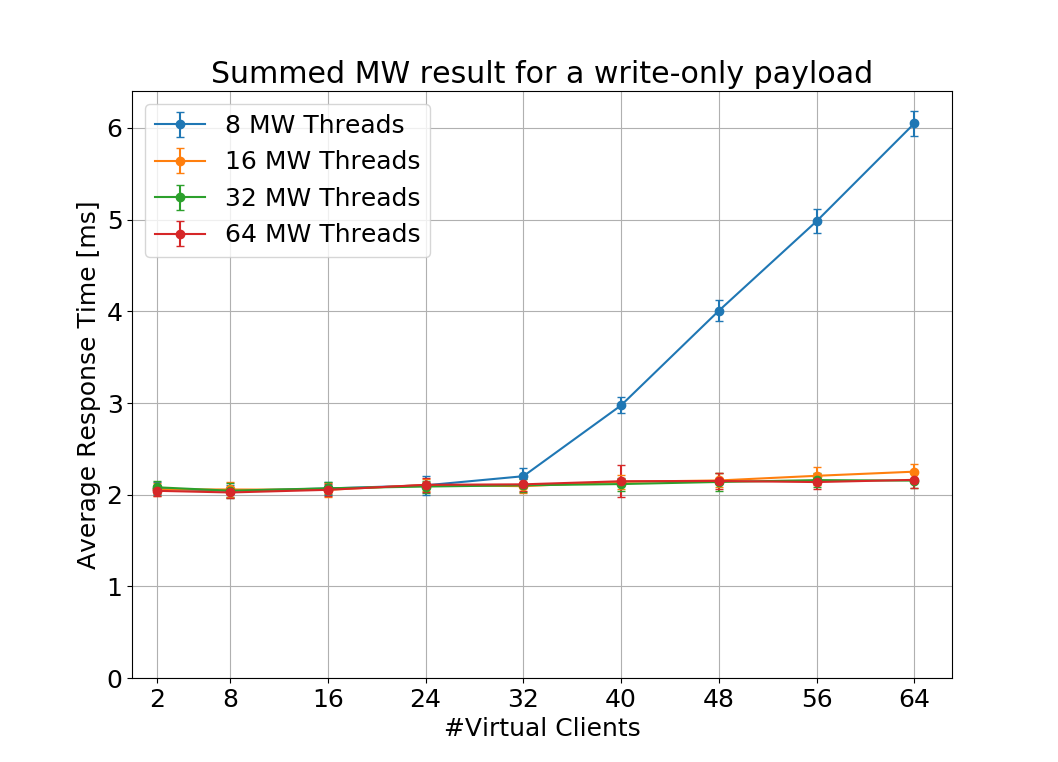
\includegraphics[width=\textwidth ]{plots/baselineWithMw/rt_wo_two_mw.png}
    \caption{Average Response Time for w-o Payload }
    \label{plt:bl:rt_wo_two_mw}
\end{subfigure}%
\begin{subfigure}{.5\textwidth}
    \centering
    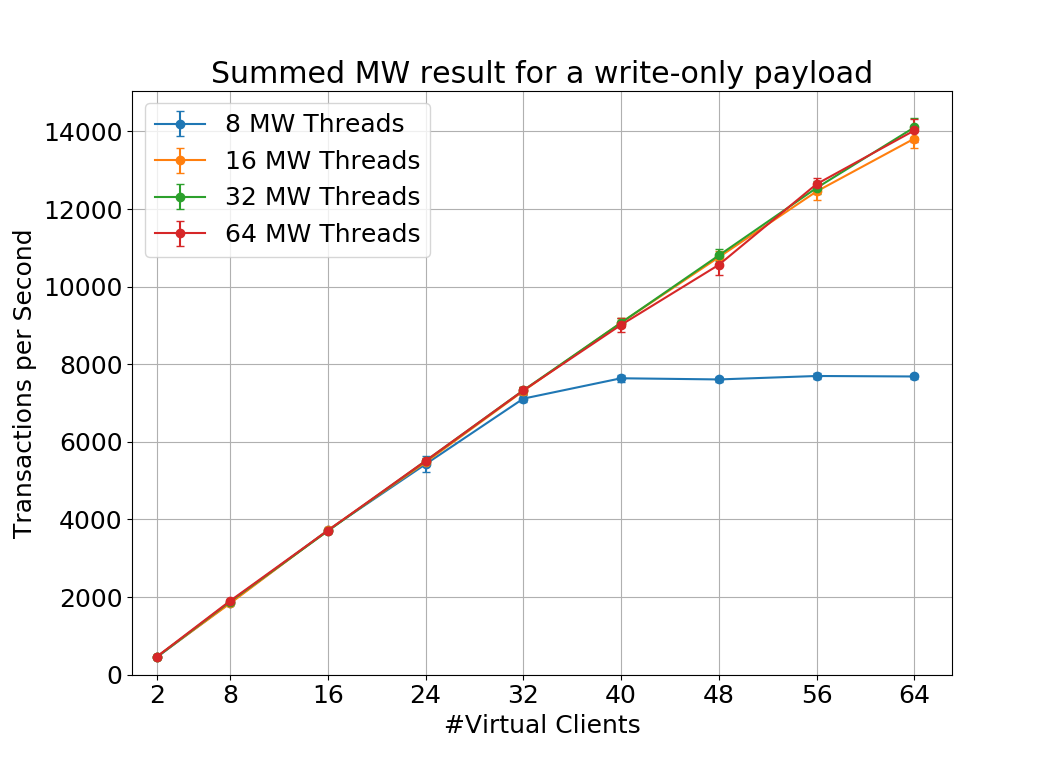
\includegraphics[width=\textwidth ]{plots/baselineWithMw/tp_wo_two_mw.png}
    \caption{Average Throughput for w-o Payload}
    \label{plt:bl:tp_wo_two_mw}

\end{subfigure}
\caption{Results for a write-only and read-only payload as measured on TWO middlewares connected to one memtier machine and one memcached server.}
\label{plt:bl:two_mw}
\end{figure}


\subsection{Heavy Load}\label{sub:heavy_load}
In order to hopefully find a saturation point for the w-o payload we conducted one last experiment. This time we used 3 load generating machines and one server both connected to one and then two middlewares. For the case with one middleware we used one memtier instance per machine (with 2 CT) and for two middlewares we used two instances with 1 CT per machine. The other parameters were chosen from the following table. In order to make the two experiments comparable we did not stop the VM's in between.

\begin{table}[!ht]
\begin{center}
	\scriptsize{
		\begin{tabular}{|l|c|}
			\hline Number of servers                & 1                        \\ 
			\hline Number of client machines        & 3                        \\ 
			\hline Instances of memtier per machine & 1 and 2                        \\ 
			\hline Threads per memtier instance     & 2 and 1                  \\
			\hline Virtual clients per thread       & 1 5 10 15 20 25 30 35 40 45 50                  \\ 
			\hline Workload                         & Write-only \\
			\hline Multi-Get behavior               & N/A                      \\
			\hline Multi-Get size                   & N/A                      \\
			\hline Number of middlewares            & 1 and 2                        \\
			\hline Worker threads per middleware    & [8 16 32 64]                  \\
			\hline Repetitions                      & 3               \\ 
			\hline Duration [sec]                      & 60              \\
			\hline 
		\end{tabular}
	} 
\end{center}
\end{table}
\begin{table}[H]

\begin{center}
	\scriptsize{
		\resizebox{0.8\textwidth}{!}{\begin{tabular}{|l||c|c|c|c|c|c|c|c|c|c|c|} \hline 
		\tb{Clients}  & \tb{6}    &      \tb{30}     &     \tb{60}       &   \tb{90}  &       \tb{120}    &     \tb{150}  &       \tb{180}     &    \tb{210}   &      \tb{240}    &     \tb{270}    &     \tb{300}     \\ \hhline{|=|=|=|=|=|=|=|=|=|=|=|=|}  
		\Xhline{4\arrayrulewidth}
		\multicolumn{12}{|c|}{\textcolor{Blue}{\tb{8 Workers}}} \\ \hline
		\multicolumn{12}{|c|}{One Middleware} \\ \hline
		TP        &     2095     &   3502    &    3490  &      3492      &  3211     &   3502    &    3515    &    3520     &   3446    &    3514     &   3492  \\ \hline
        QWT   &         0.04      &  5.57      & 14.19      & 22.71      & 34.45    &   39.57     &  48.01   &    56.39    &   65.60   &    72.38    &   81.71 \\ \hline
        ST    &         2.15     &   2.27      & 2.27    &    2.27     &   2.67     &   2.27      &  2.26    &    2.25   &     2.31    &    2.26    &    2.27 \\ \hline
        \multicolumn{12}{|c|}{Two Middlewares} \\ \hline
        TP       &      2287     &   8298   &     8189  &      8214   &     8313 &       8200   &     8260     &   8226   &     8212    &    8236    &    8252 \\ \hline
        QWT     &       0.04     &   1.08   &     4.74  &      8.43    &   11.97    &   15.82     &  19.37    &   23.19   &    26.88    &   30.50     &  34.02 \\ \hline
        ST     &        1.91     &   1.91   &     1.96   &     1.96   &     1.94    &    1.96     &   1.95     &   1.95     &   1.96   &     1.95    &    1.95 \\ \Xhline{4\arrayrulewidth}
        
        \multicolumn{12}{|c|}{\textcolor{Orange}{\tb{16 Workers}}}        \\ \hline
        \multicolumn{12}{|c|}{One Middleware} \\ \hline
        TP       &      2087   &     7076 &       7020   &     7010  &      7012  &      7015    &    7033    &    7021     &   6969    &    7025    &    6975 \\ \hline
        QWT       &     0.04     &   1.32    &    5.54     &   9.83    &   13.98     &  18.27     &  22.46     &  26.75   &    31.19    &   35.22     &  39.71 \\ \hline
        ST       &      2.15   &     2.21   &     2.26   &     2.27   &     2.26    &    2.26   &     2.26     &   2.26    &    2.28    &    2.25   &     2.28 \\ \hline
        \multicolumn{12}{|c|}{Two Middlewares} \\ \hline
        TP       &      2255    &   11651    &   15867    &   16115  &     16235   &    16162  &     16296  &     16226   &    16220    &   16185    &   16259 \\ \hline
        QWT      &      0.04    &    0.07    &    1.13    &    2.93  &      4.76   &     6.66  &      8.45   &    10.33   &    12.18    &   14.07    &   15.95 \\ \hline
        ST       &      1.93    &    1.88     &   2.00    &    1.99  &      1.97   &     1.99  &      1.97  &      1.98  &      1.98    &    1.98    &    1.98 \\ \Xhline{4\arrayrulewidth}
        
        
        \multicolumn{12}{|c|}{\textcolor{Green}{\tb{32 Workers}}}        \\ \hline
        \multicolumn{12}{|c|}{One Middleware} \\ \hline
        TP    &         2086    &   10341    &   13806    &   13935    &   13987   &    13980   &    14026   &    14034    &   14043   &    13988    &   13992 \\ \hline
        QWT    &        0.05     &   0.11    &    1.30    &    3.39    &    5.44   &     7.56   &     9.61   &    11.83   &    13.92   &    15.82   &    18.06 \\ \hline
        ST      &       2.15      &  2.10    &   2.26     &   2.27      &  2.27       & 2.27  &      2.26    &    2.26     &   2.25  &      2.26    &    2.26 \\ \hline
        \multicolumn{12}{|c|}{Two Middlewares} \\ \hline
        TP        &     2288   &    11534  &     16465   &   18489   &    20202   &    20458  &     20656   &    20696   &    20681   &    20553  &     20347 \\ \hline
        QWT       &     0.04   &     0.08    &    0.14     &   0.86   &     1.98   &     3.38   &     4.81    &    6.25   &     7.66   &     9.16   &    10.71 \\ \hline
        ST        &     1.90   &     1.89    &    2.73    &    3.20     &   3.13   &     3.12   &     3.12    &    3.10    &    3.10   &     3.12   &     3.15 \\ \Xhline{4\arrayrulewidth}
        
        \multicolumn{12}{|c|}{\textcolor{Red}{\tb{64 Workers}}}        \\ \hline
        \multicolumn{12}{|c|}{One Middleware} \\ \hline
        TP      &       2093   &    10329  &     14060  &     17010   &    20373   &    21067   &    21326  &     21518    &   21442    &   22341  &     22803 \\ \hline
        QWT     &       0.04  &      0.12  &      0.36  &      0.86   &     1.60   &     2.71   &     4.05   &     6.32    &    6.55   &     7.77  &      8.85 \\ \hline
        ST      &       2.14     &    2.10      &   2.62      &   3.17       &  2.82     &    2.82      &   2.90    &     3.64       &  2.96     &    2.85      &   2.79 \\ \hline
        \multicolumn{12}{|c|}{Two Middlewares} \\ \hline
        TP        &     2302  &     11475   &    16101  &     19201      & 21986   &    24908    &   27151   &    29136  &     29904  &     30261   &    30128 \\ \hline
        QWT       &     0.03    &    0.08   &     0.15   &     0.26      &  0.39   &     0.77  &      1.31    &    1.92  &      2.64    &    3.56    &    4.53 \\ \hline
        ST         &    1.88    &    1.89 &       2.82   &     3.50       & 4.00   &     4.16    &    4.20    &    4.15   &     4.16     &   4.16    &    4.20 \\ \hline
		\end{tabular}
		}
	} 
\end{center}
\caption{Measurements for 3 clients and one server connected to one and two middlewares. See subsection \ref{sub:heavy_load} and Figure \ref{plt:bl:one_two_middleware_3cl} for description and visualization, respectively. Note that the middleware time (MWT) has been omitted since it is mainly defined as the sum of QWT and ST. The same for QL as it is reflected by QWT.}
\label{tbl:bl:one_two_mw_comparison}
\end{table}


\subsubsection{Explanation}
For the bottleneck analysis we make use of the plots in Figure \ref{plt:bl:one_two_middleware_3cl} as well as the following two files\footnote{\url{https://gitlab.ethz.ch/siegli/asl-fall17-project/blob/master/experiment_outputs/useful/baseline_with_mw/baseline_two_mw_extended_3clients/two-mw-extended-3cl-summary-plot-data.txt}} and \footnote{\url{https://gitlab.ethz.ch/siegli/asl-fall17-project/blob/master/experiment_outputs/useful/baseline_with_mw/baseline_one_mw_extended_3cl/one-mw-extended-3cl-summary-data.txt}} which contain the data used for generating the plots amongst others such as the middleware and client measurements. We have extracted the main measurements in table \ref{tbl:bl:one_two_mw_comparison}. The two high standard deviations in Figure \ref{plt:bl:rt_one_mw_3cl} for 120 an 210 clients again arise from an outlier in a single run and can therefore be ignored.


\paragraph{One Middleware} In order to compare different worker scenarios they need to be in a saturated state. This can be read either from the plot when TP flattens or from the table when the QWT comes comes into the order of 1 ms. We notice that from 8 to 16 workers and from 16 to 32 workers the throughput doubles (e.g for 300 clients) which means the middleware seems to scale pretty well. This holds because for all three worker settings, the service times stop at roughly 2.26 ms (independent of the number of clients) while the queue waiting time is reduced by a factor of 2. As with increasing number of clients the QWT increases but the ST remains constant this means that the response time (MWT) gets mainly defined by the QWT and therefore the response time from 8 to 16 and from 16 to 32 halves and throughput doubles. Now let's look at the 64 workers scenario. We notice that the throughput does not double since $2\times 13'992 > 22'803$ despite the fact that the QWT is half so high as for 32 workers ($18.06ms \approx 2 \times 8.85ms$) so what's wrong here ? The solution is the ST which compared to 32, 16 and 8 workers rose up to 2.8 ms. 2.8 ms with 64 workers means that we can achieve at most $\frac{64req.}{2.8 ms} \approx 22.8k rps$ which we seem to hit. So now the question is why the service time increases. It could either be that our middleware has an overhead of 0.5 ms between handling 64 compared to 32 threads or it could be that the memcached server is slower due to the increased load we put on it. From section \ref{sec:bl_without_mw} we have the feeling that it could very well be the server since in Figure \ref{plt:bl:rt_one_server_1} we see that indeed the response time starts increasing in the region of 64 clients. Since we did not measure that fine-granular in section \ref{sec:bl_without_mw} and since it could also be that the memtier benchmark software has the same issues as our middleware, we conducted another baseline experiment in subsection \ref{sub:bl:memcached_latency}. Note that in between the VM's were restarted so an absolute latency comparison can not be made. By looking at the result in Figure \ref{plt:bl:one_server_two_mw} we can deduce that indeed for 64 clients the response time of memcached goes up by 0.4 ms explaining most of the 0.5 ms increasing ST. The remaining 0.1 ms could be explained with an increased overhead on the middleware e.g. increasing number of context switches compared to 32 workers as can be seen in the \tt{dstat} file\footnote{\url{https://gitlab.ethz.ch/siegli/asl-fall17-project/blob/master/experiment_outputs/useful/baseline_with_mw/baseline_one_mw_extended_3cl/dstat_mw1.txt}}. 

\paragraph{Two Middlewares} Having two middlewares with x workers should achieve the same throughput (and a bit more) as having one middleware with $2x$ workers. This due to the fact that we have the same number of connections to the server (and therefore the same ST), the same number of workers (and therefore the same QWT) but a bit less overhead because we split the workers over two machines. Hence we would expect that the curves for 32 workers and one middleware resembles the curves of 16 workers and two middlewares. From the result shown in Figure \ref{plt:bl:one_two_middleware_3cl} and in Table \ref{tbl:bl:one_two_mw_comparison} we see that this holds for 8 and 16 workers since TP doubles and RT halves. We have to mention that the additionally added middleware had a slightly fewer latency to the servers (smaller ST) and therefore the summed curves for 8 and 16 workers achieve a slightly higher throughput than previously 16 and 32 workers. For 32 workers we are below the curve of previously 64 workers. We note that the service time is with 3.15 ms about 0.3 ms higher than 2.8 with 64 workers and one MW which keeps us from reaching the 22k rps bar. Since this could also be observed in the baseline experiment without the middleware in subsection \ref{sub:bl:memcached_latency} we claim that this is not an issue of the middleware but rather of the increased memcached response time due to more traffic. Doing the bottleneck analysis for 64 workers, we see that the throughput is given by the roughly 4.2 ms service time (hence $TP = \frac{2\times64}{4.2ms} \approx 30k rps$). Since the difference in ST of roughly 2.4 ms could also be observed in the aforementioned baseline experiment (note that we now have 128 workers in total) we also make memcached responsible for being the bottleneck hindering us from doubling throughput.


\begin{figure}[H]
\centering
\begin{subfigure}{.5\textwidth}
    \centering
    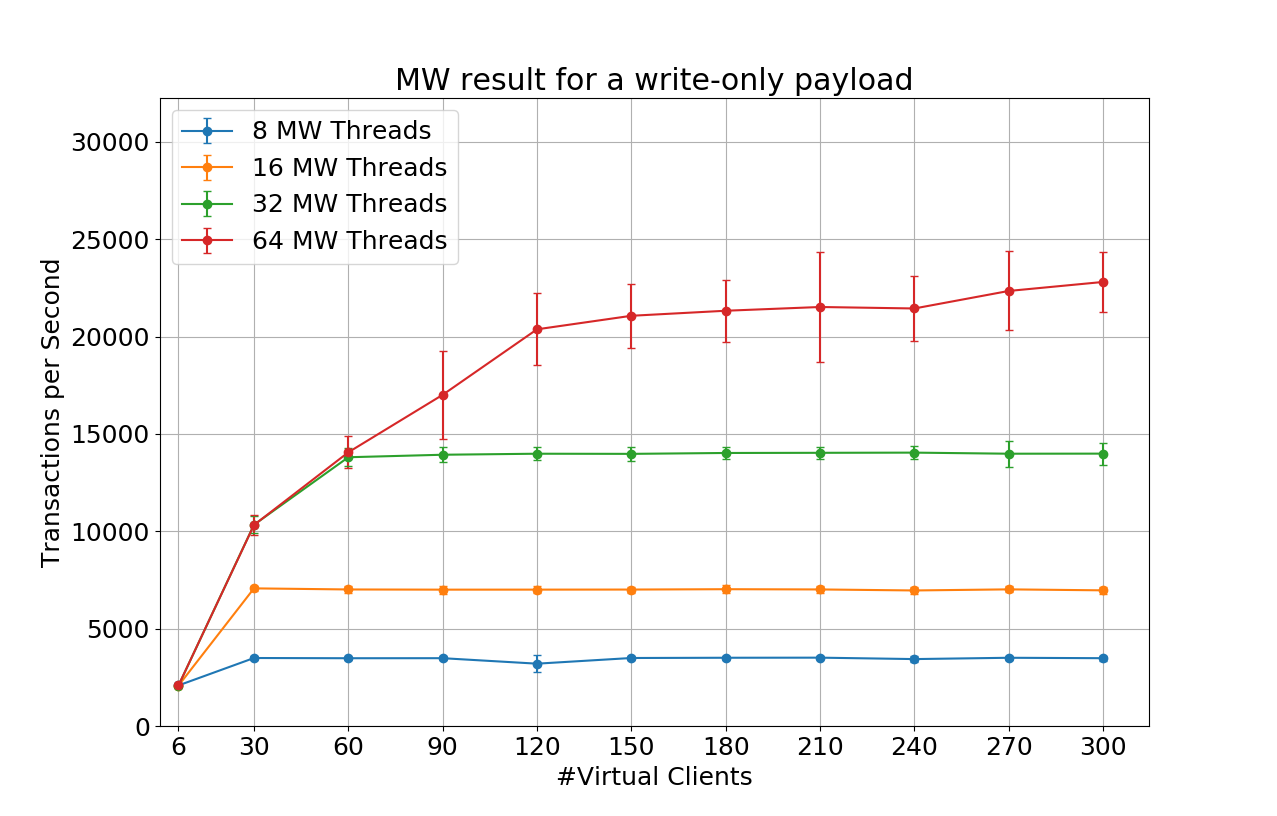
\includegraphics[width=\textwidth ]{plots/baselineWithMw/tp_one_mw_3cl.png}
    \caption{Throughput for one Middleware}
    \label{plt:bl:tp_one_mw_3cl}
\end{subfigure}%
\begin{subfigure}{.5\textwidth}
    \centering
    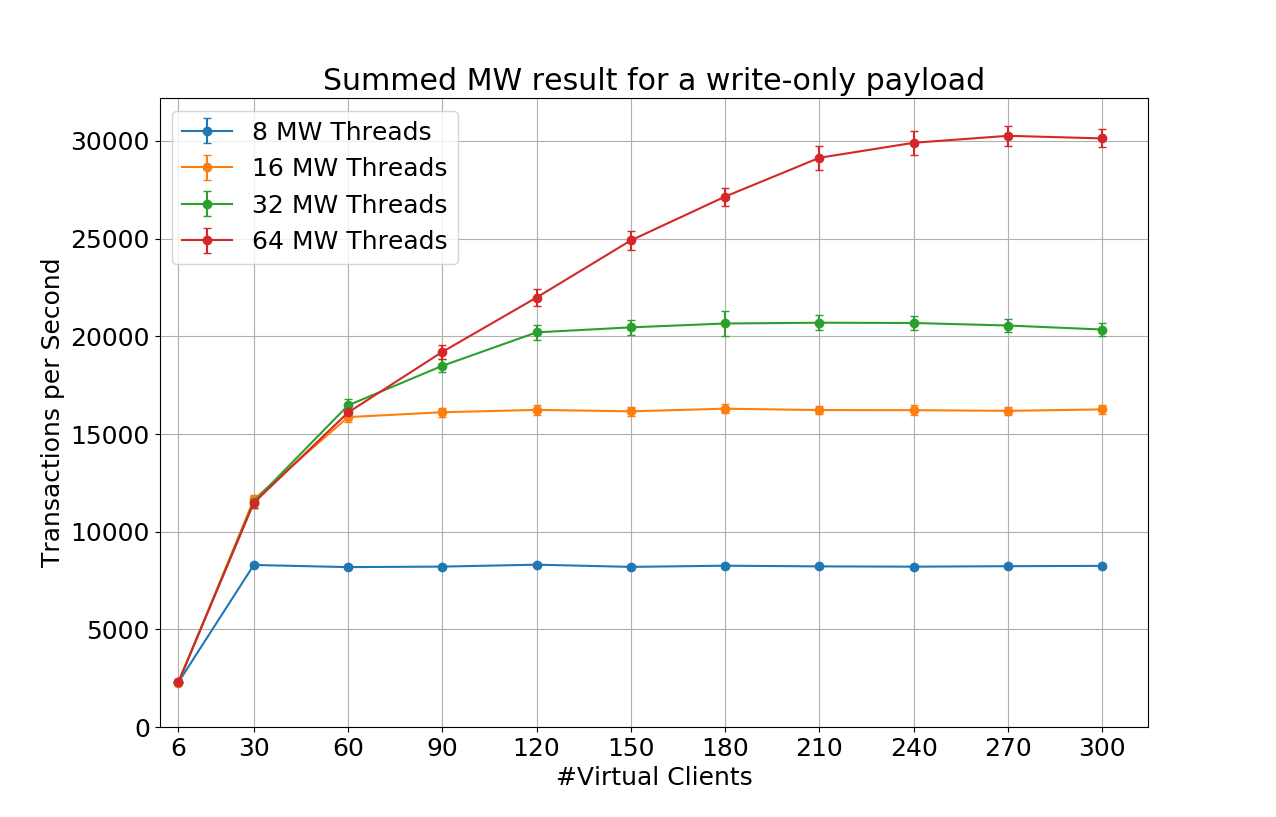
\includegraphics[width=\textwidth ]{plots/baselineWithMw/tp_two_mw_3cl.png}
    \caption{Throughput for two Middlewares}
    \label{plt:bl:tp_two_mw_3cl}

\end{subfigure}
\begin{subfigure}{.5\textwidth}
    \centering
    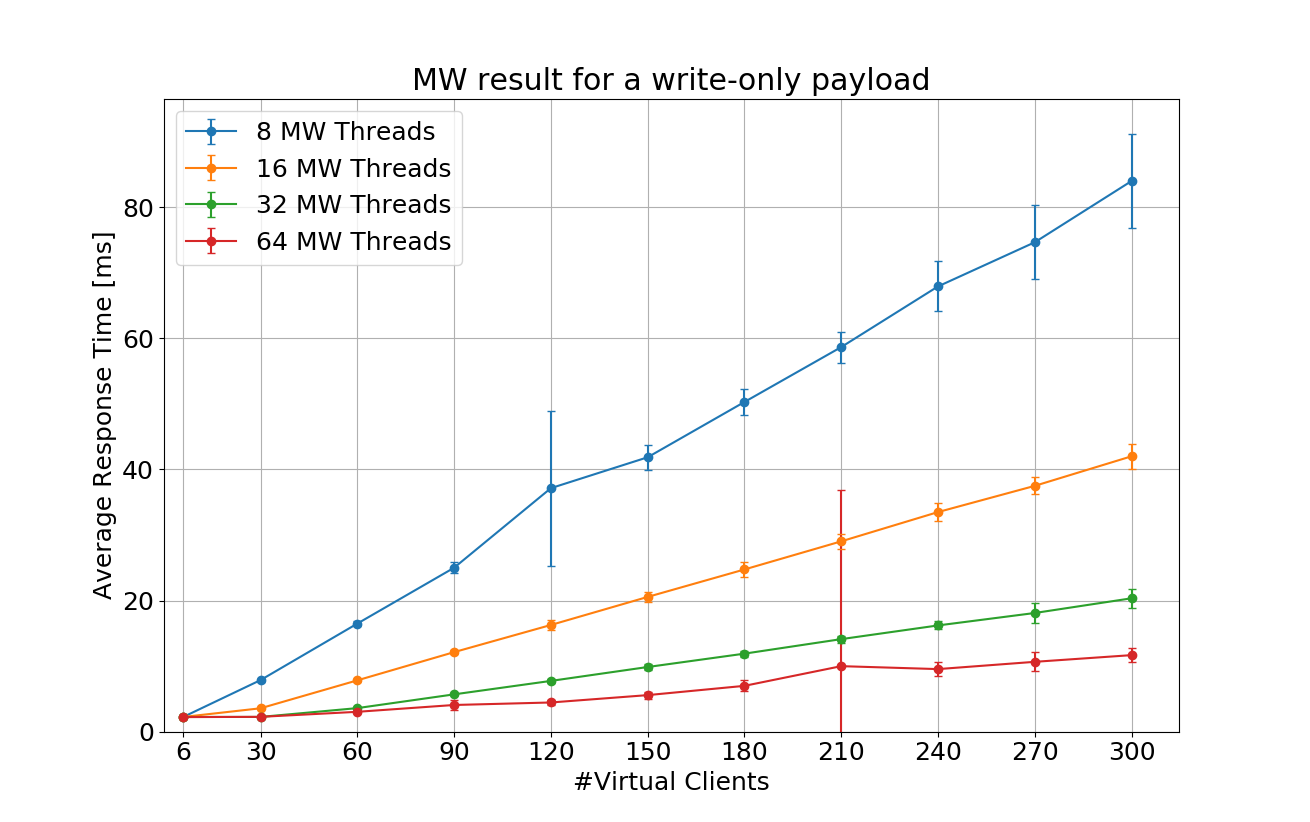
\includegraphics[width=\textwidth ]{plots/baselineWithMw/rt_one_mw_3cl.png}
    \caption{Average Response Time for one Middleware }
    \label{plt:bl:rt_one_mw_3cl}
\end{subfigure}%
\begin{subfigure}{.5\textwidth}
    \centering
    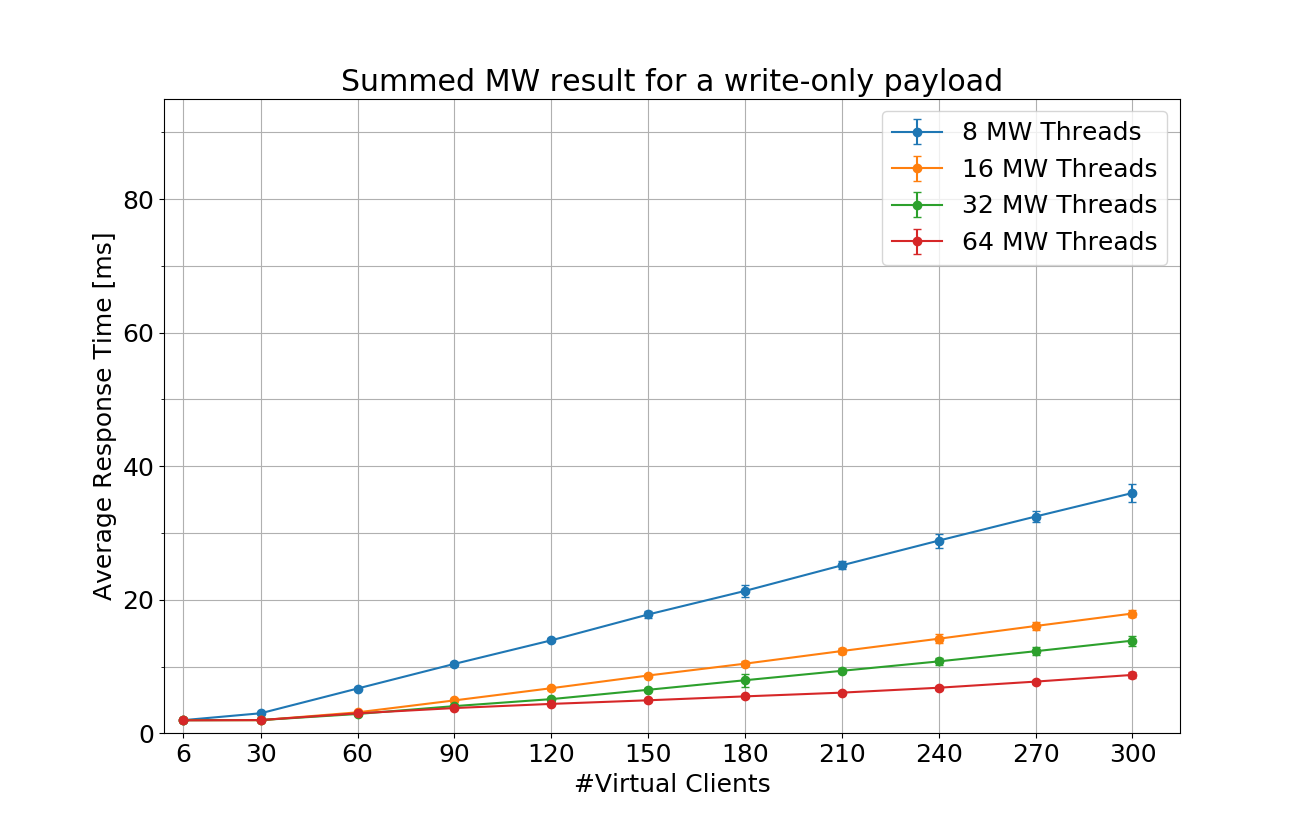
\includegraphics[width=\textwidth ]{plots/baselineWithMw/rt_two_mw_3cl.png}
    \caption{Average Response Time for two Middleware}
    \label{plt:bl:rt_two_mw_3cl}

\end{subfigure}
\caption{Result for 3 memtier and one server machines connected to one (left) and two (right) middlewares.}
\label{plt:bl:one_two_middleware_3cl}
\end{figure}


\subsection{Summary}

We use the collected data points from the previous subsections in order to fill out the following two tables. For the \ti{Reads} we will use the experiments from subsections \ref{sub:one_mw} and \ref{sub:bl:two_mw}. For the \ti{Writes} we use the information gathered in subsection \ref{sub:heavy_load}. The corresponding files can be found here\footnote{\url{https://gitlab.ethz.ch/siegli/asl-fall17-project/blob/master/experiment_outputs/useful/baseline_with_mw/baseline_one_mw/one-mw-plot-data.txt} } \footnote{\url{https://gitlab.ethz.ch/siegli/asl-fall17-project/blob/master/experiment_outputs/useful/baseline_with_mw/baseline_two_mw/two-mw-plot-data.txt} } \footnote{\url{https://gitlab.ethz.ch/siegli/asl-fall17-project/blob/master/experiment_outputs/useful/baseline_with_mw/baseline_one_mw_extended_3cl/one-mw-extended-3cl-summary-data.txt} } \footnote{\url{https://gitlab.ethz.ch/siegli/asl-fall17-project/blob/master/experiment_outputs/useful/baseline_with_mw/baseline_two_mw_extended_3clients/two-mw-extended-3cl-summary-plot-data.txt}}. In all cases we take the data for 64 workers. For the \ti{Reads} we take the point at 56 clients and for the \ti{Writes} the one for 240 clients.
\begin{table}
\begin{center}
	{Maximum throughput for one middleware.}
	\begin{tabular}{|l|p{2cm}|p{2cm}|p{2cm}|p{2cm}|}
		\hline                                & Throughput & Response time & Average time in queue & Miss rate \\ 
		\hline Reads: Measured on middleware  &     11134  &   2.68        &       0.35            &    0       \\ 
		\hline Reads: Measured on clients     &     11133  &   5.03        & n/a                   &     0      \\ 
		\hline Writes: Measured on middleware &     21442  &   9.53        &       6.55            & n/a       \\ 
		\hline Writes: Measured on clients    &     21488  &   11.25       & n/a                   & n/a       \\ 
		\hline 
	\end{tabular}
\end{center}

\begin{center} 
	{Maximum throughput for two middlewares.}
	\begin{tabular}{|l|p{2cm}|p{2cm}|p{2cm}|p{2cm}|}
		\hline                                & Throughput & Response time & Average time in queue & Miss rate \\ 
		\hline Reads: Measured on middleware  &   11140    &     2.67      &         0.20          &    0       \\ 
		\hline Reads: Measured on clients     &    11135   &     5.03      & n/a                   &    0      \\ 
		\hline Writes: Measured on middleware &   29904    &     6.83      &         2.64          & n/a       \\ 
		\hline Writes: Measured on clients    &   30073    &     8.02      & n/a                   & n/a       \\ 
		\hline 
	\end{tabular}
\end{center}
    \caption{Measurements summarizing the case for one and two middlewares.}
    \label{tbl:baseline_with_mw:measurements}
\end{table}
As the data from the \ti{Writes} and those for the \ti{Reads} were taken from two different experiments it makes not much sense to compare them against each others. Nevertheless, a short comparison between the two payloads was made in \ref{subsub:expl_one_mw}. An in depth comparison between one middleware between one middleware and two middlewares has already been made in the corresponding sections and subsection. We can say that while the r-o payloads are bandwidth bounded, the r-o are not. This results in an increasing QWT and a very low QWT for the r-o payload as the server can not catch up with the paste of the workers. For the writes we see that the QWT for two middlewares halves but throughput does not double. As mentioned in subsection \ref{sub:heavy_load} this is based on the fact that the ST of memcached increases. 



\subsection{Memcached Latency}\label{sub:bl:memcached_latency}
In order to get a more precise ground truth of the memcached service time in the view of the middlewares we conducted one more baseline experiment each of 60 seconds and over 3 runs. We used one memcached server connected to first one and then two middleware machines which run the memtier-benchmark suite. We used one memtier instance per middleware VM with CT=8 (because of the 8 virtual CPU's). By using two middleware machines we can exclude the possibility that an increasing response time arises from a phenomena inside of the benchmark software. The result is shown in Figure \ref{plt:bl:one_server_two_mw}. Interestingly, running 32 and 64 clients from 2 machines achieves a higher latency compared to running 64 and 128 from a single machine. Besides from that we see a clear effect of memcached response time depending on the load.

\begin{figure}
    \centering
    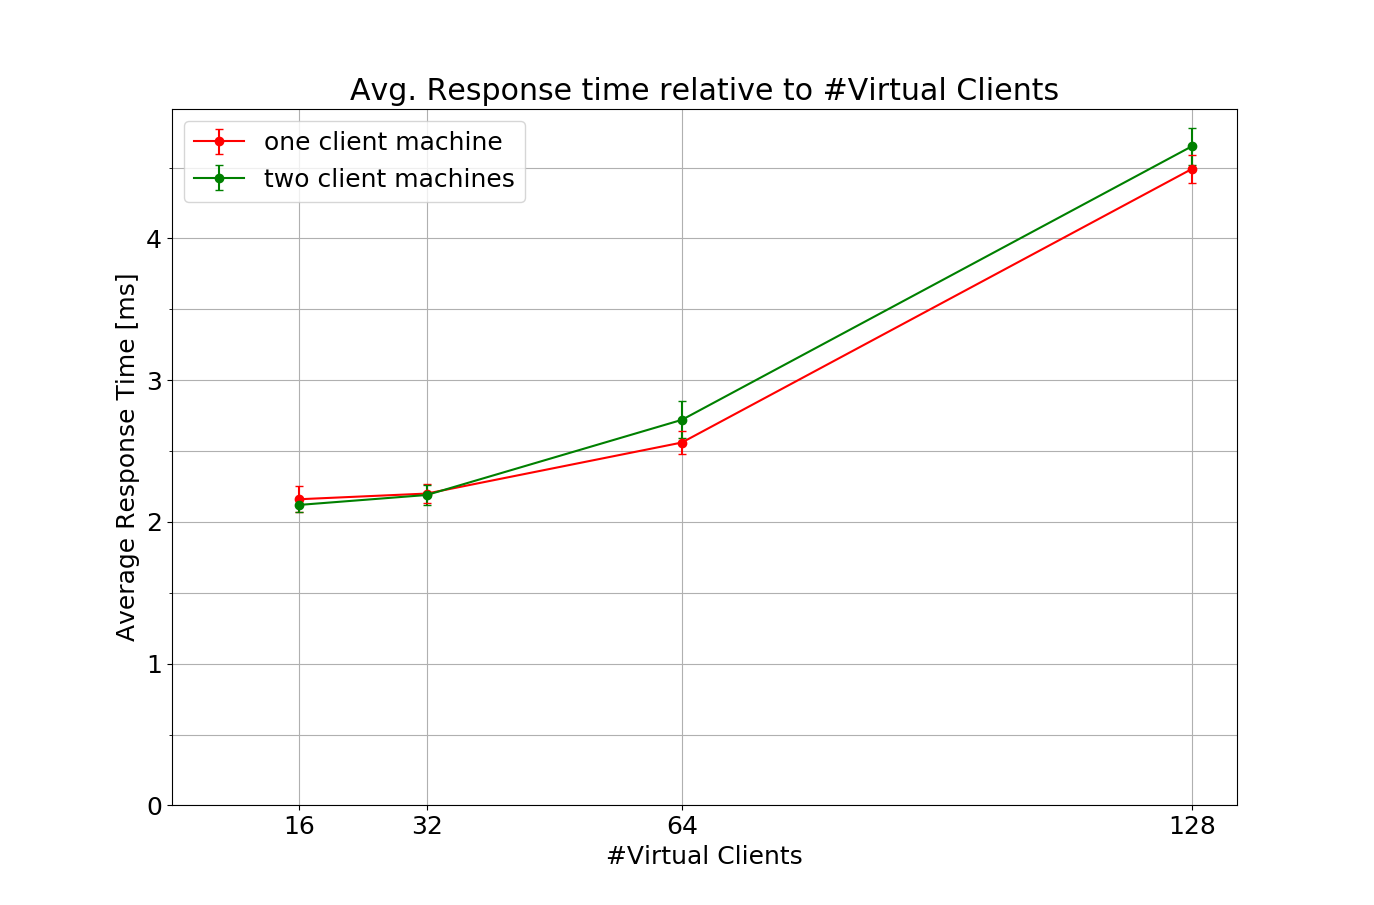
\includegraphics[width=0.7\linewidth]{plots/baselineWithoutMw/rt_one_server_from_mws.png}
    \caption{Response time of a single memcached server measured by the memtier-benchmark running on one and two middleware machines. We can see that the response time stays at 2.25 ms for up to 32 clients (=TCP connections) and then starts rising probably due to the increased load on the memcached server.}
    \label{plt:bl:one_server_two_mw}
\end{figure}





\section{Throughput for Writes (90 pts)}\label{sec:writes}

\subsection{Full System}

In order to see the effects of replicating the writes to multiple servers we run the following write-only experiment. Three load generators were connected to two middlewares which in turn were connected to three memcached servers each. We recall that each middleware worker thread has a connection to each of the three servers and forwards a SET request to all of them. We will analyze the performance depending on different number of worker threads and virtual clients. In order to be able to better compare the result to the baseline experiment in subsection \ref{sub:heavy_load} and to make sure the system gets saturated, we directly chose the number of virtual clients from the list of experiment \ref{sub:heavy_load} and also did not shoot down the virtual machines in between. The two newly added memcached server machines showed a smaller network delay to both middlewares than the already running server. This can be seen from the \tt{ping}-files and was also verified by running the memtier-benchmark tool for 60 seconds. The following table lists all experiment parameters that were considered.

\begin{center}
	\scriptsize{
		\begin{tabular}{|l|c|}
			\hline Number of servers                & 3          \\ 
			\hline Number of client machines        & 3          \\ 
			\hline Instances of memtier per machine & 2          \\ 
			\hline Threads per memtier instance     & 1          \\
			\hline Virtual clients per thread       & [1 5 10 15 20 25 30 35 40 45 50 ]    \\ 
			\hline Workload                         & Write-only \\
			\hline Multi-Get behavior               & N/A        \\
			\hline Multi-Get size                   & N/A        \\
			\hline Number of middlewares            & 2          \\
			\hline Worker threads per middleware    & [8 16 32 64]    \\
			\hline Repetitions                      & 3  \\
			\hline Duration                         & 60 seconds \\
			\hline 
		\end{tabular}
	} 
\end{center}

\subsubsection{Explanation}
The resulting throughput together with the corresponding MWT are plotted in Figure \ref{plt:writes}. Visually we can perceive that the system is saturated at 30, 60, 120 and 240 clients for 8, 16, 32 and 64 workers respectively. Additionally, compared to the baseline experiment with two middlewares in subsection \ref{sub:heavy_load} we see that there seems to be quite a performance overhead. So let's try to find out where the bottleneck is. One more time we take a look into the values gathered inside the middleware which can be found in this file\footnote{\url{https://gitlab.ethz.ch/siegli/asl-fall17-project/blob/master/experiment_outputs/useful/writes/write_throughput/writes-summary-plot-data.txt}}. When trying to explain the following main observations we always compare to the baseline experiment with two middlewares in subsection \ref{sub:heavy_load}. 

\begin{figure}[H]
\centering

\begin{subfigure}{.5\textwidth}
    \centering
    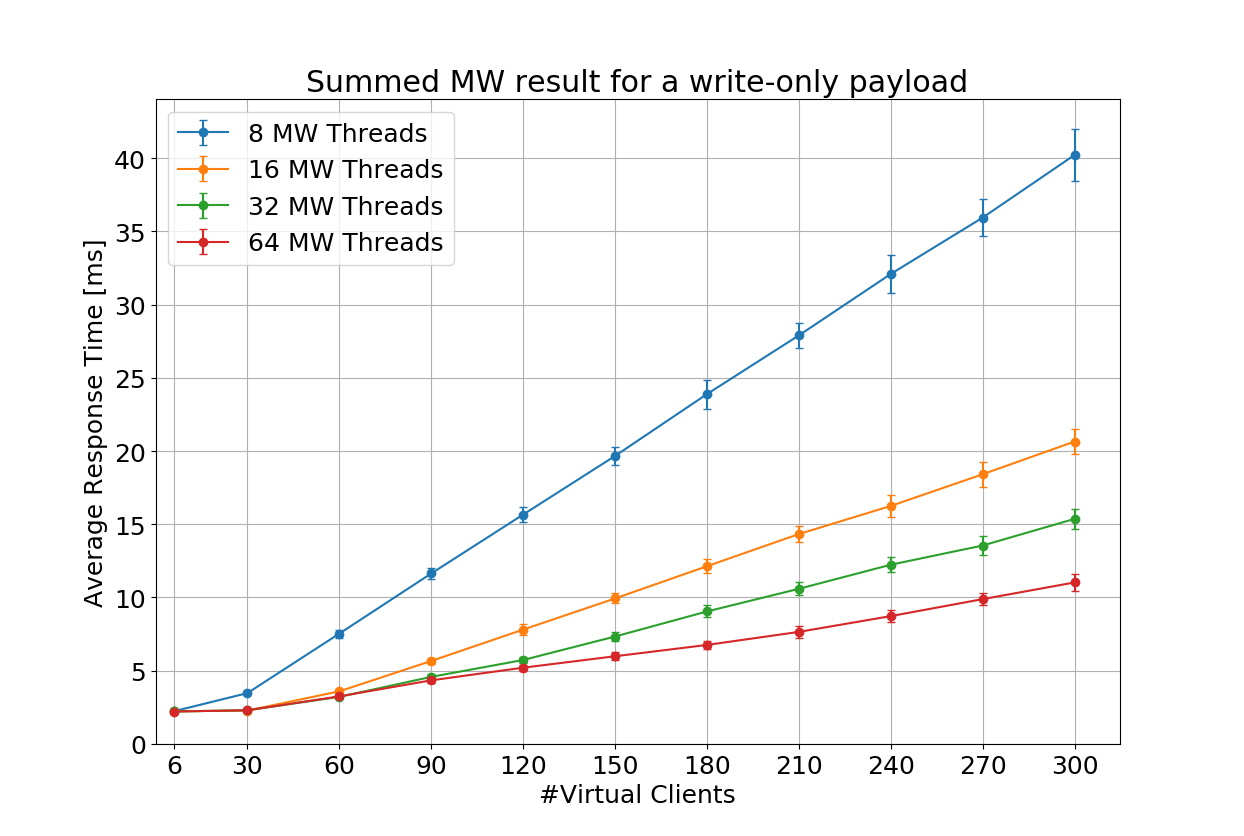
\includegraphics[width=\textwidth ]{plots/writes/rt_writes.png}
    \caption{Average Response Time for w-o Payload }
    \label{plt:write:rt}
\end{subfigure}%
\begin{subfigure}{.5\textwidth}
    \centering
    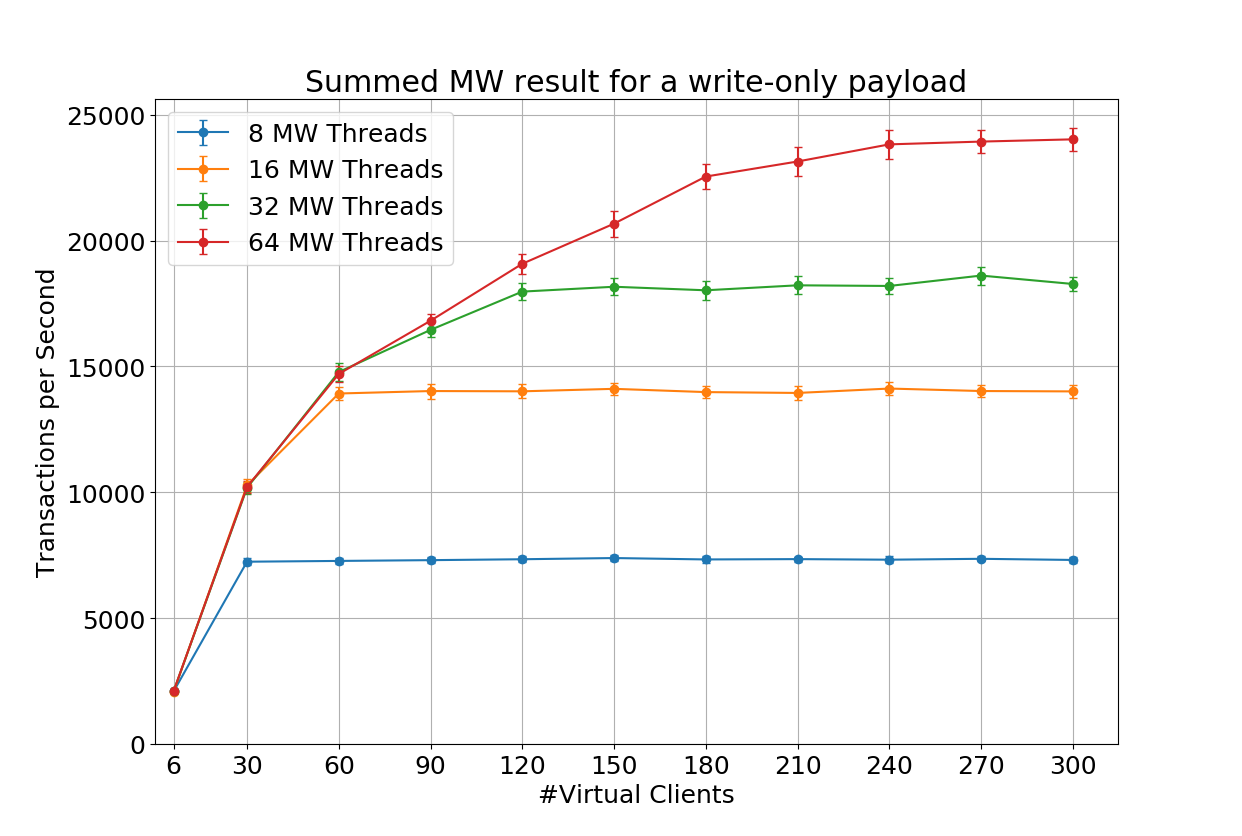
\includegraphics[width=\textwidth ]{plots/writes/tp_writes.png}
    \caption{Average Throughput for w-o Payload}
    \label{plt:write:tp}

\end{subfigure}
\caption{Results for a write-only payload as measured on two middlewares connected to three memtier machines and THREE memcached servers. The values of the SET requests are replicated to all three servers.}
\label{plt:writes}
\end{figure}


\paragraph{Service Time} The main issue seems to be the ST. Compared to the baseline this looks as follows (baseline/writeExperiment) in ms: (1.9/2.1) for 8 workers, (2.0/2.2) for 16 workers, (3.1/3.5) for 32 workers and (4.2/5.2) for 64 workers. We see that the difference increases for increasing number of workers. This service time is what defines the TP. As an example we have for 32 workers $\frac{2\times64req}{3.5ms}\approx18.2k rps$ which comes very closely to the measured 18'278 rps measured for 300 clients. As the number of connections per server for 64 workers is $\frac{3 (TCP conn.) \times 64 (workers) \times 2 (MW)}{3 (Servers)} = 2 \times 64$, the servers have the same number of TCP connections as in the baseline experiment and we cannot explain the overhead with an increase in TCP connections on the server side. A possible explanation for the increasing service time might lie in the overhead introduced from having to replicate the data values to all the servers. We recall that our definition of the service time goes from the moment we have sent the packet until we received all the responses (including parsing) therefore it could be that one server is responding slower than the one in the baseline. As mentioned at previously we measured the initial delay and can therefore exclude this possibility.  What is most likely the reason is that each worker has to receive and parse 3 responses compared to one. This comes not only with the cost of additional parsing time but also with additional system calls and therefore possible context switches since each time the worker wants to receive a response he executes a blocking read on the SocketChannel. This increase in data volume and also context switches and software interrupts can be very nicely seen in the \tt{dstat} file of the middleware(s)\footnote{\url{https://gitlab.ethz.ch/siegli/asl-fall17-project/blob/master/experiment_outputs/useful/writes/write_throughput/dstat_mw1.txt}}. An excerpt of these files is listed in Table \ref{tbl:write_overhead}. There we also see that the load goes up to 4 also indicating that there is an increasing number of processes waiting for system resources such as the network interface. Also do we observe that CPU utilization increases. Furthermore from the \tt{dstat}-file of the servers we have the confirmation that indeed they receive less traffic (26MB/s compared to 33MB/s) and that they are even more idle than in the baseline experiment. As the number of context switches is reduced with the number of workers (also visible in the \tt{dstat} file) it also makes sense that the ST overhead (listed at the beginning of this paragraph) decreases with decreasing number of workers. This also explains the fact that the throughput from 8 to 16 workers does not double.
When comparing the workers against each other we not only have the increasing context switching overheads but also the increasing memcached response time (due to more load) as could be seen in the baseline experiment. Therefore, we explain the fact that the TP does not double from 16 to 32 and from 32 to 64 workers additionally with the facts described in subsection \ref{sub:heavy_load} (Two Middlewares) and especially in \ref{sub:bl:memcached_latency}. 

\begin{table}
    \centering
    \begin{tabular}{|c|c|c|c|c|c|c|c|c|c|c|c|c|} \hline
         \multicolumn{6}{|c|}{total-cpu-usage} & \multicolumn{2}{|c|}{net/eth0} & \multicolumn{2}{|c|}{system} & \multicolumn{3}{|c|}{load-avg} \\ \hline
         usr &sys &idl &wai &hiq &siq &recv  &send &int  & csw  &1m   &5m  &15m \\ \hhline{|=|=|=|=|=|=|=|=|=|=|=|=|=|} 
         3   &8  &86  & 0  & 0 &  2 & 16M &  41M& 29k  & 39k& 4.31&2.08& 1.42 \\ \hline
          2  & 5 & 92  & 0  & 0  & 1 & 16M &  16M &21k  & 28k& 1.25& 0.99& 0.89 \\ \hline
    \end{tabular}
    \caption{Excerpt from the \tt{dstat} files of the middleware. The first row corresponds to the write-experiment of this section and the second to the baseline experiment in subsection \ref{sub:heavy_load}, both for 64 workers and 300 clients. One can clearly see an overhead introduced by the write. The reason why the outgoing data-rate is not exactly three times as high is that our throughput shrunk from 30k rps to 25k rps.}
    \label{tbl:write_overhead}
\end{table}





\subsection{Summary}\label{sub:writes:summary}

The below table shows the measurements for different number of workers taken at their maximum throughput point. As already mentioned we consider them to be at 30, 60, 120 and 240 clients for 8, 16, 32 and 64 workers, respectively. The numbers can also be found in this file\footnote{\url{https://gitlab.ethz.ch/siegli/asl-fall17-project/blob/master/experiment_outputs/useful/writes/write_throughput/writes-summary-plot-data.txt}}. For calculating the Throughput (Derived from MW response time) we applied the interactive law to the number of clients and the middleware response time but without considering the client thinking time which would roughly be the RTT between the MW and the client. Therefore this throughput is higher than the other two.
\begin{center}
	{Maximum throughput for the full system}
	\begin{tabular}{|l|p{1.5cm}|p{1.5cm}|p{1.5cm}|p{1.5cm}|}
		\hline                                            & WT=8 & WT=16 & WT=32 & WT=64 \\ 
		\hline Throughput (Middleware)                    & 7241 & 13925 & 17975 &  23826     \\ 
		\hline Throughput (Derived from MW response time) & 8645 & 16731 & 20942 &  27491     \\ 
		\hline Throughput (Client)                        & 7265 & 13955 & 17994 &  23862     \\ 
		\hline Average time in queue                      & 1.28 &  1.31 &  2.23 & 3.47      \\ 
		\hline Average length of queue                    & 3.20 &  7.01 &  14.69& 33.86      \\ 
		\hline Average time waiting for memcached         & 2.15 &  2.24 &  3.46 &  5.21     \\ 
		\hline Number of clients at max. TP point         &  30  &    60 &  120  & 240   \\
		\hline 
	\end{tabular}
\end{center}

We see that throughput measured at the client and the middleware are equal up to their standard deviation. This should be the case since anything other would indicate some kind of strange behaviour. Also do the queue lengths roughly double from each worker setting to the next. Despite also doubling the number of workers we are however not able to process process them in the same amount of time (especially for 32 and 64 workers) as can be read from the average time in queue. As analyzed in the previous subsection, this has to do with the increasing time we have to wait for memcached (ST) and the overhead of having more context switches with an increasing number of threads. As we are not able to process the requests in the same amount of time this implies that our throughput can not double for 32 and 64 workers. As this overhead usually grows non-linearly with the number of threads in the system we would expect a situation where having 2x workers does not bring any benefits or is even worse than having x workers (in terms of throughput).  


\section{Gets and Multi-gets (90 pts)}
In this section we want to test the effect of the number of keys in a GET request together with the two middleware modes (sharded / non-sharded) on the response time as measured on the clients. We use two middleware machines, each connected to three servers. Each one of the three load generating machines runs two memtier instances (with CT = 1 and VC = 2) where each instance is connected to either one of the middleware machines. For generating the multi-key payloads we use \tt{--multi-key-get=<nof\_keys>} in the \ti{memtier\_benchmark} suite. As we do not specify \tt{--ratio=<ratio>} memtier generates a default payload which also depends on the number of keys chosen before. This means it chooses a custom ratio between SET, GET and MULTIGET requests. \\
In order to better distinguish the latencies of the different request types we enhanced the middleware to keep track of the average service time for each kind separately. Besides, we introduce two more measurements: the so called \ti{Read Time (RT)} and the \ti{Number of Reads (\#R)}. The RT keeps track of the total time a thread is waiting for I/O of the response i.e. the time it waits on the blocking SocketChannel.read()\footnote{\url{https://docs.oracle.com/javase/8/docs/api/java/nio/channels/SocketChannel.html\#read-java.nio.ByteBuffer-}} method. It is therefore also contained in the service time and we can differentiate more precisely between time we wait for I/O and time we spend parsing the responses (which is the remaining part of the ST according to our chosen definition in subsection \ref{sub:timestamps}). The \#R counts how many times read() method is called per request (on average). We expect these numbers to grow with increasing number of keys per request as with an assumed Maximum Transmission Unit (MTU) of 1.5 kB (which TCP is likely to adapt its payload size to) this means we need roughly 2 TCP packets for the response of three key-values (each of size 1kB).\\
The file containing all the summarized data which will be used throughout the following discussion and which was also used for generating the graphs and tables in this section can be found here\footnote{\url{https://gitlab.ethz.ch/siegli/asl-fall17-project/blob/master/experiment_outputs/useful/reads/reads_big_latency_16workers/summary-plot-reads.txt}}. 
As we want to avoid other effects such as unnecessary context switches on the result but still have the goal to be fast enough to minimize the time a request spends in the queue, we choose the number of threads per middleware to be 16. We justify this choice with the fact that we also run the experiment with 64 threads and observed nearly identical results (very low QWT and QL) indicating that the 16 threads can cope with the total 6 clients (per MW) as well as 64 do (see summary file\footnote{\url{https://gitlab.ethz.ch/siegli/asl-fall17-project/blob/master/experiment_outputs/useful/reads/reads_big_latency_64workers/summary-plot-reads.txt}}) but bringing less overhead and therefore more stable results. Moreover, we wanted to avoid running into the bandwidth limits of the server (12.5 MBps) and therefore chose high enough network latencies from the clients to the middleware as well as from the middleware to the server. The measured total 5ms RTT from client to the server limit the maximum throughput of the 12 total clients to $\frac{12 req.}{5 ms} = 2.4k rps$ with 9 keys (of 1 KB value) this means maximal $21.6 MBps$ for all three servers and as we split the requests over three server this yields less than $12.5 MBps$ per server which means we should be fine in terms of bandwidth.


\subsection{Sharded Case}\label{sub:sharded}

In a first experiment we set the middleware into sharded mode and chose the number of keys between 1 and 12 (which should also be good regarding bandwidth). Table \ref{tbl:sharded_exp_summary} summarizes the chosen parameters.

\begin{figure}[H]
\centering

\begin{subfigure}{.5\textwidth}

\begin{center}
	\scriptsize{
		\begin{tabular}{|l|c|}
			\hline Number of servers                & 3                       \\ 
			\hline Number of client machines        & 3                       \\ 
			\hline Instances of memtier per machine & 2                       \\ 
			\hline Threads per memtier instance     & 1                       \\
			\hline Virtual clients per thread       & 2     		            \\ 
			\hline Workload                         & memtier-default             \\
			\hline Multi-Get behavior               & Sharded                 \\
			\hline Multi-Get size                   & [1 3 6 9 12]                 \\
			\hline Number of middlewares            & 2                       \\
			\hline Worker threads per middleware    & 16 \\
			\hline Repetitions                      & 3 \\
			\hline Duration                         & 60 seconds \\
			\hline 
		\end{tabular}
	} 
\end{center}
\caption{Parameters for Sharded Experiment}
\label{tbl:sharded_exp_summary}
    
\end{subfigure}%
\begin{subfigure}{.5\textwidth}
    \centering
    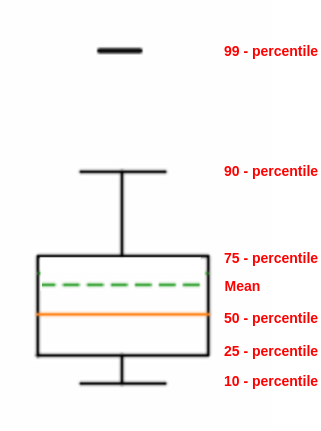
\includegraphics[width=0.43\textwidth ]{images/box_plot_legend.png}
    \caption{Legend for the Plots used in the Explanations}
    \label{fig:boxplot_legend}

\end{subfigure}
\caption{Table summarizing the parameters used in the sharded experiment together with a description of the elements used in the boxplots.}
\label{fig:boxplot_leg}
\end{figure}

As described int the design section \ref{sub:load_balancing}, when set into the sharded mode the middleware splits the keys of the initial GET request evenly over (at most) 3 new GET request each being sent to another server. Afterwards it aggregates the responses and sends one response back to the client. Requests with one key are not affected by the mode and are distributed in a round-robin manner to the servers. 

\paragraph{Hypothesis: } From the previous section \ref{sec:writes} we know that replicating requests to multiple servers and aggregating the results comes with some notable overhead. Therefore we expect to see a clear increase in latency from 1 key to 3 and more keys. Afterwards we would actually not expect to see a big increase in response time as most likely there is no big difference for memcached in serving a request with 2 keys compared with a request containing 3 keys. 


\subsubsection{Result and Explanation}
The results are shown in Figure \ref{plt:sharded_with99}. The legend explaining the meaning of the boxes can be found in Figure \ref{fig:boxplot_legend}. The plot shows the response times as measured on the clients. As we in total have 6 memtier instances (all with different latencies !) we somehow had to aggregate this data. First we looked at each instance separately and after having observed the same pattern on all instances we decided that it is okay to average them. Due to this and for visibility reasons we also do not display the standard deviations of the averages. We took advantage of the fact that memtier collects statistics for the SET and GET requests separately. Therefore whenever we talk about the average response time of a SET for example, we refer to the average of the SETs which is output at the end of the memtier run. The percentiles are then looked up in the corresponding SET-Histogram. By looking at Figure \ref{plt:sharded_with99} we also see that it makes sense to differentiate between the two requests as they seem to be affected differently and merging them would skew the result. Moreover, we notice that the distribution of the response times seems to have a long tail resulting in an average that is very close to the 75-percentile. In subsection \ref{sub:histogram} we will elaborate a bit more on the distribution.\\
\begin{figure}
\centering
\begin{subfigure}{.5\textwidth}
     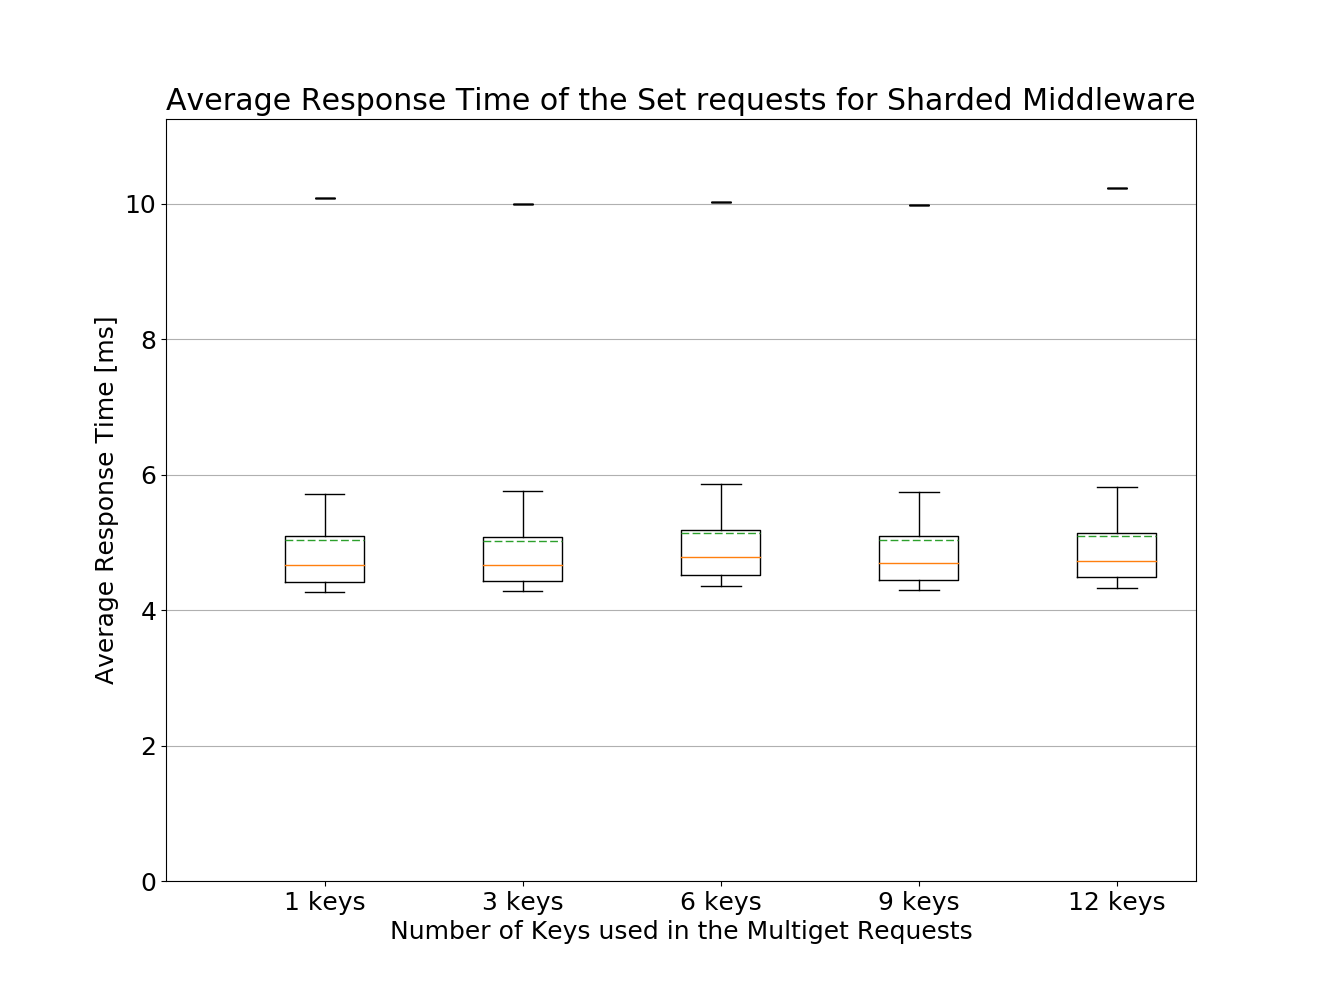
\includegraphics[width=\textwidth, trim=60 0 80 0, clip]{plots/reads/sharded_set_with99.png}
    \caption{"Sharded" SET's}
    \label{plt:sharded_set_with99}
    
\end{subfigure}%
\begin{subfigure}{.5\textwidth}
    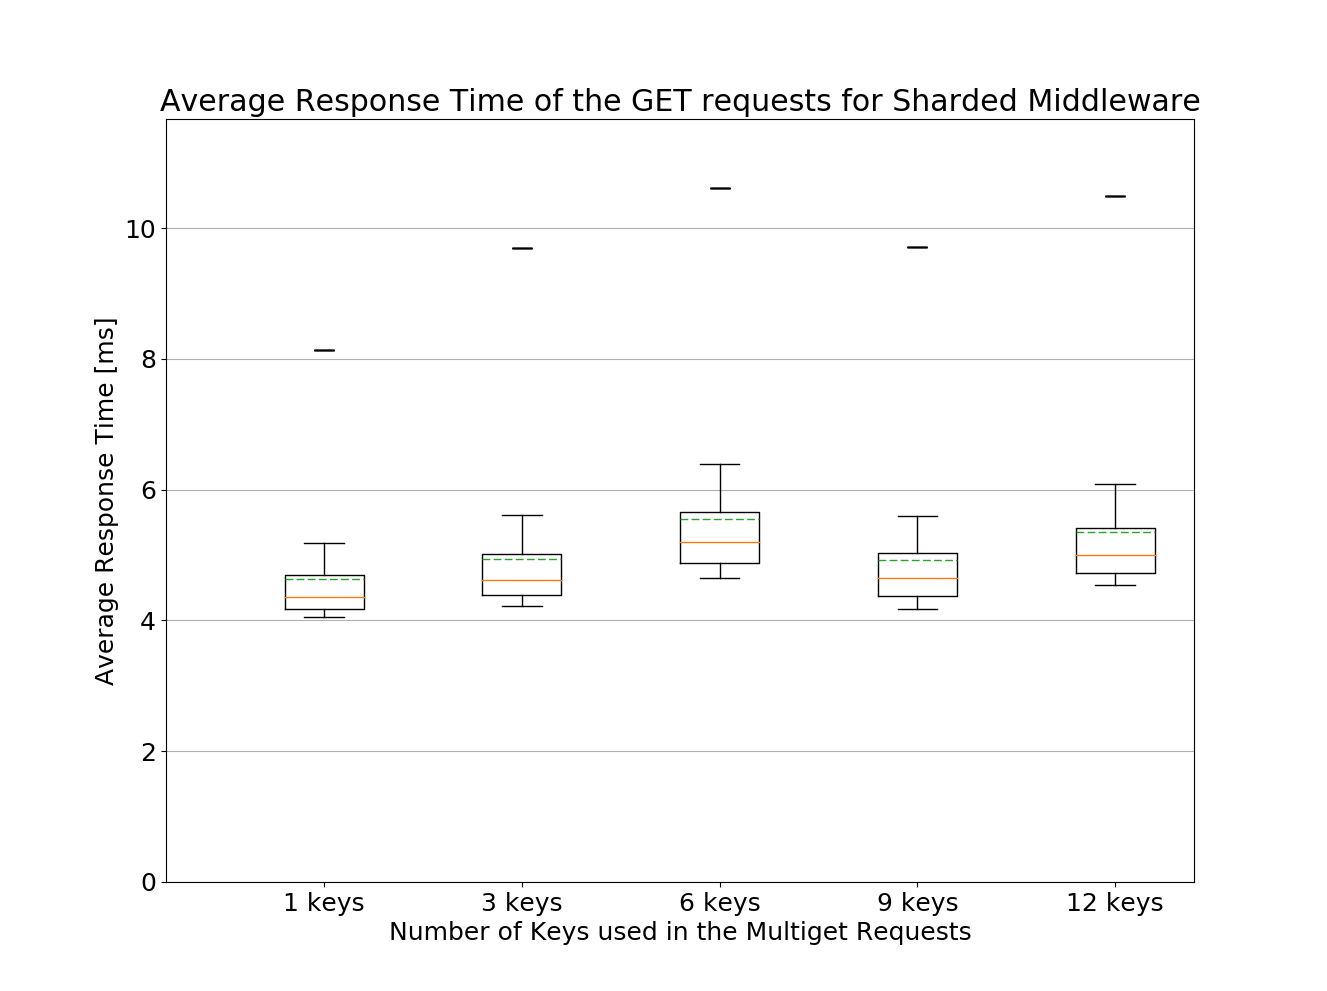
\includegraphics[width=\textwidth, trim=60 0 80 0, clip ]{plots/reads/sharded_get_with99.png}
    \caption{Sharded MULTIGETS (incl. GET)}
    \label{plt:sharded_get_with99}

\end{subfigure}
\caption{Response Times of the Sharded Middleware experiment as measured on the clients. On the left evaluated for the SET requests and on the right hand for the GET (MULTIGET inclusive) requests. Legend in Figure \ref{fig:boxplot_legend}.}
\label{plt:sharded_with99}
\end{figure}

Looking at the plots of Figure \ref{plt:sharded_with99} we state that the SET requests are not affected by the number of keys in the MULTIGET requests. This makes sense because as described in the design section they are handled separately by our middleware. This can also be seen in Table \ref{tbl:sharded_mw} showing the response times as measured on the middlewares. The SET ST stays more or less constant at 2.6 ms. Moreover we see that a MULTIGET with one key is faster  than a SET which also makes sense since the SET's are replicated to all server. Note that there is no entry for the MULTIGET ST with 1 key because they are treated as single GETs. As mentioned in the hypothesis we see in the table and from the plots that the ST for 3 keys raises to the level of the SET service times. This also makes sense since the requests are broken into 3 GET request with 1 key and distributed to all 3 servers which is very similar to what we do in the SET requests. Regarding Table \ref{tbl:sharded_mw} we see that RT $\approx$ ST which means that the service time is mainly defined by waiting on the sockets and not by (overhead such as parsing) introduced by our middleware. Focusing on the plot with the GET and MULTIGET requests we observe that the response times for 6 and for 12 keys are higher than for the others and therefore our hypothesis seems not to hold. A reason for this might be the fact that the default memtier-payload included no single GET requests in these two cases (see table) and as single GET requests (see MULTIGET with 1 key) have a shorter response time they "pull-down" the averages of the MULTIGET requests in the cases of 3 and 9 keys. This is also explaining why the measured response time at the clients for the 3-key and 9-key requests are slightly faster than the SET requests because from the middleware data (where we can differentiate the ST of GETs and MULTIGETs) we see that they are actually equally fast (2.6ms). For 12 keys we can look at the measured service time in the middlewares and indeed claim that it is only 0.1 ms higher than for 3 keys and therefore our hypothesis that there is no difference between a 3-key and a 4-key request holds. Where our explanation is not valid is for 6 keys because there also the ST on the middleware increased to 3.0 ms. This is kind of strange because there should be no such difference from sharding a 6-key request into three 2-key requests and sharding a 9-key request into three 3-key requests. A hint is given in the \#R row for the MULTIGETs. There one can see that, unlike for the other cases, with 6 keys we call read() on average 4 times per request for I/O which is highly correlating with the RT. But why is this number bigger than for e.g. 9 keys ? \\

\begin{table}
\centering
    \scriptsize{
		\begin{tabular}{|l||c|c|c|c|c|} \hline 
		\tb{Keys}  & \tb{1}    &      \tb{3}     &     \tb{6}       &   \tb{9}  &       \tb{12}   \\ \hhline{|=|=|=|=|=|=|}  
        average service time (ST)  &  2.3    &     2.5     &    2.8   &      2.5      &   2.7 \\\Xhline{2\arrayrulewidth}
        GET service time (ST)     &   2.3      &   2.2  &       0.0   &      2.2    &     0.0   \\
        GET read time (RT)   &    2.3      &   2.2      &   0.0     &    2.2     &    0.0  \\
        GET number of read calls (\#R)        &    1.0      &   1.0    &     0.0      &   1.0       &  0.0    \\\Xhline{2\arrayrulewidth}
        MULTIGET service time (ST)    &    0.0    &     2.6 &        3.0   &      2.6    &     2.7   \\
        MULTIGET read time (RT)      &  0.0      &   2.6    &     3.0     &    2.6       &  2.7  \\
        MULTIGET number of read calls (\#R)     &   0.0    &     3.0     &    4.1     &    3.0     &    3.4    \\\Xhline{2\arrayrulewidth}
        SET service time (ST)   &     2.7     &    2.6      &   2.6     &    2.6   &      2.6   \\
        SET read time (RT)     &  2.6      &   2.6     &    2.6     &    2.6     &    2.6   \\
        SET number of read calls (\#R)    &    3.0      &   3.0    &     3.0      &   3.0     &    3.0 \\\Xhline{2\arrayrulewidth}
        MULTIGET length  &            0    &       3    &       5      &     9      &    10 \\\Xhline{2\arrayrulewidth}
        number of GET requests per second   &  2393    &     499   &        0   &      836     &      0 \\
        number of MULTIGET requests per second&  0    &    1497    &    1549   &      836     &   1201  \\
        number of SET requests per second  &   239     &    499     &    774   &      836      &  1201 \\ \hline

		\end{tabular}
	}
    \caption{Response times in milliseconds as measured on the two middlewares (averages) when put into sharded mode.}
    \label{tbl:sharded_mw}
\end{table}

In order to find out whether this has to do with our middleware or not we run the memtier-benchmark from one middleware machine to one (populated) memcached server first with 2 MULTIGET keys and then with 3 MULTIGET keys. Note that the average multiget key size in the default memtier payload for 6 keys was 5 keys which means server1 and server2 got a 2-key GET request and server3 a single GET request. The parameters used for 3 keys were\tt{ --multi-key-get=3 --ratio=0:3}. The summarized data over 3 runs of 60 seconds is illustrated in Figure \ref{plt:reads:comp_2_3_keys} and the corresponding data can be found in this file\footnote{\url{https://gitlab.ethz.ch/siegli/asl-fall17-project/blob/master/experiment_outputs/useful/reads/multiget_2keys_comp/summary-plot-reads.txt}}. Indeed, we see that for 3 keys the resulting response time is on average 0.4 ms smaller than for 2 keys. Furthermore does the distribution look more dense which is a sign for more stability. As we have generated "pure" MULTIGET payloads this can not come from single GETs. We digged a bit deeper and used \tt{wireshark}\cite{wireshark} in conjunction with \tt{tcpdump} (\tt{ssh mw1 "sudo tcpdump -s0 -w -" | wireshark -k -i -}) in order to capture and display the requests sent in a \tt{telnet} session from the middleware to the server. Figure \ref{img:wires1hark_caption} shows the caption. The packets which are ignored (grey) correspond to TCP-\ti{ACKs}. Even if it is only a single sample we can observe that the overall response time for 2 keys was 2.9 ms and for 3 keys 2.3 again underlining the result of the memtier experiment. Moreover, we note that for 3 keys the time between the first and the last response packet is only 0.1 ms whereas for 2 keys we measured 0.6 ms. This is a possible explanation why we measured more read calls on the middleware (\#R in table \ref{tbl:sharded_mw}) because the workers are woken up twice by the operating system signaling an I/O event. We can only speculate over the reason for this phenomena. It might be an issue in memcached but even likely of the virtual network and therefore out of our control. As we could observe this effect in different settings especially without having the middleware involved, we claim that it has nothing to do with the implementation or the design of our middleware. From now on we will refer to the phenomena as the \ti{misty-2keys-effect}.\\


Summarizing the sharded mode we can say that our hypothesis could be verified except for 6 keys. This means that single GETs are fastest followed by the remaining cases. This can be seen from the service times inside the middleware. The fact that on the clients we measured a higher response time for 12 keys is because the default memtier payload included no single GET requests. For the behaviour of the 6 keys we make the misty-2keys-effect responsible for the higher service times on the middlewares resulting in a higher response time on the clients.

\begin{figure}
\begin{subfigure}[b]{.3\textwidth}
    \centering
    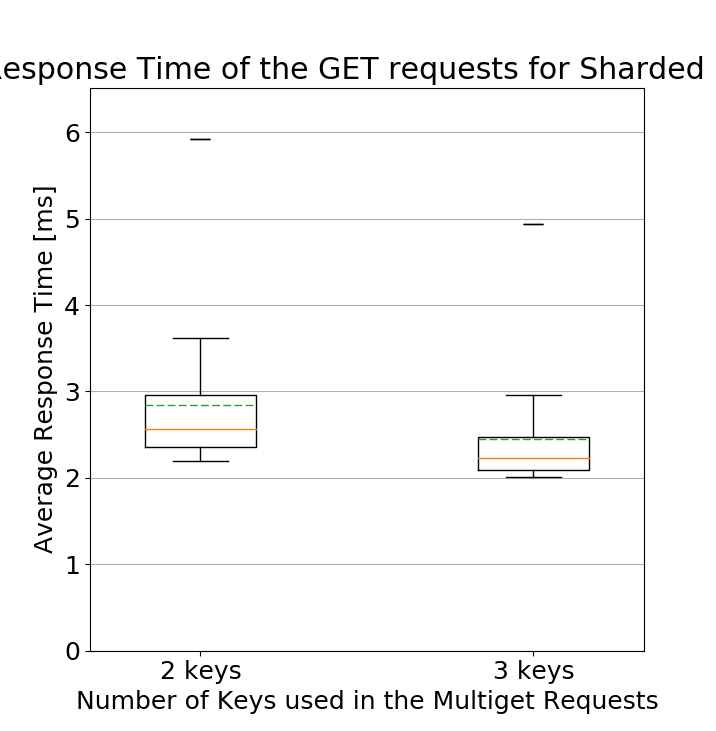
\includegraphics[width=\textwidth, trim=0 0 0 60, clip]{plots/reads/comp_2_3_keys.png}
    \caption{Memtier Experiment Result}
    \label{plt:reads:comp_2_3_keys}
\end{subfigure}%
\begin{subfigure}[b]{.7\textwidth}
    \centering
    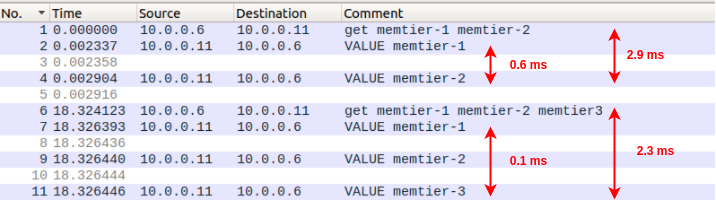
\includegraphics[width=\textwidth]{images/wireshark_capture.png}
    \caption{Wireshark Caption}
    \label{img:wires1hark_caption}
\end{subfigure}%
\caption[lof caption]{Result of comparing a 2-key MULTIGET to a 3-key MULTIGET. On the left as measured by memtier during a 60 second test run with 3 repetitions and on the right as captured by \tt{wireshark} in a \tt{telnet} session. The original caption can be found here\footnote{\url{https://gitlab.ethz.ch/siegli/asl-fall17-project/blob/master/experiment_outputs/useful/reads/multiget_2keys_comp/wireshark_caption_1_5_9_keys.pcapng}}.}
\label{img:reads:comp23}
\end{figure}


\newpage

\subsection{Non-sharded Case}\label{sub:non_sharded}

In this subsection we want to see the differences of the previous result when the middlewares are set into non-sharding mode. The remaining parameters were chosen like in the sharded case according to the following table.

\begin{center}
	\scriptsize{
		\begin{tabular}{|l|c|}
			\hline Number of servers                & 3                       \\ 
			\hline Number of client machines        & 3                       \\ 
			\hline Instances of memtier per machine & 2                       \\ 
			\hline Threads per memtier instance     & 1                       \\
			\hline Virtual clients per thread       & 2                		 \\ 
			\hline Workload                         & memtier-default             \\
			\hline Multi-Get behavior               & Non-Sharded             \\
			\hline Multi-Get size                   & [1 3 6 9]                  \\
			\hline Number of middlewares            & 2                       \\
			\hline Worker threads per middleware    & 16 \\
			\hline Repetitions                      & 3    \\
			\hline Duration                         & 60 seconds \\
			\hline 
		\end{tabular}
	} 
\end{center}

\paragraph{Hypothesis: }
As this time the number of keys in one request sent to the server is increased, we expect the response times to increase from 1 up to 12 keys. This because we have more TCP packets that need to be exchanged coming at the cost of additional packet processing on the network interfaces and also switching/routing overhead in the network. As mentioned previously, for every additional 3 keys in a request we estimate to receive two more TCP segments as response due to the MTU of 1.5 kB. Actually this could also be verified in the \tt{wireshark} caption seen in the subsection before. Other effects with more keys could be a longer look-up time on the server. Due to these reasons we would expect a longer RT (and therefore also service time) on the middleware and also a higher number of read calls (\#R).


\subsubsection{Results and Explanation}
Figure \ref{plt:non_sharded_get_with99} and Table \ref{tbl:non_sharded_mw} visualize and summarize the data gathered on the clients and in the middleware, respectively. This time we omitted the box plot for the SET requests as it looks nearly the same as in the sharded case which is what we would expect since the SET requests are still handled separately by our middleware. Looking at the middleware table we can also verify that for the SET requests nothing changed and they still have a response time of 2.6 ms. By further looking at the table we see that our hypothesis seems to hold. Not only did we measure a higher service time for higher number of keys but also did the \#R values increase. Generally, this time the \#R values are lower because we do not have to wait for the responses of all three servers but only from one which results in shorter inter-arrival times (and therefore less I/O calls) of the response segments. The differences in averaged service times on the middleware do, likewise in the sharded case, pretty much reflect what we measure on the clients. This should always hold and just servers as a basic sanity check. As previously, the default memtier payloads for 6 and 9 keys did not contain any single GET requests and therefore the average ST and the response time measured on the clients are harder to compare for different keys. For example do we measure the same response times for 6  and 9 keys but this is only because we have different payloads. Therefore when comparing the response times of the MULTIGET requests we should always consider the MULTIGET ST measured on the middlewares. By looking at the \tt{dstat} files of the servers\footnote{\url{https://gitlab.ethz.ch/siegli/asl-fall17-project/blob/master/experiment_outputs/useful/reads/reads_big_latency_16workers/dstat_server1.txt}} we can also exclude the possibility that the increased ST arise from a limiting bandwidth as the maximal throughput we achieve with 12 keys is roughly 8 MBps per server which is below the 12.5 MBps limit.
Summarizing we can say that our hypothesis holds which means that the service times of the MULTIGET requests increase with increasing number of keys due to the reasons mentioned in the hypothesis. A small exception seems to be the case with 3 keys as it achieves the same response time as the 1-key requests possibly also due to the mixed payload.


\begin{table}
\centering
    \scriptsize{
		\begin{tabular}{|l||c|c|c|c|c|} \hline 
		\tb{Keys}                           & \tb{1}    &      \tb{3}     &     \tb{6}       &   \tb{9}  &       \tb{12}   \\ \hhline{|=|=|=|=|=|=|}  
        average service time (ST)           &  2.3     &    2.4     &    2.5    &     2.5    &     2.8 \\\Xhline{2\arrayrulewidth}
        GET service time (ST)               &   2.3    &     2.3   &      0.0   &      2.3   &      0.0   \\
        GET read time (RT)                  &    2.3   &      2.2   &      0.0  &       2.2  &       0.0  \\
        GET number of read calls (\#R)      &  1.0     &    1.0     &    0.0    &     1.0    &     0.0    \\\Xhline{2\arrayrulewidth}
        MULTIGET service time (ST)          &    0.0   &      2.3   &      2.5  &       2.7  &       2.9   \\
        MULTIGET read time (RT)             &  0.0     &    2.3     &    2.5    &     2.7     &    2.9  \\
        MULTIGET number of read calls (\#R) &   0.0    &     1.0    &     1.5   &      1.9    &     2.4    \\\Xhline{2\arrayrulewidth}
        SET service time (ST)               &    2.7   &      2.6   &      2.6  &       2.6  &       2.6   \\
        SET read time (RT)                  &   2.7    &     2.6    &     2.6    &     2.6    &     2.6 \\
        SET number of read calls (\#R)      &  3.0     &    3.0      &   3.0    &     3.0      &   3.0\\\Xhline{2\arrayrulewidth}
        MULTIGET length                     &   0     &    3    &       5      &     9      &    10 \\\Xhline{2\arrayrulewidth}
        number of GET requests per second             &  2385   &      519    &       0   &      827   &        0 \\
        number of MULTIGET requests per second   &     0   &     1557    &    1654    &     827   &     1180\\
        number of SET requests per second               & 238    &     519     &    827      &   827     &   1180 \\ \hline

		\end{tabular}
	}
    \caption{Response times in milliseconds as measured on the two middlewares (averages) when put into sharded mode.}
    \label{tbl:non_sharded_mw}
\end{table}

\begin{figure}[H]
\centering
    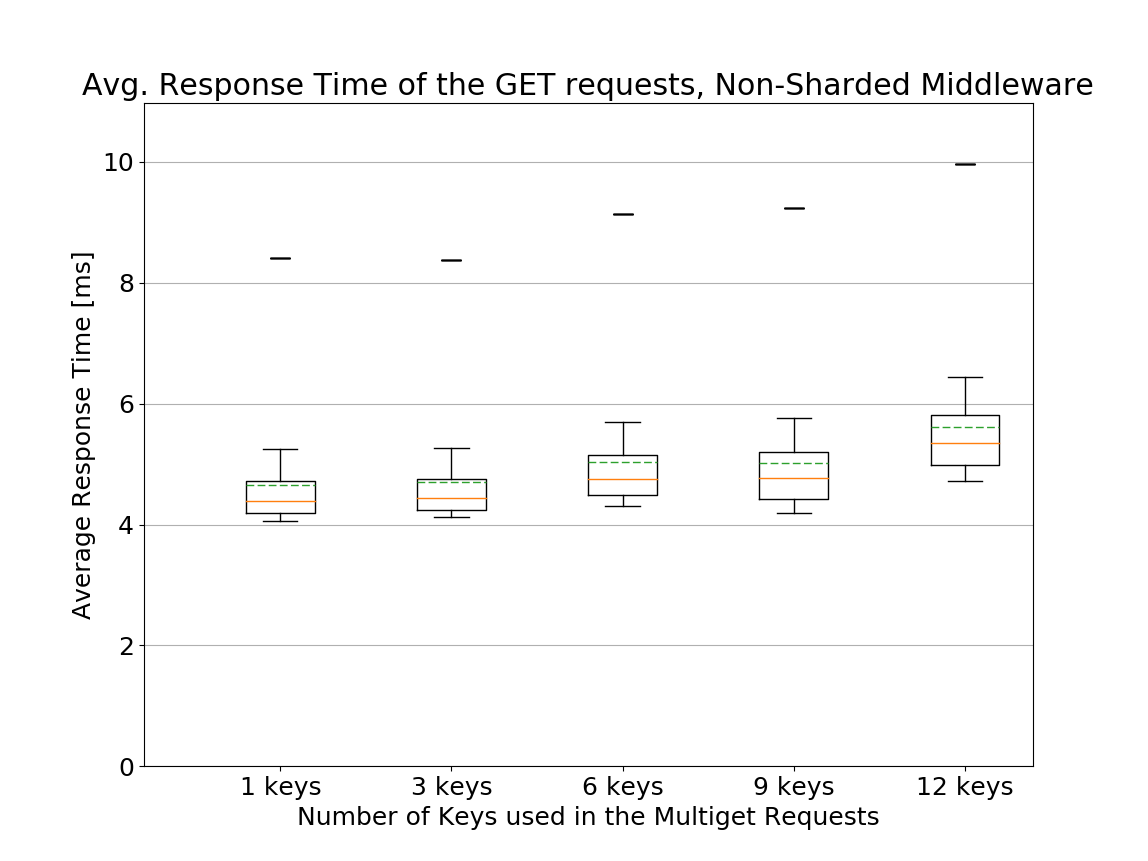
\includegraphics[width=0.5\textwidth]{plots/reads/non_sharded_get_with99.png}
\caption{Response Times of the Non-Sharded Middleware experiment as measured on the clients and evaluated for the GET requests. Legend in Figure \ref{fig:boxplot_legend}.}
\label{plt:non_sharded_get_with99}
\end{figure}


\subsection{Histogram}\label{sub:histogram}
%https://blog.newrelic.com/2017/11/15/expected-distributions-website-response-times/
In the following we will have a look at the histograms of the response times of MULTIGET requests with 6 keys as measured on the client and inside the middleware both, for sharded and non-sharded mode. As the network latencies between different VMs can be different (up to 1ms) the distributions of the response times get shifted by that amount. This means that if we would take the union of the response times and plot the corresponding histogram we would likely get a distribution that does not properly reflect the situation as we could suddenly have two peaks for example. Motivated by that we checked whether the distributions for the individual machines looked similar and then plotted the histograms for one middleware and one client (with one memtier instance) in Figure \ref{plt:hist:single_vms}. In order to make the results better comparable we divided the absolute response time occurrences by the total number of requests (for each machine) which gives us the relative occurrences and a graph which is basically a probability density function. Furthermore we set the upper limit to 10ms because as we have seen this roughly corresponds to the 99-percentile for the clients (which means even higher for the middlewares) and therefore we cover most of the occurrences.\\

As we would have guessed from the box plots in the previous two subsections the response times do not seem to be normal distributed as they show quite a long tail. This corresponds more to a log-normal distribution which is what we often see for the response times of systems such as web services \cite{resp_time_dist}. \\
When comparing the sharded with the non-sharded cases we see that for the former the mode is higher coming from the fact that the response times are distributed more densely around the mode. This results in a median which is roughly 0.5 ms higher in the sharded case which will also be very illustrative in subsection \ref{sub:read:summary} (e.g in Figure \ref{plt:read:mix_get_without99}). This observation could be explained with our misty-2-key effect in subsection \ref{sub:sharded}. There we could observe that a GET request with one key has a significant shorter response time than one with 2 keys. As we saw a MULTIGET payload with 6 keys has on average 5 keys which means two servers get a 2-key request and one a 1-key. These two facts imply that the majority of our response times will be split over a larger interval than in the non-sharded case resulting in a lower and flatter mode in the histogram. Exactly the opposite could be observed when changing the number of keys to 12 for which we plotted the result of the middleware in Figure \ref{plt:hist:single_vms_12_keys}. There we see that the response times in the sharded case are much more predictive. This can be explained with the fact that in sharded mode we expect less variance for the response times since we always have to wait until the slowest server responds. 


\begin{figure}
\centering
\begin{subfigure}{.5\textwidth}
    \centering
    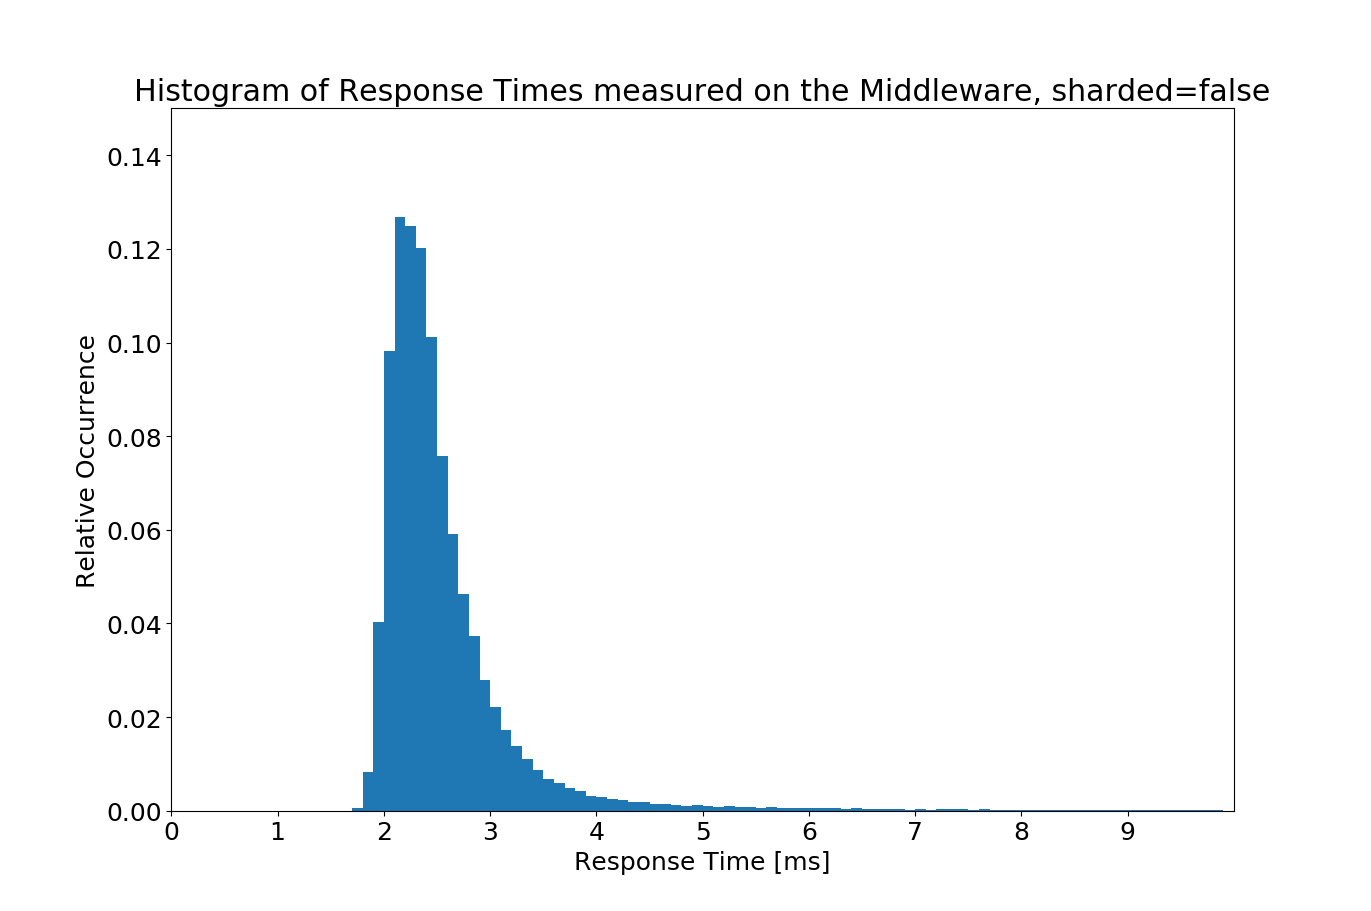
\includegraphics[width=\textwidth ]{plots/reads/histogram/single_vms/mw_non_sharded.png}
    \caption{Middleware Non-Sharded}
    \label{plt:hist:single_mw_non_shard}
\end{subfigure}%
\begin{subfigure}{.5\textwidth}
    \centering
    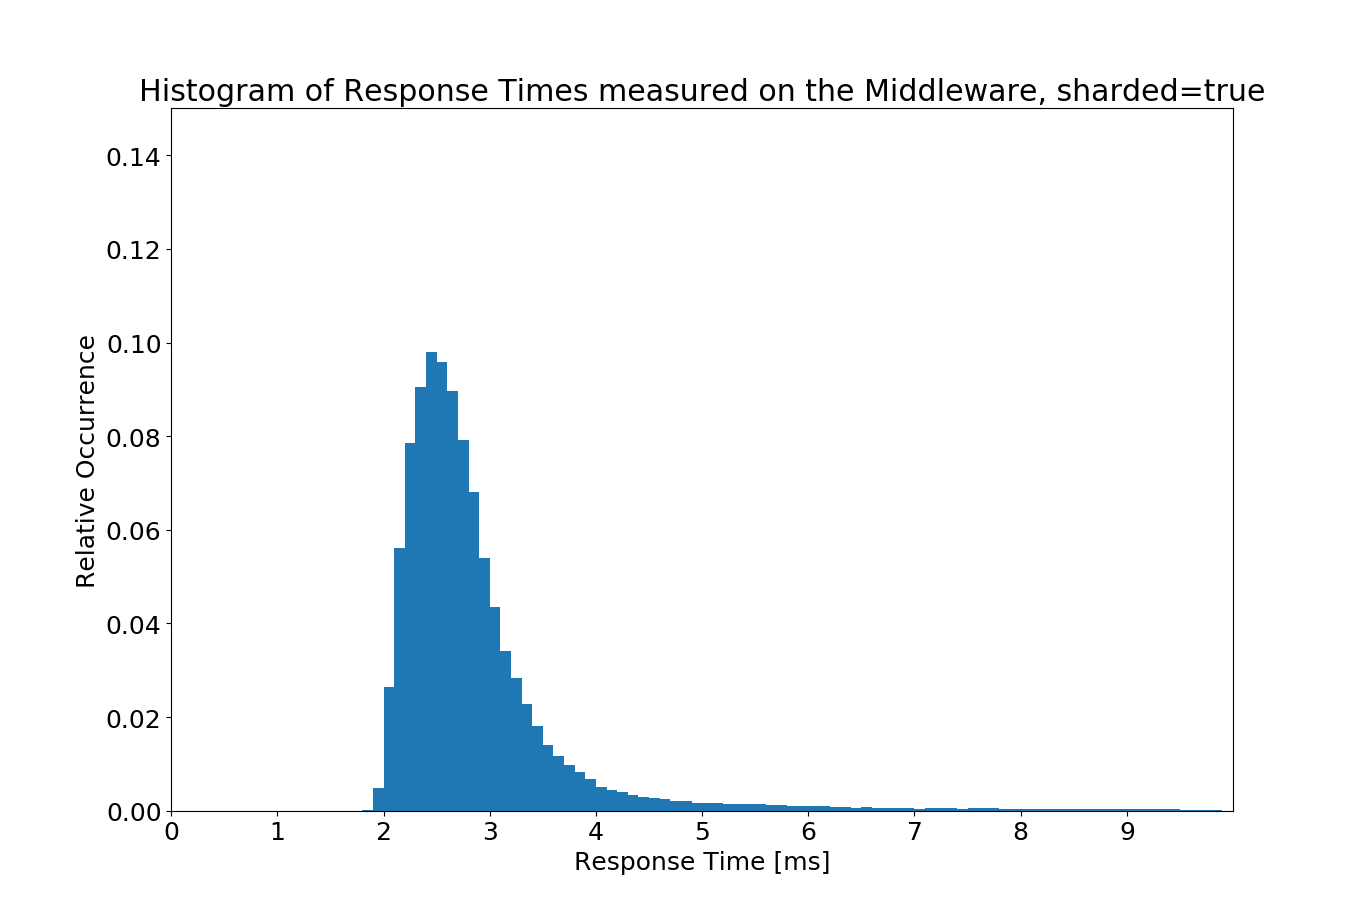
\includegraphics[width=\textwidth ]{plots/reads/histogram/single_vms/mw_sharded.png}
    \caption{Middleware Sharded}
    \label{plt:hist:single_mw_shard}

\end{subfigure}
\begin{subfigure}{.5\textwidth}
    \centering
    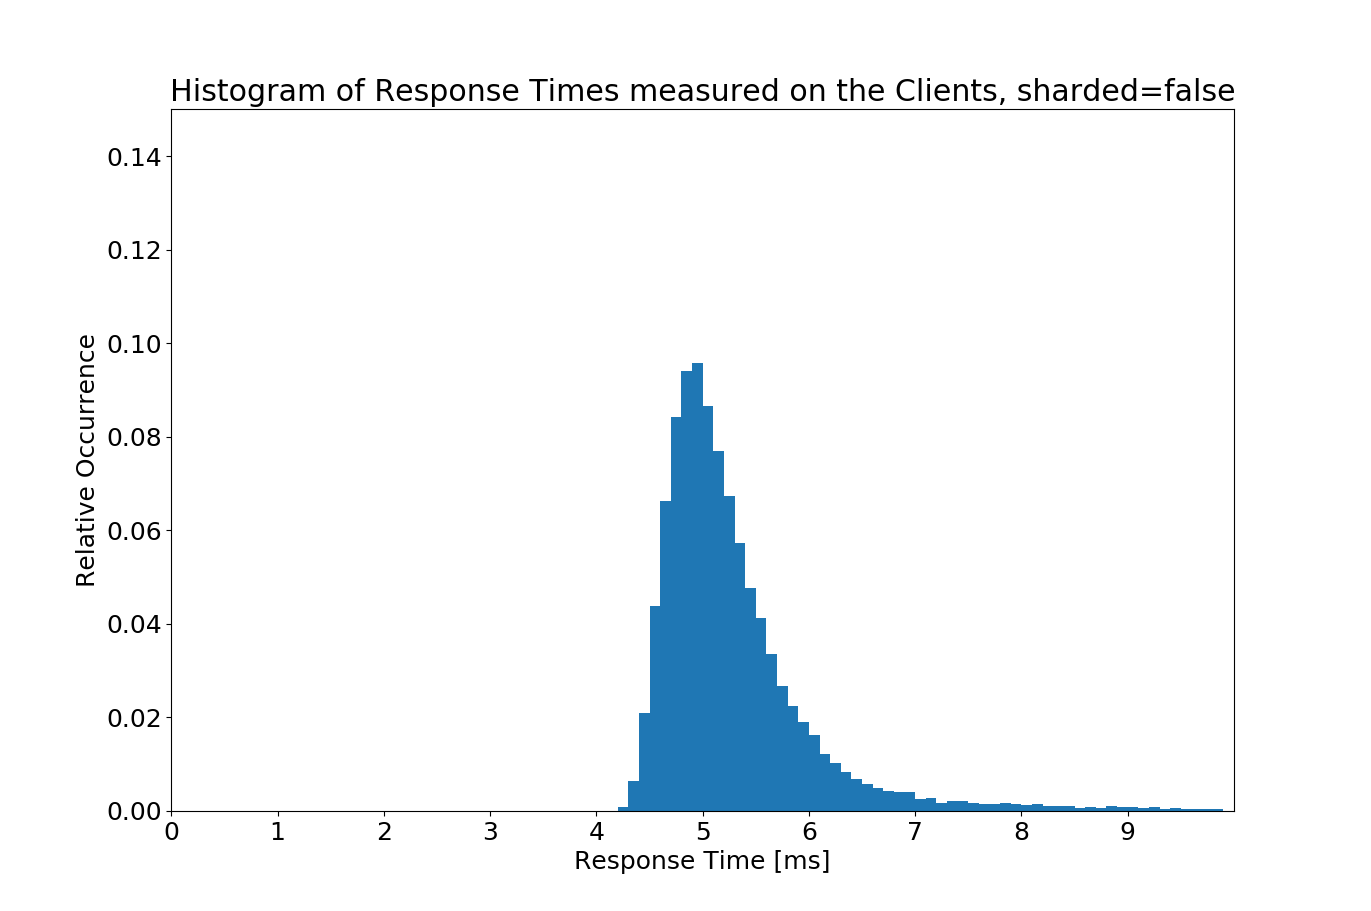
\includegraphics[width=\textwidth ]{plots/reads/histogram/single_vms/client_non_sharded.png}
    \caption{Client Non-Sharded}
    \label{plt:hist:single_client_non_shard}

\end{subfigure}%
\begin{subfigure}{.5\textwidth}
    \centering
    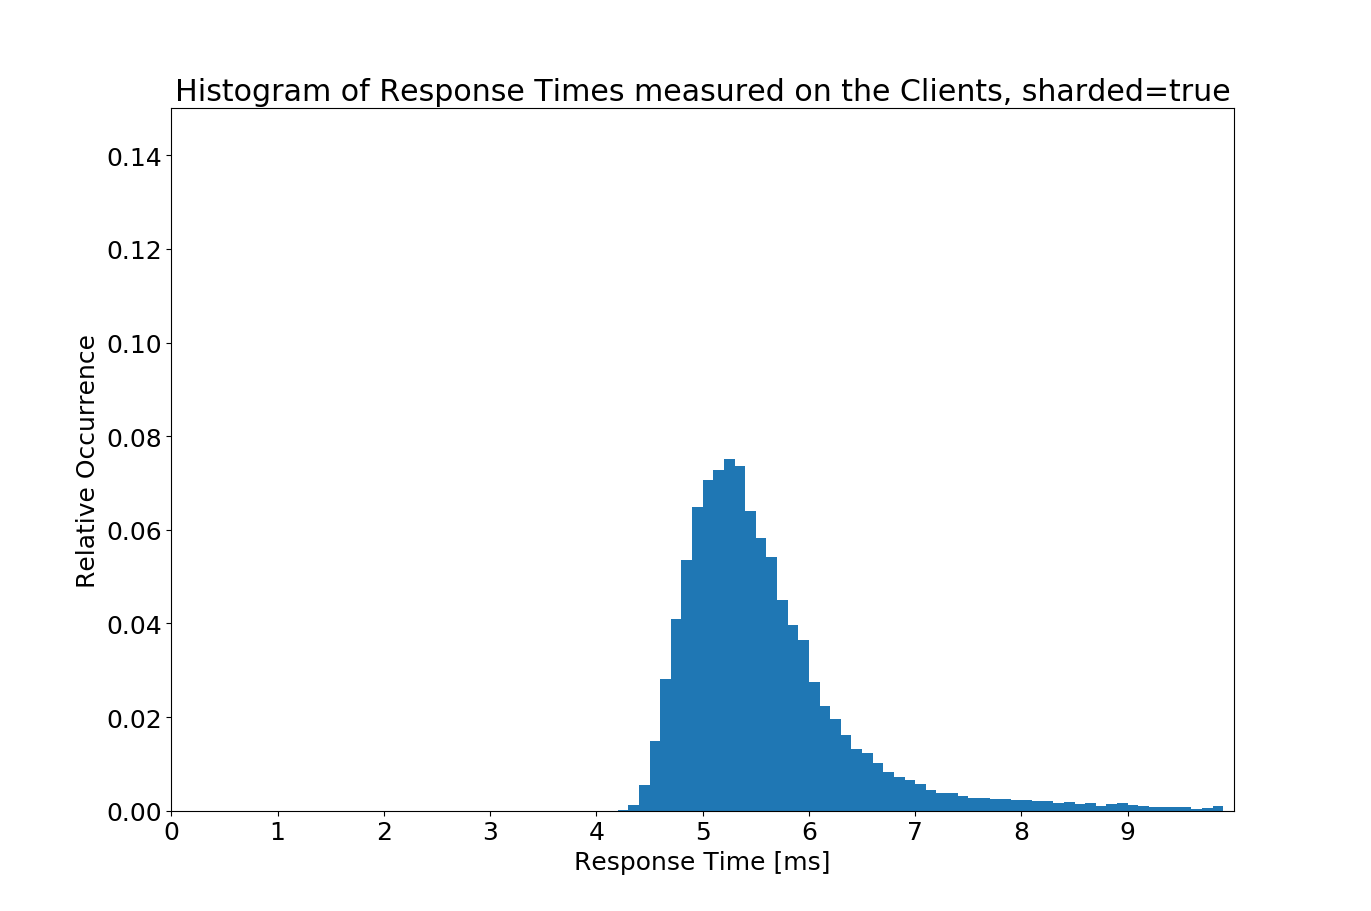
\includegraphics[width=\textwidth ]{plots/reads/histogram/single_vms/client_sharded.png}
    \caption{Client Sharded}
    \label{plt:hist:single_client_shard}

\end{subfigure}
\caption{Density plots for the response times of MULTIGETs with \tb{6 keys} as measured on the middleware and on the client with sharding enabled and disabled.}
\label{plt:hist:single_vms}
\end{figure}


\begin{figure}
\centering
\begin{subfigure}{.5\textwidth}
    \centering
    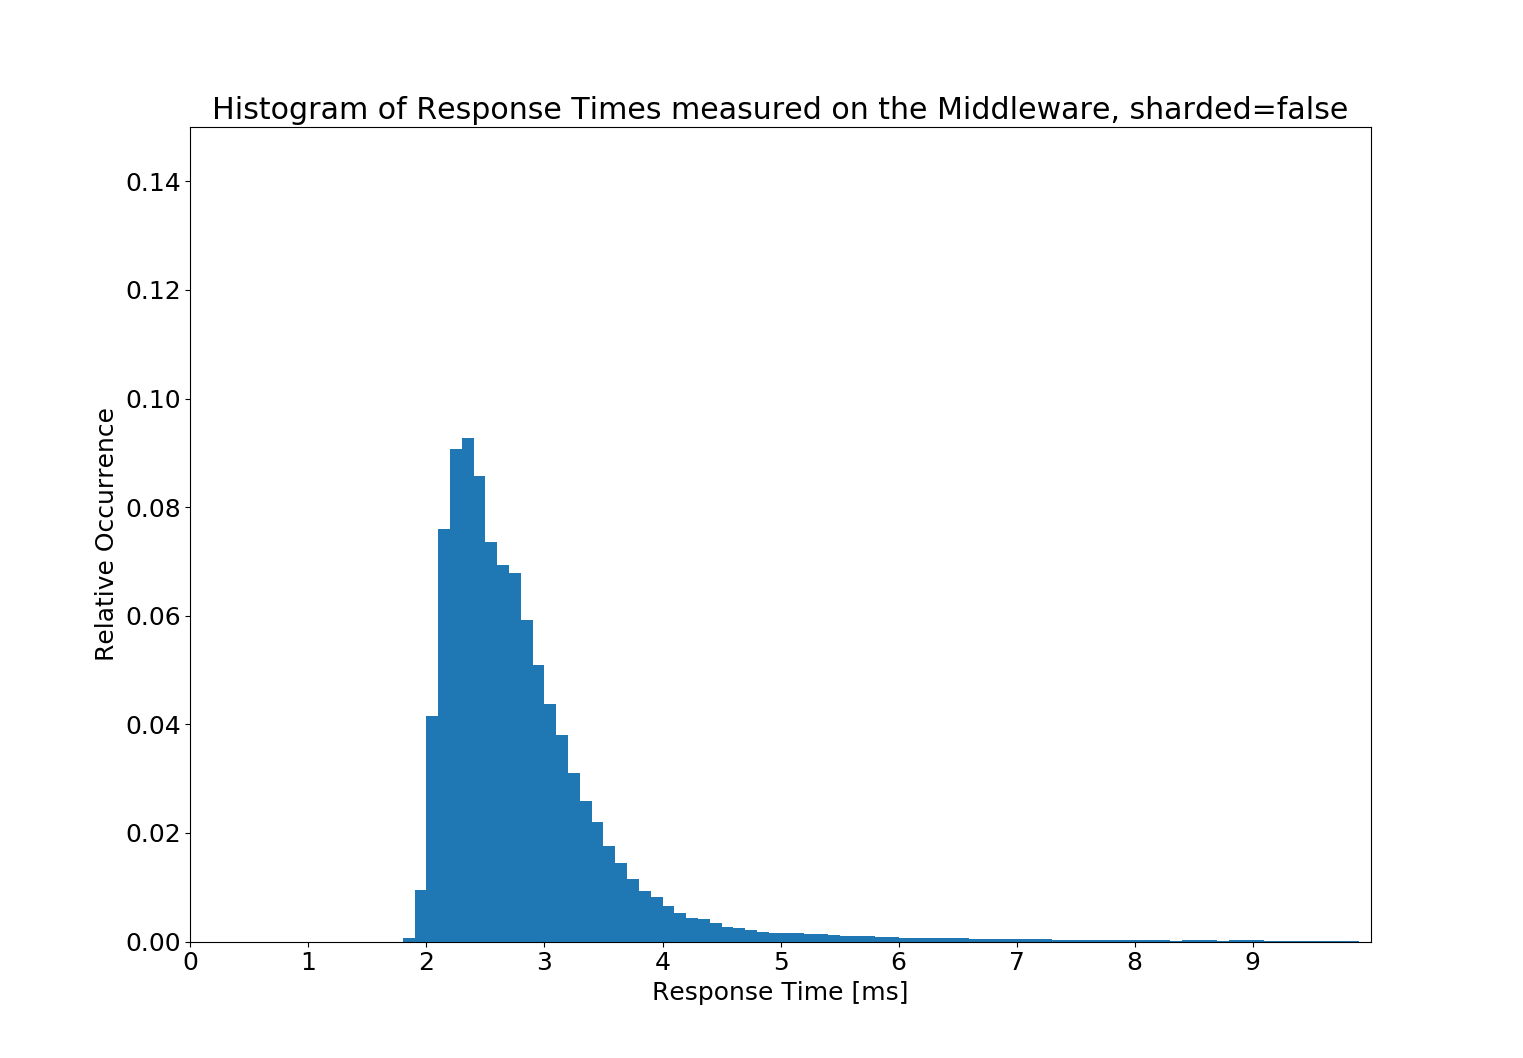
\includegraphics[width=\textwidth ]{plots/reads/histogram/single_vms/mw_non_sharded_12_keys.png}
    \caption{Middleware Non-Sharded}
    \label{plt:hist:single_mw_non_shard_12_keys}
\end{subfigure}%
\begin{subfigure}{.5\textwidth}
    \centering
    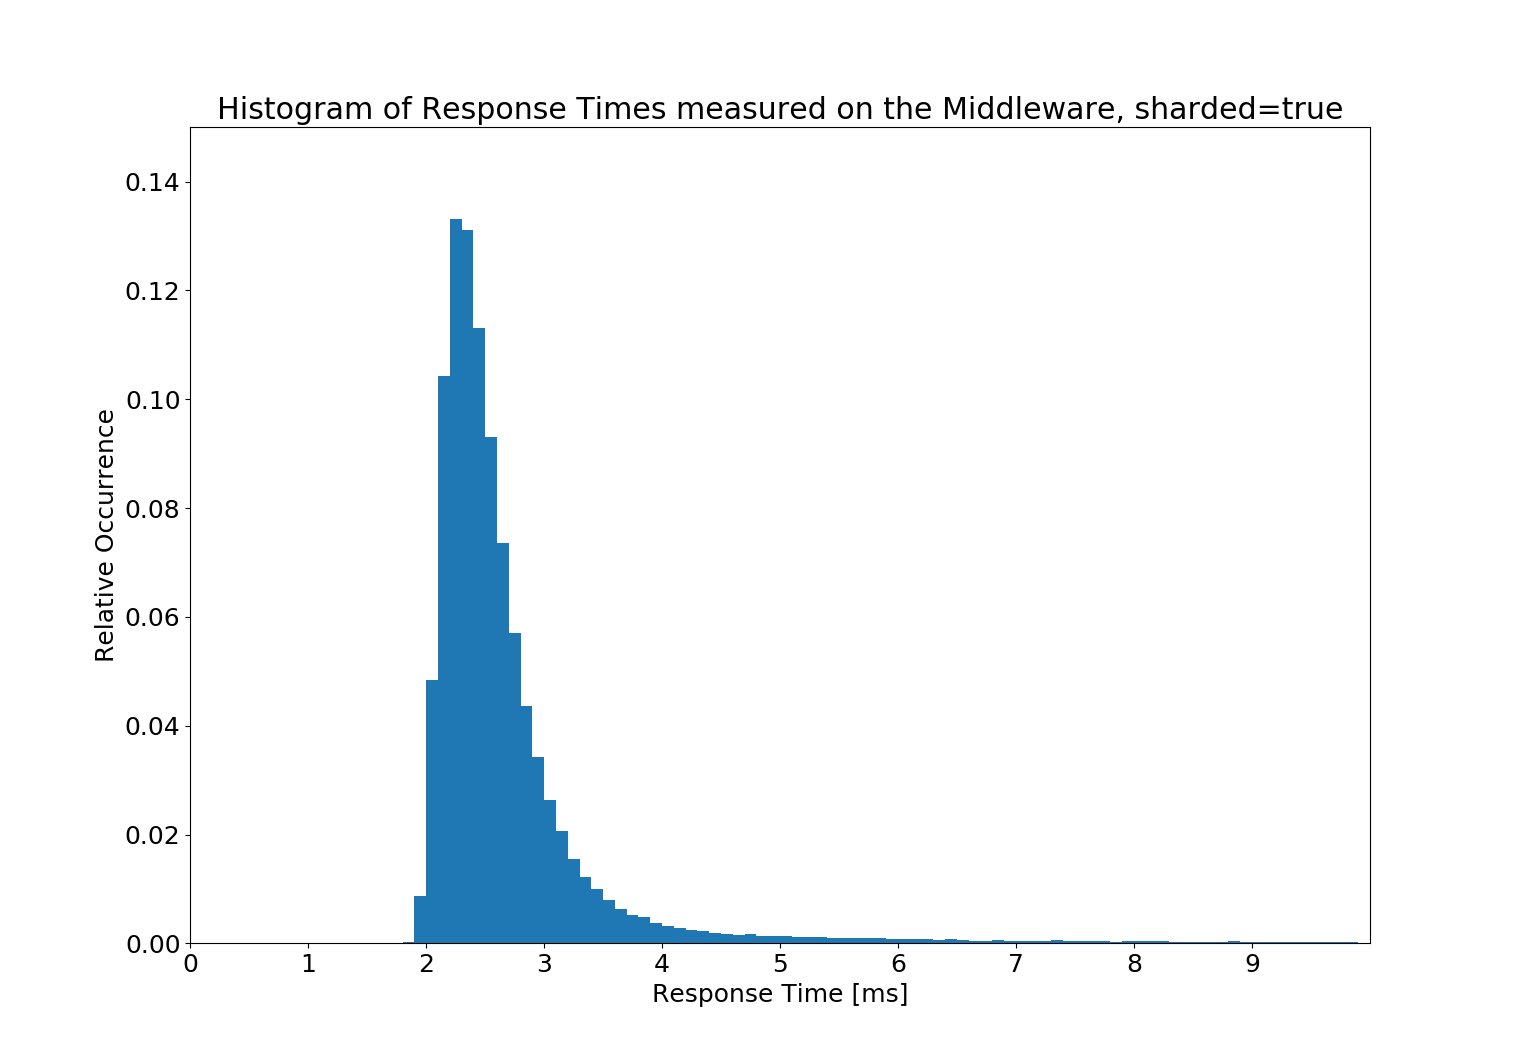
\includegraphics[width=\textwidth ]{plots/reads/histogram/single_vms/mw_sharded_12_keys.png}
    \caption{Middleware Sharded}
    \label{plt:hist:single_mw_shard_12_keys}
\end{subfigure}
\caption{Density plots for the response times of MULTIGETs with \tb{12 keys} as measured on the middleware with sharding enabled and disabled.}
\label{plt:hist:single_vms_12_keys}
\end{figure}



\subsection{Summary}\label{sub:read:summary}
From subsection \ref{sub:sharded} we know that for our set of keys the service times and therefore also the response times for the MULTIGETs increase for 3 keys due to the replication overhead and then remain more or less fixed. In the non-sharded mode we know from subsection \ref{sub:non_sharded} that the service times (and therefore also response time) first stay constant and then increase with increasing number of keys. These two facts together imply that there should be a sweet-spot after which it is worth to use sharding. In order to find this point we make use of Figure \ref{plt:read:mix_get_without99} which merges the two figures \ref{plt:sharded_get_with99} and \ref{plt:non_sharded_get_with99} of the mentioned two subsections and compares them. We left out the 99-percentiles and chose different scale of the y-axis for the favour of better distinguishability. In addition we summarized the service times measured on the middleware for the MULTIGETs both for the sharded and non-sharded case in Table \ref{tbl:read:summary}. The discrepancies between the table and the plot in terms of response time arise firts from the fact of having a mixed (GET, MULTIGET) payload generated by memtier which we can not differentiate at the clients and second from the misty-2key-effect which both were explained in detail in the corresponding subsections. \\
We see that for 1 key there is no difference since our implementations treats requests with a single key independently from the sharding-mode. For three keys we see the overhead of splitting the request to multiple servers in the sharded mode while for the non-sharded case the response time did not change. For 6 keys we have even a larger difference due to the mentioned effect described in subsection \ref{sub:sharded}. Finally, for 9 keys we see that the response time in the sharded case is smaller than in non-sharded mode which means the size of the request brings more overhead than replicating three smaller requests to all servers. This difference even becomes more demonstrative for 12 keys. Due to these observation we claim that from a MULTIGET request size of 9 keys it is worth to use the sharded mode.

\begin{figure}[H]
\centering
    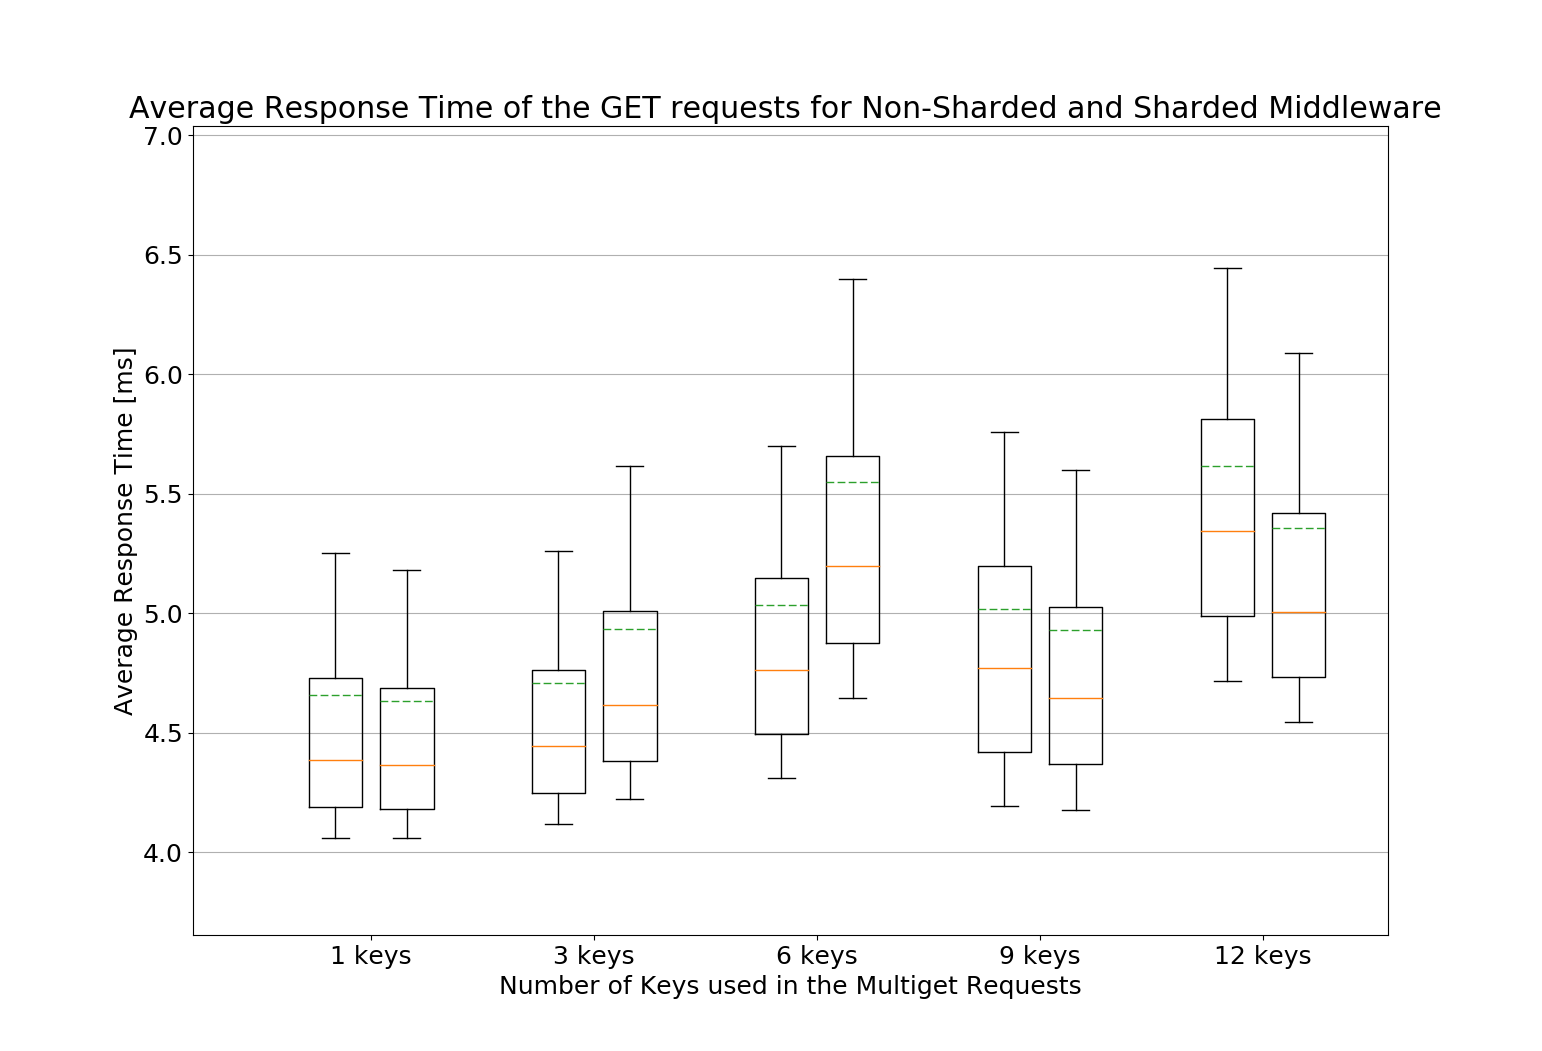
\includegraphics[width=0.6\textwidth]{plots/reads/mixed_get_without99.png}
\caption{Comparison of the results for the GET response times measured on the clients depending on the number of keys and the mode of the middleware. The boxes on the left hand-side correspond to the non-sharded and those on the right to the sharded mode. The legend for the boxes can be found in Figure \ref{fig:boxplot_legend}.}
\label{plt:read:mix_get_without99}
\end{figure}

\begin{table}[H]
\centering
    \scriptsize{
		\begin{tabular}{|l||c|c|c|c|c|} \hline 
		\tb{Keys}                           & \tb{1}    &      \tb{3}     &     \tb{6}       &   \tb{9}  &       \tb{12}   \\ \hhline{|=|=|=|=|=|=|}  
        Sharded MULTIGET Service Time       &   2.3    &        2.6   &      3.0    &     2.6   &      2.7 \\ \hline
        Non-Sharded MULTIGET Service Time   &   2.3    &    2.3     &    2.5       &  2.7        & 2.9      \\ \hline
		\end{tabular}
	}
    \caption{Comparison of the Sharded and Non-Sharded averaged service times in milliseconds as measured for the MULTIGET requests on the two middlewares.}
    \label{tbl:read:summary}
\end{table}


\section{2K Analysis (90 pts)}

In this section we perform a 2k analysis based on a 2k experiment with 3 repetitions for the following parameters and corresponding levels.

\begin{itemize}
	\item Memcached servers: 2 and 3
	\item Middlewares: 1 and 2
	\item Worker threads per MW: 8 and 32
\end{itemize}

Each experiment was be conducted for (a)~a write-only, (b)~a read-only, and (c)~a 50-50-read-write workload each analyzed separately in a corresponding subsection. We will investigate on the impact of the mentioned parameters on the throughput and response time as measured on the clients.  For all experiments we used 3 load generating machines and the number of virtual clients per memtier-thread was chosen to be 32. This gives a total of $3 \times 2 \times 32 = 192$ clients which should be okay to saturate a system with 32 worker threads and two middlewares as we have seen in the baseline experiments. The remaining parameters can be found in the below table.

%Mention saturated system

\begin{center}
	\scriptsize{
		\begin{tabular}{|l|c|}
			\hline Number of servers                & 2 and 3                                     \\ 
			\hline Number of client machines        & 3                                           \\ 
			\hline Instances of memtier per machine & 2                                           \\ 
			\hline Threads per memtier instance     & 1                                           \\
			\hline Virtual clients per thread       & 32                                     \\ 
			\hline Workload                         & Write-only, Read-only, and 50-50-read-write \\
			\hline Multi-Get behavior               & N/A                                         \\
			\hline Multi-Get size                   & N/A                                         \\
			\hline Number of middlewares            & 1 and 2                                     \\
			\hline Worker threads per middleware    & 8 and 32                                    \\
			\hline Repetitions                      & 3                                   \\ 
			\hline Duration                         & 60 seconds        \\
			\hline 
		\end{tabular}
	} 
\end{center}

\subsection{Procedure and References}
For this section we heavily made use of chapter 18 in the following book \cite{performance_book} and therefore also use it's terminology. All data regarding this section can be found in this folder\footnote{\url{https://gitlab.ethz.ch/siegli/asl-fall17-project/tree/master/experiment_outputs/useful/2k_analysis}}. It contains the raw data as well as the spread-sheet which was used to evaluate the result in a sign-table approach. Our model has 8 parameters : Independent (\tb{I}) the bias of our model used to explain the expected mean;  Middlewares (\tb{M}), Workers (\tb{W}) and Servers (\tb{S}) used to explain the effect of our three parameters we are interested in; any combination between these three used to explain interactions among them and finally an \tb{ERROR} which is used to explain any experimental variation. Based on the sign table we first calculated the effects and then based on the sum of squares of the effects and the total sum of squares (not shown in the tables) we derived the percentage of variation used for explaining the impact of the corresponding parameter on throughput respectively response time. For the complete formulas we refer to \cite{performance_book} page 309. From the interactive law we know that the response time is indirect proportional to the throughput ($RT \propto \frac{1}{TP}$) we performed the analysis for the response times based on the inverses of the RT measurements. This also makes sense intuitively since lower response time means "better". For the analysis we will only consider throughput and take the results for the response times as sanity check. By looking at the output files of the middleware we could see that the queue lengths and queue waiting times in any experiment were sufficiently large to consider the system saturated which is important for doing the analysis. We also considered a multiplicative model out of interest but the outcomes were nearly identical to the additive we used. Furthermore, there were no signs (such as high $y_{max}/y_{min}$ ratio) additionally motivating the choice of using the simpler additive model.

\subsection{Write-Only Payload}
Figure \ref{img:2k:wo} tells us that for a write-only payload the average throughput was 19k rps. From the percentage of variation we derive that the throughput is mostly affected by the number of workers (8 vs. 32), followed by the number of middlewares (1 vs. 2). The interactive effects of the parameters and also the error are small. This outcome maps to what we could observe in subsection \ref{sub:heavy_load} where we also compared one vs. two middlewares for different worker scenarios and a write-only payload. There we saw that for 32 workers we gain not that much by using a second middleware compared to what we gain by switching from 8 to 32 which was explained in that subsection. Visually this is nicely illustrated in Figure \ref{plt:bl:one_two_middleware_3cl}. From section \ref{sec:writes} we know that adding more servers is rather disadvantageous for a write-only payload since the servers are not the bottleneck and we increase the overhead of replication. This might explain the low contribution to throughput by the S parameter. 

\begin{figure}[H]
    \centering
    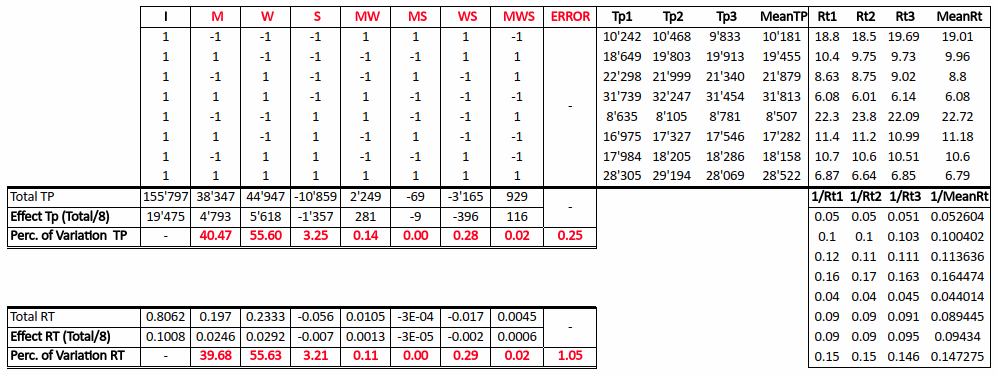
\includegraphics[width=\textwidth]{images/2k_analysis/write-only-table.png}
    \caption{Sign Table for the WRITE-ONLY payload.}
    \label{img:2k:wo}
\end{figure}

\subsection{Read-Only Payload}
Looking at Figure \ref{img:2k:ro} we see that we have a higher average throughput of 25k rps for a read-only payload. Moreover, the contribution to throughput by the number of middlewares and number of workers shrinks down to $\approx 15\%$. The throughput is mostly affected by the number of servers (2 vs. 3). These observations also match with what we could observe in sections \ref{sec:bl_without_mw} and \ref{sec:bl_with_mw} where we saw that the bandwidth limit per server is roughly 11k rps. As the servers now are the bottlenecks it intuitively makes sense that adding one more has a big impact on throughput. The limits of 22k rps and 33k rps can also very nicely be seen in the table of Figure \ref{img:2k:ro} as well as in the \tt{dstat} files of the servers\footnote{\url{https://gitlab.ethz.ch/siegli/asl-fall17-project/blob/master/experiment_outputs/useful/2k_analysis/2k_experiment/dstat_server1.txt}}. In addition to the write-only payload we do not introduce more overhead by adding a third server (as long as the latencies are comparable which they are) because we do not have to replicate the messages. The fact that we do not have the replication overhead also explains the higher average throughput as we can go up to 33k rps. As throughput is bound by the servers it does not really matter whether we increase the number of middlewares or the number of workers since both have their upper limits at the throughput defined by the servers i.e. 22k rps and 33k rps. Finally, it is also this fact which makes the M and W parameters highly correlate resulting in a cross-correlation factor MW which contributes nearly as much to the variations as the original parameters do.

\begin{figure}[H]
    \centering
    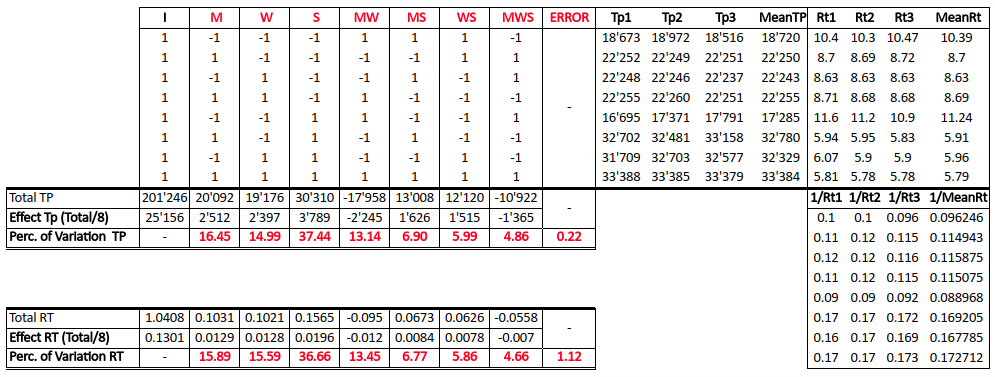
\includegraphics[width=\textwidth]{images/2k_analysis/read-only-table.png}
    \caption{Sign Table for the READ-ONLY payload}
    \label{img:2k:ro}
\end{figure}

\subsection{Mixed Payload}
Last, we have a look at a mixed payload which defaults to a SET:GET request ratio of 1:1 by the memtier clients. We see that the average throughput is nearly identical to the read-only payload but when looking at the numbers of the different experiments we see that we achieve a peak throughput of up to 39k rps which is significantly higher than the previous 33k rps. As for the write-only payload the number of workers seems to affect throughput most, followed by the number of middlewares. By comparing the MeanTP entries in the table with those of the other two payloads we observe that the mixed payload seems to help us in overcoming the bandwidth limits of the server (e.g for 2 MW, 32W, 2S) and also reduces the replication overhead in all cases due to the fact that we additionally have "low-overhead" GET requests. However, adding one more server and therefore having a higher bandwidth limit does not pay off the overhead introduced by the additional replication. This can be seen by comparing the lower four with the upper four rows in the Sign Table of Figure \ref{img:2k:mixed} (14k vs. 13k, 24k vs. 23k, 26k vs. 23k and 39 vs. 37k requests per second). The theory can also be verified by looking at the middleware output files for 2 and 3 servers where we see that the service time and therefore also the response times increase for 3 servers. As the increasing number of servers is counterproductive for the throughput, our S parameter is not significantly contributing to the variance and it is the number of middlewares and workers which explain most of the throughputs variance like in the write-only payload scenario.

Likewise in the other two payloads we also have very low contribution to the variation due to experimental errors. This is good since it gives us more confidence for the results of the other parameters.

\begin{figure}[H]
    \centering
    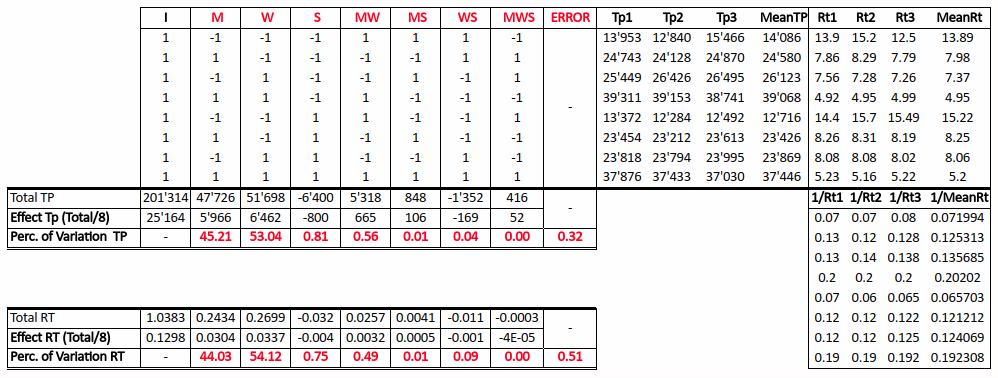
\includegraphics[width=\textwidth]{images/2k_analysis/mixed-table.png}
    \caption{Sign Table for the MIXED (1:1) payload}
    \label{img:2k:mixed}
\end{figure}


\subsection{Summary}
We have seen that the payload type has a huge impact on the measured throughput as each scratches at different boundaries of our system. While for the write only-payload the throughput is upper bound by the overhead introduced with replication it is the servers bandwidth which hinders us from going over 33k rps in a read-only payload. The mixed payload brings a compromise which allows us to go up to the servers bandwidth with the (less overhead) GET requests and still having the same amount of SET requests to go even further. Therefore, we claim that it is only a mixed payload which can achieve the peak performance of our system including all the machines. Note that this does not imply that it is better than the other two payloads for any configuration. A counterexample would be: 1 middleware, 32 workers, 1 server (second to last row in Sign Tables) for which we achieve 32k rps in a read-only payload and only 23 in a mixed payload because the replication overhead seems to be too big. 

\section{Queuing Model (90 pts)}

In this section we want to model our system using different types of Queueing Models and see how good they can predict our measurements.

\subsection{M/M/1}
In a first step we will model our entire system as one "black-box" M/M/1 queue. For each worker configuration we will derive a separate model and choose the parameters at the maximal throughput points which are listed in the table of subsection \ref{sub:writes:summary}. An M/M/1 is completely defined by the arrival rate $\lambda$ and service rate $\mu$. We will use the queue of the model to model the queue between the networking thread and the workers. The worker threads in our system will be modeled as one service. The input to our model will be the throughput and the service time ("average time waiting for memcached" in the table and refered to as measured\_service\_time from now on) as measured on the middleware. From these we derive $\lambda$ and $\mu$ which allows us to predict the remaining values. For $\lambda$ we will take half of the measured throughput because as we are in a closed network the output rate equals the input rate and because we measured throughput for two middlewares (throughput is summed up) we divide by two. This should be fine since our goal is to only predict average values anyhow. For the service time $\mu$ we will chose $\frac{\#workers}{measured\_service\_ time}$ since we want to express that we are faster with a higher number of workers. For the calculation of avg. QWT, avg QL and avg. RT we refer to \cite{performance_book} page 525, points 17, 9 and 12 respectively. For calculating avg. QL Little we apply Little's Law to our defined arrival rate and the measured avg. QWT, i.e. avg. QL Little = $\lambda \times$avg. QWT measured.

\begin{table}[H]
    \centering
    \begin{tabular}{|c|c|c|c|c|p{1.5cm}|p{1.5cm}|p{1.5cm}|p{1.5cm}|} \hline
            Workers &      & $\lambda$ & $\mu$   & $\rho = \frac{\lambda}{\mu}$ & avg. QWT   & avg. QL   &  avg. QL Little & avg. RT (MWT)  \\ \Xhline{4\arrayrulewidth}
         \multirow{2}{*}{8} & Measured &     -    &     -        &   -                       &  1.28    &  3.20      &  -                & 3.47 \\ \cline{2-9}
            & Model    &  3621    &      3704   &  0.98                      & 11.75      & 42.54     & 4.63              & 12.02 \\ \Xhline{3\arrayrulewidth}
         
         \multirow{ 2}{*}{16} & Measured &   -      &     -       &   -                   &    1.31       &    7.01           &      -             &    3.59    \\ \cline{2-9}
         & Model    &   6963      &   7143         &       0.97               &    5.40       &       37.63        &      9.12           &   5.54    \\ \Xhline{3\arrayrulewidth}
         
         \multirow{ 2}{*}{32} &Measured &   -      &     -       &   -                   &    2.23       &      14.69         &      -             &   5.73    \\ \cline{2-9}
         & Model    &   8988     &   9249        &      0.97                &      3.72    &      33.46   &        20.04          &  3.83     \\ \Xhline{3\arrayrulewidth}
         
         \multirow{ 2}{*}{64} &Measured &   -      &     -       &   -                   &     3.47      &     33.86          &      -             &    8.73   \\ \cline{2-9}
         & Model    &   11913      &    12284        &      0.97                &    2.61       &      31.13         &     41.34              &    2.69   \\ \hline
    \end{tabular}
    \caption{Result for the M/M/1 model. All time values are given in milliseconds.}
    \label{tab:queueing:mm1}
\end{table}

As we can see from the Table \ref{tab:queueing:mm1}, our model predicts very badly. The main reason might be because an M/M/1 model is not appropriate to model our design of one queue and multiple servers as one M/M/1 queue. In order to come up with an appropriate service rate for only one server we have to choose it's service time very small. We can see that in our model the predicted service time (= avgRT - avg. QWT or 1/$\mu$) leads to the fact that we can not model the correct QWT and RT at the same time.


\subsection{M/M/m}
Next we will investigate an M/M/m model. This has the advantage that we can model the fact that we have multiple worker threads and therefore set the service rate as $\mu = \frac{1}{measured\_service\_time}$. Therefore, the m servers in the model correspond to our m worker threads and the M/M/m queue to the queue between workers and networking thread. The arrival rate was chosen as before. For the formulas used for calculating the values in the table we again link to \cite{performance_book} page 528. 
\begin{table}[H]
    \centering
    \begin{tabular}{|c|c|c|c|c|p{1.2cm}|p{1.4cm}|p{1.4cm}|p{1.4cm}|} \hline
          Workers (m) &         & $\lambda$ & $\mu$   & $\rho = \frac{\lambda}{\mu \times m}$ & avg. QWT   & avg. QL   &  avg. QL Little & avg. RT (MWT)  \\ \Xhline{4\arrayrulewidth}
      \multirow{2}{*}{8} &   Measured &     -    &     -        &   -                       &  1.28    &  3.20      &  -                & 3.47 \\\cline{2-9}
      &   Model    &  3621    &   462 &       0.98  & 11.09   & 40.0  &  4.63    & 13.25 \\ \Xhline{3\arrayrulewidth}
         
     \multirow{2}{*}{16} &    Measured &   -      &     -       &   -                   &    1.31       &    7.01           &      -             &    3.59    \\ \cline{2-9}
       &  Model    &   6963     & 446   &  0.97   & 4.89  & 34.0   &  9.12   &   7.13  \\ \Xhline{3\arrayrulewidth}
         
      \multirow{2}{*}{32} &   Measured &   -      &     -       &   -                   &    2.23       &      14.69         &      -             &   5.73    \\ \cline{2-9}
      &   Model    &   8988    &  289  &   0.97  & 3.13  &  28.0   & 20.04  &   6.59   \\ \Xhline{3\arrayrulewidth}
         
      \multirow{2}{*}{64} &   Measured &   -      &     -       &   -                   &     3.47      &     33.86          &      -             &    8.73   \\ \cline{2-9}
     &    Model    &   11913    & 191   &  0.97   &  1.98 & 24.0  &  41.34     &    7.19  \\ \hline
    \end{tabular}
    \caption{Result for the M/M/m model. All time values are given in milliseconds.}
    \label{tab:queuein:mmm}
\end{table}

Compared to the M/M/1 model we can now see that the real service time (which is in the orders of milliseconds) can be correctly reflected by our model i.e $avg.RT - avg.QWT = measured\_service\_time$. This leads to a pretty good result for the case of 32 and 64 workers. However, our model still struggles in either predicting avg. RT or the avg. QWT precise enough implying the observed discrepancies in avg. QL. 


\subsection{Network of Queues}

Based on section \ref{sec:bl_with_mw} we built a network of queues which simulates our system. Figure \ref{fig:queueing_models} shows the models we will use for analyzing the experiment with one respectively two middlewares. All components will be modeled as M/M/1 queues. For the input parameters we will use the measurements from Table \ref{tbl:baseline_with_mw:measurements}. Arrival rates will be determined by the measured throughput while the service rates will be chosen in the following way. Middleware: $\mu = 1/(avg.\ time\ in\ queue)$, Server: $\mu = 1/(response\ time\ on\ MW - avg.\ time\ in\ queue)$, Clients: $\mu = 1/(response\ time\ on\ client - response\ time\ on\ MW)$. We use the clients in order to simulate the delay introduced by the network. As all the measurements were taken with 54 clients and more we will use this number.  

\begin{figure}
\centering
\begin{subfigure}{.5\textwidth}
    \centering
    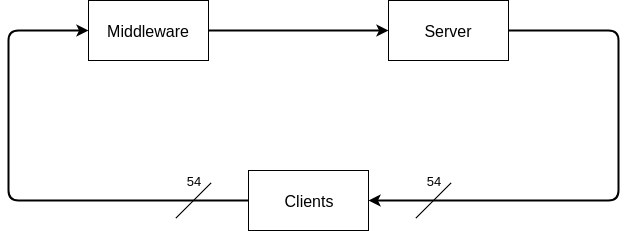
\includegraphics[width=\textwidth ]{images/queueing.png}
    \caption{Single Middleware Model}
    \label{plt:queueing_single_mw}
\end{subfigure}%
\begin{subfigure}{.5\textwidth}
    \centering
    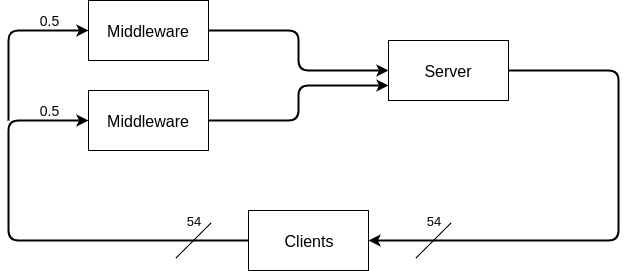
\includegraphics[width=\textwidth ]{images/queueing2.png}
    \caption{Double Middleware Model}
    \label{plt:queuing_two_mw}
\end{subfigure}
\caption{The two models we will use for our network of queues. All components are modelled as M/M/1 queues. The Middleware includes the networking thread as well as the workers and the Server models the memcached server.}
\label{fig:queueing_models}
\end{figure}

The result of the bottleneck analysis is shown in Figure \ref{fig:queueing_bottleneck}. We split the analysis into four cases. Read/Write and One/Two Middlewares. For each we chose a corresponding model as described before. Choosing the service time of the middleware as the QWT has the advantage that the resulting utilization reflects the number of jobs in the middeware queue very precisely due to Little's Law since $utilization = nof.\ req.\ in\ queue = \lambda \times queue\ waiting\ time$. This can be verified by looking at the corresponding summary files\footnote{\url{https://gitlab.ethz.ch/siegli/asl-fall17-project/blob/master/experiment_outputs/useful/baseline_with_mw/baseline_one_mw_extended_3cl/one-mw-extended-3cl-summary-data.txt}}\footnote{\url{https://gitlab.ethz.ch/siegli/asl-fall17-project/tree/master/experiment_outputs/useful/baseline_with_mw/baseline_one_mw}}\footnote{\url{https://gitlab.ethz.ch/siegli/asl-fall17-project/blob/master/experiment_outputs/useful/baseline_with_mw/baseline_two_mw_extended_3clients/two-mw-extended-3cl-summary-plot-data.txt}} (for 64 workers and 54 resp. 240 clients). We see that for one middleware in the read-only case the server seems to be the bottleneck while for the write-only payload the middleware is the limiting factor. This intuitively makes sense since as we saw it is the server which hinders performance from going over 11k rps due to bandwidth restrictions. This effect is even increased when using two middlewares which also makes sense since the load on the server increases while we can distribute it on the middlewares. Using two middlewares in the write-only payload shifts the bottleneck from the middleware to the servers because for the middlewares we split the load and on the server we increase it. The network does not seem to be a limiting factor since having enough clients hides the network latency (we also could have modelled it as zero latency delay center).

\begin{figure}[H]
    \centering
    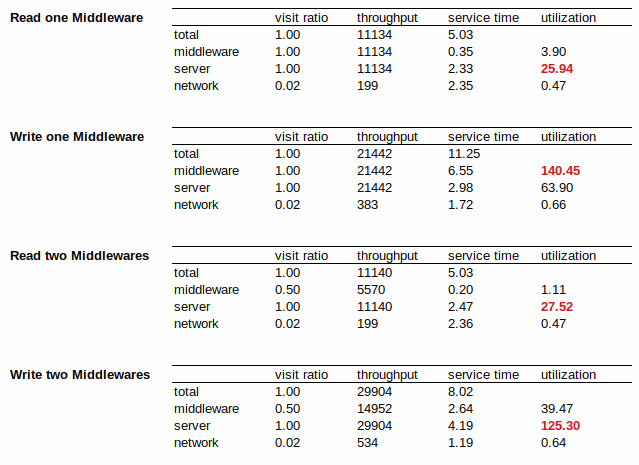
\includegraphics[width=0.7\textwidth]{images/queueing_table.png}
    \caption{Result of the bottleneck analysis done for the experiments in section \ref{sec:bl_with_mw} using the model \ref{plt:queueing_single_mw} for a single middleware and \ref{plt:queuing_two_mw} for two middlewares. \ref{sec:bl_with_mw}}
    \label{fig:queueing_bottleneck}
\end{figure}


\newpage

% Bibliography
\begin{thebibliography}{40}

\bibitem{memcached_protocol}
"Memcached Protocol"\\
\url{https://github.com/memcached/memcached/blob/master/doc/protocol.txt}\\

\bibitem{wireshark}
"Wireshark Packet Inspector"\\
\url{https://www.wireshark.org/} \\

\bibitem{resp_time_dist}
"What Is the Expected Distribution of Website Response Times?"\\
\url{https://blog.newrelic.com/2017/11/15/expected-distributions-website-response-times/}\\

\bibitem{performance_book}
"The Art of Computer Systems Performance Analysis: Techniques for Experimental Design, Measurement, Simulation, and Modeling", Raj Jain,
ISBN: 978-0-471-50336-1\\
\url{http://eu.wiley.com/WileyCDA/WileyTitle/productCd-0471503363.html}\\

\end{thebibliography}

\end{document}




